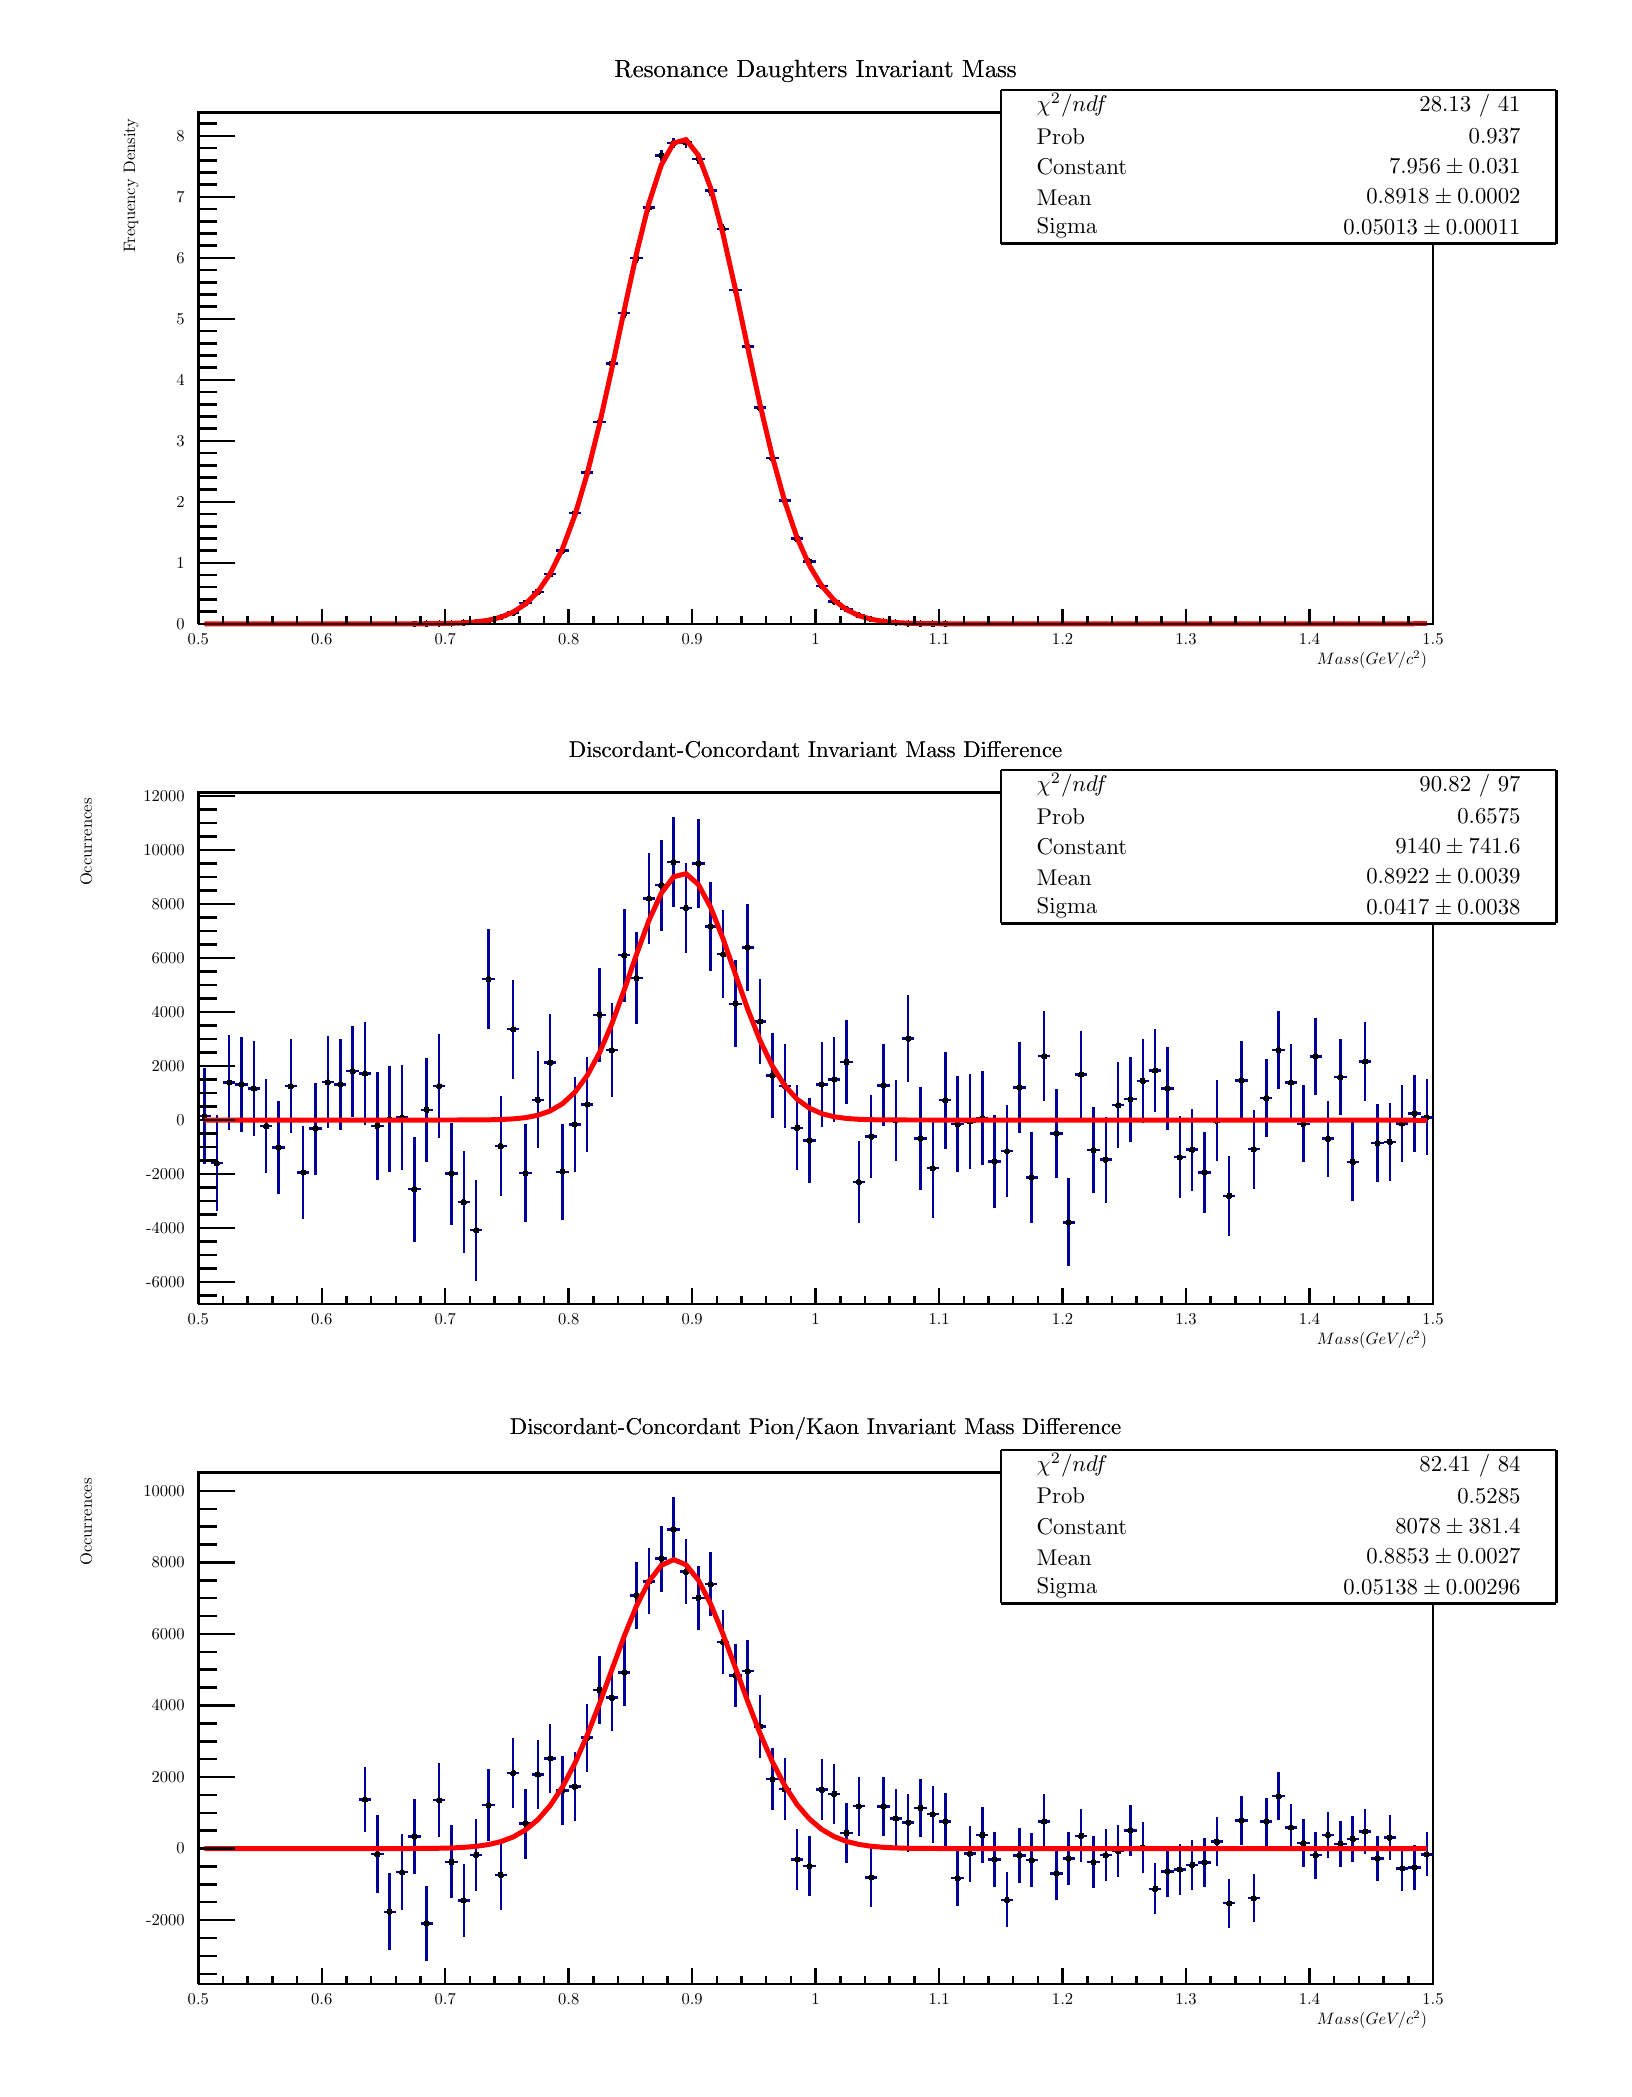
\begin{tikzpicture}
\pgfdeclareplotmark{cross} {
\pgfpathmoveto{\pgfpoint{-0.3\pgfplotmarksize}{\pgfplotmarksize}}
\pgfpathlineto{\pgfpoint{+0.3\pgfplotmarksize}{\pgfplotmarksize}}
\pgfpathlineto{\pgfpoint{+0.3\pgfplotmarksize}{0.3\pgfplotmarksize}}
\pgfpathlineto{\pgfpoint{+1\pgfplotmarksize}{0.3\pgfplotmarksize}}
\pgfpathlineto{\pgfpoint{+1\pgfplotmarksize}{-0.3\pgfplotmarksize}}
\pgfpathlineto{\pgfpoint{+0.3\pgfplotmarksize}{-0.3\pgfplotmarksize}}
\pgfpathlineto{\pgfpoint{+0.3\pgfplotmarksize}{-1.\pgfplotmarksize}}
\pgfpathlineto{\pgfpoint{-0.3\pgfplotmarksize}{-1.\pgfplotmarksize}}
\pgfpathlineto{\pgfpoint{-0.3\pgfplotmarksize}{-0.3\pgfplotmarksize}}
\pgfpathlineto{\pgfpoint{-1.\pgfplotmarksize}{-0.3\pgfplotmarksize}}
\pgfpathlineto{\pgfpoint{-1.\pgfplotmarksize}{0.3\pgfplotmarksize}}
\pgfpathlineto{\pgfpoint{-0.3\pgfplotmarksize}{0.3\pgfplotmarksize}}
\pgfpathclose
\pgfusepathqstroke
}
\pgfdeclareplotmark{cross*} {
\pgfpathmoveto{\pgfpoint{-0.3\pgfplotmarksize}{\pgfplotmarksize}}
\pgfpathlineto{\pgfpoint{+0.3\pgfplotmarksize}{\pgfplotmarksize}}
\pgfpathlineto{\pgfpoint{+0.3\pgfplotmarksize}{0.3\pgfplotmarksize}}
\pgfpathlineto{\pgfpoint{+1\pgfplotmarksize}{0.3\pgfplotmarksize}}
\pgfpathlineto{\pgfpoint{+1\pgfplotmarksize}{-0.3\pgfplotmarksize}}
\pgfpathlineto{\pgfpoint{+0.3\pgfplotmarksize}{-0.3\pgfplotmarksize}}
\pgfpathlineto{\pgfpoint{+0.3\pgfplotmarksize}{-1.\pgfplotmarksize}}
\pgfpathlineto{\pgfpoint{-0.3\pgfplotmarksize}{-1.\pgfplotmarksize}}
\pgfpathlineto{\pgfpoint{-0.3\pgfplotmarksize}{-0.3\pgfplotmarksize}}
\pgfpathlineto{\pgfpoint{-1.\pgfplotmarksize}{-0.3\pgfplotmarksize}}
\pgfpathlineto{\pgfpoint{-1.\pgfplotmarksize}{0.3\pgfplotmarksize}}
\pgfpathlineto{\pgfpoint{-0.3\pgfplotmarksize}{0.3\pgfplotmarksize}}
\pgfpathclose
\pgfusepathqfillstroke
}
\pgfdeclareplotmark{newstar} {
\pgfpathmoveto{\pgfqpoint{0pt}{\pgfplotmarksize}}
\pgfpathlineto{\pgfqpointpolar{44}{0.5\pgfplotmarksize}}
\pgfpathlineto{\pgfqpointpolar{18}{\pgfplotmarksize}}
\pgfpathlineto{\pgfqpointpolar{-20}{0.5\pgfplotmarksize}}
\pgfpathlineto{\pgfqpointpolar{-54}{\pgfplotmarksize}}
\pgfpathlineto{\pgfqpointpolar{-90}{0.5\pgfplotmarksize}}
\pgfpathlineto{\pgfqpointpolar{234}{\pgfplotmarksize}}
\pgfpathlineto{\pgfqpointpolar{198}{0.5\pgfplotmarksize}}
\pgfpathlineto{\pgfqpointpolar{162}{\pgfplotmarksize}}
\pgfpathlineto{\pgfqpointpolar{134}{0.5\pgfplotmarksize}}
\pgfpathclose
\pgfusepathqstroke
}
\pgfdeclareplotmark{newstar*} {
\pgfpathmoveto{\pgfqpoint{0pt}{\pgfplotmarksize}}
\pgfpathlineto{\pgfqpointpolar{44}{0.5\pgfplotmarksize}}
\pgfpathlineto{\pgfqpointpolar{18}{\pgfplotmarksize}}
\pgfpathlineto{\pgfqpointpolar{-20}{0.5\pgfplotmarksize}}
\pgfpathlineto{\pgfqpointpolar{-54}{\pgfplotmarksize}}
\pgfpathlineto{\pgfqpointpolar{-90}{0.5\pgfplotmarksize}}
\pgfpathlineto{\pgfqpointpolar{234}{\pgfplotmarksize}}
\pgfpathlineto{\pgfqpointpolar{198}{0.5\pgfplotmarksize}}
\pgfpathlineto{\pgfqpointpolar{162}{\pgfplotmarksize}}
\pgfpathlineto{\pgfqpointpolar{134}{0.5\pgfplotmarksize}}
\pgfpathclose
\pgfusepathqfillstroke
}
\definecolor{c}{rgb}{1,1,1};
\draw [color=c, fill=c] (0,0) rectangle (20,25.906);
\draw [color=c, fill=c] (0.2,17.5298) rectangle (19.8,25.647);
\draw [color=c, fill=c] (2.16,18.3415) rectangle (17.84,24.8353);
\definecolor{c}{rgb}{0,0,0};
\draw [c,line width=0.9] (2.16,18.3415) -- (2.16,24.8353) -- (17.84,24.8353) -- (17.84,18.3415) -- (2.16,18.3415);
\definecolor{c}{rgb}{0,0,0.6};
\draw [c,line width=0.9] (4.904,18.3415) -- (4.904,18.3422);
\draw [c,line width=0.9] (4.904,18.3422) -- (4.904,18.343);
\draw [c,line width=0.9] (4.8256,18.3422) -- (4.904,18.3422);
\draw [c,line width=0.9] (4.904,18.3422) -- (4.9824,18.3422);
\definecolor{c}{rgb}{0,0,0};
\foreach \P in {(4.904,18.3422)}{\draw[mark options={color=c,fill=c},mark size=2.402402pt, line width=0.000000pt, mark=*,mark size=1pt] plot coordinates {\P};}
\definecolor{c}{rgb}{0,0,0.6};
\draw [c,line width=0.9] (5.0608,18.3419) -- (5.0608,18.343);
\draw [c,line width=0.9] (5.0608,18.343) -- (5.0608,18.3441);
\draw [c,line width=0.9] (4.9824,18.343) -- (5.0608,18.343);
\draw [c,line width=0.9] (5.0608,18.343) -- (5.1392,18.343);
\definecolor{c}{rgb}{0,0,0};
\foreach \P in {(5.0608,18.343)}{\draw[mark options={color=c,fill=c},mark size=2.402402pt, line width=0.000000pt, mark=*,mark size=1pt] plot coordinates {\P};}
\definecolor{c}{rgb}{0,0,0.6};
\draw [c,line width=0.9] (5.2176,18.343) -- (5.2176,18.3446);
\draw [c,line width=0.9] (5.2176,18.3446) -- (5.2176,18.3461);
\draw [c,line width=0.9] (5.1392,18.3446) -- (5.2176,18.3446);
\draw [c,line width=0.9] (5.2176,18.3446) -- (5.296,18.3446);
\definecolor{c}{rgb}{0,0,0};
\foreach \P in {(5.2176,18.3446)}{\draw[mark options={color=c,fill=c},mark size=2.402402pt, line width=0.000000pt, mark=*,mark size=1pt] plot coordinates {\P};}
\definecolor{c}{rgb}{0,0,0.6};
\draw [c,line width=0.9] (5.3744,18.3455) -- (5.3744,18.3476);
\draw [c,line width=0.9] (5.3744,18.3476) -- (5.3744,18.3498);
\draw [c,line width=0.9] (5.296,18.3476) -- (5.3744,18.3476);
\draw [c,line width=0.9] (5.3744,18.3476) -- (5.4528,18.3476);
\definecolor{c}{rgb}{0,0,0};
\foreach \P in {(5.3744,18.3476)}{\draw[mark options={color=c,fill=c},mark size=2.402402pt, line width=0.000000pt, mark=*,mark size=1pt] plot coordinates {\P};}
\definecolor{c}{rgb}{0,0,0.6};
\draw [c,line width=0.9] (5.5312,18.3521) -- (5.5312,18.3554);
\draw [c,line width=0.9] (5.5312,18.3554) -- (5.5312,18.3586);
\draw [c,line width=0.9] (5.4528,18.3554) -- (5.5312,18.3554);
\draw [c,line width=0.9] (5.5312,18.3554) -- (5.6096,18.3554);
\definecolor{c}{rgb}{0,0,0};
\foreach \P in {(5.5312,18.3554)}{\draw[mark options={color=c,fill=c},mark size=2.402402pt, line width=0.000000pt, mark=*,mark size=1pt] plot coordinates {\P};}
\definecolor{c}{rgb}{0,0,0.6};
\draw [c,line width=0.9] (5.688,18.3604) -- (5.688,18.3646);
\draw [c,line width=0.9] (5.688,18.3646) -- (5.688,18.3688);
\draw [c,line width=0.9] (5.6096,18.3646) -- (5.688,18.3646);
\draw [c,line width=0.9] (5.688,18.3646) -- (5.7664,18.3646);
\definecolor{c}{rgb}{0,0,0};
\foreach \P in {(5.688,18.3646)}{\draw[mark options={color=c,fill=c},mark size=2.402402pt, line width=0.000000pt, mark=*,mark size=1pt] plot coordinates {\P};}
\definecolor{c}{rgb}{0,0,0.6};
\draw [c,line width=0.9] (5.8448,18.3746) -- (5.8448,18.38);
\draw [c,line width=0.9] (5.8448,18.38) -- (5.8448,18.3855);
\draw [c,line width=0.9] (5.7664,18.38) -- (5.8448,18.38);
\draw [c,line width=0.9] (5.8448,18.38) -- (5.9232,18.38);
\definecolor{c}{rgb}{0,0,0};
\foreach \P in {(5.8448,18.38)}{\draw[mark options={color=c,fill=c},mark size=2.402402pt, line width=0.000000pt, mark=*,mark size=1pt] plot coordinates {\P};}
\definecolor{c}{rgb}{0,0,0.6};
\draw [c,line width=0.9] (6.0016,18.4175) -- (6.0016,18.4255);
\draw [c,line width=0.9] (6.0016,18.4255) -- (6.0016,18.4336);
\draw [c,line width=0.9] (5.9232,18.4255) -- (6.0016,18.4255);
\draw [c,line width=0.9] (6.0016,18.4255) -- (6.08,18.4255);
\definecolor{c}{rgb}{0,0,0};
\foreach \P in {(6.0016,18.4255)}{\draw[mark options={color=c,fill=c},mark size=2.402402pt, line width=0.000000pt, mark=*,mark size=1pt] plot coordinates {\P};}
\definecolor{c}{rgb}{0,0,0.6};
\draw [c,line width=0.9] (6.1584,18.4729) -- (6.1584,18.4833);
\draw [c,line width=0.9] (6.1584,18.4833) -- (6.1584,18.4938);
\draw [c,line width=0.9] (6.08,18.4833) -- (6.1584,18.4833);
\draw [c,line width=0.9] (6.1584,18.4833) -- (6.2368,18.4833);
\definecolor{c}{rgb}{0,0,0};
\foreach \P in {(6.1584,18.4833)}{\draw[mark options={color=c,fill=c},mark size=2.402402pt, line width=0.000000pt, mark=*,mark size=1pt] plot coordinates {\P};}
\definecolor{c}{rgb}{0,0,0.6};
\draw [c,line width=0.9] (6.3152,18.5931) -- (6.3152,18.6075);
\draw [c,line width=0.9] (6.3152,18.6075) -- (6.3152,18.6218);
\draw [c,line width=0.9] (6.2368,18.6075) -- (6.3152,18.6075);
\draw [c,line width=0.9] (6.3152,18.6075) -- (6.3936,18.6075);
\definecolor{c}{rgb}{0,0,0};
\foreach \P in {(6.3152,18.6075)}{\draw[mark options={color=c,fill=c},mark size=2.402402pt, line width=0.000000pt, mark=*,mark size=1pt] plot coordinates {\P};}
\definecolor{c}{rgb}{0,0,0.6};
\draw [c,line width=0.9] (6.472,18.7293) -- (6.472,18.747);
\draw [c,line width=0.9] (6.472,18.747) -- (6.472,18.7647);
\draw [c,line width=0.9] (6.3936,18.747) -- (6.472,18.747);
\draw [c,line width=0.9] (6.472,18.747) -- (6.5504,18.747);
\definecolor{c}{rgb}{0,0,0};
\foreach \P in {(6.472,18.747)}{\draw[mark options={color=c,fill=c},mark size=2.402402pt, line width=0.000000pt, mark=*,mark size=1pt] plot coordinates {\P};}
\definecolor{c}{rgb}{0,0,0.6};
\draw [c,line width=0.9] (6.6288,18.9523) -- (6.6288,18.9744);
\draw [c,line width=0.9] (6.6288,18.9744) -- (6.6288,18.9965);
\draw [c,line width=0.9] (6.5504,18.9744) -- (6.6288,18.9744);
\draw [c,line width=0.9] (6.6288,18.9744) -- (6.7072,18.9744);
\definecolor{c}{rgb}{0,0,0};
\foreach \P in {(6.6288,18.9744)}{\draw[mark options={color=c,fill=c},mark size=2.402402pt, line width=0.000000pt, mark=*,mark size=1pt] plot coordinates {\P};}
\definecolor{c}{rgb}{0,0,0.6};
\draw [c,line width=0.9] (6.7856,19.2445) -- (6.7856,19.2712);
\draw [c,line width=0.9] (6.7856,19.2712) -- (6.7856,19.298);
\draw [c,line width=0.9] (6.7072,19.2712) -- (6.7856,19.2712);
\draw [c,line width=0.9] (6.7856,19.2712) -- (6.864,19.2712);
\definecolor{c}{rgb}{0,0,0};
\foreach \P in {(6.7856,19.2712)}{\draw[mark options={color=c,fill=c},mark size=2.402402pt, line width=0.000000pt, mark=*,mark size=1pt] plot coordinates {\P};}
\definecolor{c}{rgb}{0,0,0.6};
\draw [c,line width=0.9] (6.9424,19.714) -- (6.9424,19.7469);
\draw [c,line width=0.9] (6.9424,19.7469) -- (6.9424,19.7798);
\draw [c,line width=0.9] (6.864,19.7469) -- (6.9424,19.7469);
\draw [c,line width=0.9] (6.9424,19.7469) -- (7.0208,19.7469);
\definecolor{c}{rgb}{0,0,0};
\foreach \P in {(6.9424,19.7469)}{\draw[mark options={color=c,fill=c},mark size=2.402402pt, line width=0.000000pt, mark=*,mark size=1pt] plot coordinates {\P};}
\definecolor{c}{rgb}{0,0,0.6};
\draw [c,line width=0.9] (7.0992,20.228) -- (7.0992,20.2665);
\draw [c,line width=0.9] (7.0992,20.2665) -- (7.0992,20.305);
\draw [c,line width=0.9] (7.0208,20.2665) -- (7.0992,20.2665);
\draw [c,line width=0.9] (7.0992,20.2665) -- (7.1776,20.2665);
\definecolor{c}{rgb}{0,0,0};
\foreach \P in {(7.0992,20.2665)}{\draw[mark options={color=c,fill=c},mark size=2.402402pt, line width=0.000000pt, mark=*,mark size=1pt] plot coordinates {\P};}
\definecolor{c}{rgb}{0,0,0.6};
\draw [c,line width=0.9] (7.256,20.8604) -- (7.256,20.9049);
\draw [c,line width=0.9] (7.256,20.9049) -- (7.256,20.9493);
\draw [c,line width=0.9] (7.1776,20.9049) -- (7.256,20.9049);
\draw [c,line width=0.9] (7.256,20.9049) -- (7.3344,20.9049);
\definecolor{c}{rgb}{0,0,0};
\foreach \P in {(7.256,20.9049)}{\draw[mark options={color=c,fill=c},mark size=2.402402pt, line width=0.000000pt, mark=*,mark size=1pt] plot coordinates {\P};}
\definecolor{c}{rgb}{0,0,0.6};
\draw [c,line width=0.9] (7.4128,21.5991) -- (7.4128,21.6496);
\draw [c,line width=0.9] (7.4128,21.6496) -- (7.4128,21.7001);
\draw [c,line width=0.9] (7.3344,21.6496) -- (7.4128,21.6496);
\draw [c,line width=0.9] (7.4128,21.6496) -- (7.4912,21.6496);
\definecolor{c}{rgb}{0,0,0};
\foreach \P in {(7.4128,21.6496)}{\draw[mark options={color=c,fill=c},mark size=2.402402pt, line width=0.000000pt, mark=*,mark size=1pt] plot coordinates {\P};}
\definecolor{c}{rgb}{0,0,0.6};
\draw [c,line width=0.9] (7.5696,22.2312) -- (7.5696,22.2864);
\draw [c,line width=0.9] (7.5696,22.2864) -- (7.5696,22.3415);
\draw [c,line width=0.9] (7.4912,22.2864) -- (7.5696,22.2864);
\draw [c,line width=0.9] (7.5696,22.2864) -- (7.648,22.2864);
\definecolor{c}{rgb}{0,0,0};
\foreach \P in {(7.5696,22.2864)}{\draw[mark options={color=c,fill=c},mark size=2.402402pt, line width=0.000000pt, mark=*,mark size=1pt] plot coordinates {\P};}
\definecolor{c}{rgb}{0,0,0.6};
\draw [c,line width=0.9] (7.7264,22.9273) -- (7.7264,22.9872);
\draw [c,line width=0.9] (7.7264,22.9872) -- (7.7264,23.047);
\draw [c,line width=0.9] (7.648,22.9872) -- (7.7264,22.9872);
\draw [c,line width=0.9] (7.7264,22.9872) -- (7.8048,22.9872);
\definecolor{c}{rgb}{0,0,0};
\foreach \P in {(7.7264,22.9872)}{\draw[mark options={color=c,fill=c},mark size=2.402402pt, line width=0.000000pt, mark=*,mark size=1pt] plot coordinates {\P};}
\definecolor{c}{rgb}{0,0,0.6};
\draw [c,line width=0.9] (7.8832,23.5663) -- (7.8832,23.6301);
\draw [c,line width=0.9] (7.8832,23.6301) -- (7.8832,23.694);
\draw [c,line width=0.9] (7.8048,23.6301) -- (7.8832,23.6301);
\draw [c,line width=0.9] (7.8832,23.6301) -- (7.9616,23.6301);
\definecolor{c}{rgb}{0,0,0};
\foreach \P in {(7.8832,23.6301)}{\draw[mark options={color=c,fill=c},mark size=2.402402pt, line width=0.000000pt, mark=*,mark size=1pt] plot coordinates {\P};}
\definecolor{c}{rgb}{0,0,0.6};
\draw [c,line width=0.9] (8.04,24.2246) -- (8.04,24.2924);
\draw [c,line width=0.9] (8.04,24.2924) -- (8.04,24.3601);
\draw [c,line width=0.9] (7.9616,24.2924) -- (8.04,24.2924);
\draw [c,line width=0.9] (8.04,24.2924) -- (8.1184,24.2924);
\definecolor{c}{rgb}{0,0,0};
\foreach \P in {(8.04,24.2924)}{\draw[mark options={color=c,fill=c},mark size=2.402402pt, line width=0.000000pt, mark=*,mark size=1pt] plot coordinates {\P};}
\definecolor{c}{rgb}{0,0,0.6};
\draw [c,line width=0.9] (8.1968,24.3795) -- (8.1968,24.4481);
\draw [c,line width=0.9] (8.1968,24.4481) -- (8.1968,24.5167);
\draw [c,line width=0.9] (8.1184,24.4481) -- (8.1968,24.4481);
\draw [c,line width=0.9] (8.1968,24.4481) -- (8.2752,24.4481);
\definecolor{c}{rgb}{0,0,0};
\foreach \P in {(8.1968,24.4481)}{\draw[mark options={color=c,fill=c},mark size=2.402402pt, line width=0.000000pt, mark=*,mark size=1pt] plot coordinates {\P};}
\definecolor{c}{rgb}{0,0,0.6};
\draw [c,line width=0.9] (8.3536,24.3887) -- (8.3536,24.4574);
\draw [c,line width=0.9] (8.3536,24.4574) -- (8.3536,24.526);
\draw [c,line width=0.9] (8.2752,24.4574) -- (8.3536,24.4574);
\draw [c,line width=0.9] (8.3536,24.4574) -- (8.432,24.4574);
\definecolor{c}{rgb}{0,0,0};
\foreach \P in {(8.3536,24.4574)}{\draw[mark options={color=c,fill=c},mark size=2.402402pt, line width=0.000000pt, mark=*,mark size=1pt] plot coordinates {\P};}
\definecolor{c}{rgb}{0,0,0.6};
\draw [c,line width=0.9] (8.5104,24.1802) -- (8.5104,24.2477);
\draw [c,line width=0.9] (8.5104,24.2477) -- (8.5104,24.3151);
\draw [c,line width=0.9] (8.432,24.2477) -- (8.5104,24.2477);
\draw [c,line width=0.9] (8.5104,24.2477) -- (8.5888,24.2477);
\definecolor{c}{rgb}{0,0,0};
\foreach \P in {(8.5104,24.2477)}{\draw[mark options={color=c,fill=c},mark size=2.402402pt, line width=0.000000pt, mark=*,mark size=1pt] plot coordinates {\P};}
\definecolor{c}{rgb}{0,0,0.6};
\draw [c,line width=0.9] (8.6672,23.7809) -- (8.6672,23.846);
\draw [c,line width=0.9] (8.6672,23.846) -- (8.6672,23.9111);
\draw [c,line width=0.9] (8.5888,23.846) -- (8.6672,23.846);
\draw [c,line width=0.9] (8.6672,23.846) -- (8.7456,23.846);
\definecolor{c}{rgb}{0,0,0};
\foreach \P in {(8.6672,23.846)}{\draw[mark options={color=c,fill=c},mark size=2.402402pt, line width=0.000000pt, mark=*,mark size=1pt] plot coordinates {\P};}
\definecolor{c}{rgb}{0,0,0.6};
\draw [c,line width=0.9] (8.824,23.2943) -- (8.824,23.3565);
\draw [c,line width=0.9] (8.824,23.3565) -- (8.824,23.4186);
\draw [c,line width=0.9] (8.7456,23.3565) -- (8.824,23.3565);
\draw [c,line width=0.9] (8.824,23.3565) -- (8.9024,23.3565);
\definecolor{c}{rgb}{0,0,0};
\foreach \P in {(8.824,23.3565)}{\draw[mark options={color=c,fill=c},mark size=2.402402pt, line width=0.000000pt, mark=*,mark size=1pt] plot coordinates {\P};}
\definecolor{c}{rgb}{0,0,0.6};
\draw [c,line width=0.9] (8.9808,22.5245) -- (8.9808,22.5817);
\draw [c,line width=0.9] (8.9808,22.5817) -- (8.9808,22.6388);
\draw [c,line width=0.9] (8.9024,22.5817) -- (8.9808,22.5817);
\draw [c,line width=0.9] (8.9808,22.5817) -- (9.0592,22.5817);
\definecolor{c}{rgb}{0,0,0};
\foreach \P in {(8.9808,22.5817)}{\draw[mark options={color=c,fill=c},mark size=2.402402pt, line width=0.000000pt, mark=*,mark size=1pt] plot coordinates {\P};}
\definecolor{c}{rgb}{0,0,0.6};
\draw [c,line width=0.9] (9.1376,21.8141) -- (9.1376,21.8662);
\draw [c,line width=0.9] (9.1376,21.8662) -- (9.1376,21.9184);
\draw [c,line width=0.9] (9.0592,21.8662) -- (9.1376,21.8662);
\draw [c,line width=0.9] (9.1376,21.8662) -- (9.216,21.8662);
\definecolor{c}{rgb}{0,0,0};
\foreach \P in {(9.1376,21.8662)}{\draw[mark options={color=c,fill=c},mark size=2.402402pt, line width=0.000000pt, mark=*,mark size=1pt] plot coordinates {\P};}
\definecolor{c}{rgb}{0,0,0.6};
\draw [c,line width=0.9] (9.2944,21.04) -- (9.2944,21.086);
\draw [c,line width=0.9] (9.2944,21.086) -- (9.2944,21.132);
\draw [c,line width=0.9] (9.216,21.086) -- (9.2944,21.086);
\draw [c,line width=0.9] (9.2944,21.086) -- (9.3728,21.086);
\definecolor{c}{rgb}{0,0,0};
\foreach \P in {(9.2944,21.086)}{\draw[mark options={color=c,fill=c},mark size=2.402402pt, line width=0.000000pt, mark=*,mark size=1pt] plot coordinates {\P};}
\definecolor{c}{rgb}{0,0,0.6};
\draw [c,line width=0.9] (9.4512,20.4043) -- (9.4512,20.4446);
\draw [c,line width=0.9] (9.4512,20.4446) -- (9.4512,20.4849);
\draw [c,line width=0.9] (9.3728,20.4446) -- (9.4512,20.4446);
\draw [c,line width=0.9] (9.4512,20.4446) -- (9.5296,20.4446);
\definecolor{c}{rgb}{0,0,0};
\foreach \P in {(9.4512,20.4446)}{\draw[mark options={color=c,fill=c},mark size=2.402402pt, line width=0.000000pt, mark=*,mark size=1pt] plot coordinates {\P};}
\definecolor{c}{rgb}{0,0,0.6};
\draw [c,line width=0.9] (9.608,19.8733) -- (9.608,19.908);
\draw [c,line width=0.9] (9.608,19.908) -- (9.608,19.9428);
\draw [c,line width=0.9] (9.5296,19.908) -- (9.608,19.908);
\draw [c,line width=0.9] (9.608,19.908) -- (9.6864,19.908);
\definecolor{c}{rgb}{0,0,0};
\foreach \P in {(9.608,19.908)}{\draw[mark options={color=c,fill=c},mark size=2.402402pt, line width=0.000000pt, mark=*,mark size=1pt] plot coordinates {\P};}
\definecolor{c}{rgb}{0,0,0.6};
\draw [c,line width=0.9] (9.7648,19.3935) -- (9.7648,19.4223);
\draw [c,line width=0.9] (9.7648,19.4223) -- (9.7648,19.4512);
\draw [c,line width=0.9] (9.6864,19.4223) -- (9.7648,19.4223);
\draw [c,line width=0.9] (9.7648,19.4223) -- (9.8432,19.4223);
\definecolor{c}{rgb}{0,0,0};
\foreach \P in {(9.7648,19.4223)}{\draw[mark options={color=c,fill=c},mark size=2.402402pt, line width=0.000000pt, mark=*,mark size=1pt] plot coordinates {\P};}
\definecolor{c}{rgb}{0,0,0.6};
\draw [c,line width=0.9] (9.9216,19.1055) -- (9.9216,19.1301);
\draw [c,line width=0.9] (9.9216,19.1301) -- (9.9216,19.1548);
\draw [c,line width=0.9] (9.8432,19.1301) -- (9.9216,19.1301);
\draw [c,line width=0.9] (9.9216,19.1301) -- (10,19.1301);
\definecolor{c}{rgb}{0,0,0};
\foreach \P in {(9.9216,19.1301)}{\draw[mark options={color=c,fill=c},mark size=2.402402pt, line width=0.000000pt, mark=*,mark size=1pt] plot coordinates {\P};}
\definecolor{c}{rgb}{0,0,0.6};
\draw [c,line width=0.9] (10.0784,18.8033) -- (10.0784,18.8225);
\draw [c,line width=0.9] (10.0784,18.8225) -- (10.0784,18.8418);
\draw [c,line width=0.9] (10,18.8225) -- (10.0784,18.8225);
\draw [c,line width=0.9] (10.0784,18.8225) -- (10.1568,18.8225);
\definecolor{c}{rgb}{0,0,0};
\foreach \P in {(10.0784,18.8225)}{\draw[mark options={color=c,fill=c},mark size=2.402402pt, line width=0.000000pt, mark=*,mark size=1pt] plot coordinates {\P};}
\definecolor{c}{rgb}{0,0,0.6};
\draw [c,line width=0.9] (10.2352,18.6111) -- (10.2352,18.626);
\draw [c,line width=0.9] (10.2352,18.626) -- (10.2352,18.6408);
\draw [c,line width=0.9] (10.1568,18.626) -- (10.2352,18.626);
\draw [c,line width=0.9] (10.2352,18.626) -- (10.3136,18.626);
\definecolor{c}{rgb}{0,0,0};
\foreach \P in {(10.2352,18.626)}{\draw[mark options={color=c,fill=c},mark size=2.402402pt, line width=0.000000pt, mark=*,mark size=1pt] plot coordinates {\P};}
\definecolor{c}{rgb}{0,0,0.6};
\draw [c,line width=0.9] (10.392,18.5168) -- (10.392,18.5288);
\draw [c,line width=0.9] (10.392,18.5288) -- (10.392,18.5408);
\draw [c,line width=0.9] (10.3136,18.5288) -- (10.392,18.5288);
\draw [c,line width=0.9] (10.392,18.5288) -- (10.4704,18.5288);
\definecolor{c}{rgb}{0,0,0};
\foreach \P in {(10.392,18.5288)}{\draw[mark options={color=c,fill=c},mark size=2.402402pt, line width=0.000000pt, mark=*,mark size=1pt] plot coordinates {\P};}
\definecolor{c}{rgb}{0,0,0.6};
\draw [c,line width=0.9] (10.5488,18.4432) -- (10.5488,18.4525);
\draw [c,line width=0.9] (10.5488,18.4525) -- (10.5488,18.4617);
\draw [c,line width=0.9] (10.4704,18.4525) -- (10.5488,18.4525);
\draw [c,line width=0.9] (10.5488,18.4525) -- (10.6272,18.4525);
\definecolor{c}{rgb}{0,0,0};
\foreach \P in {(10.5488,18.4525)}{\draw[mark options={color=c,fill=c},mark size=2.402402pt, line width=0.000000pt, mark=*,mark size=1pt] plot coordinates {\P};}
\definecolor{c}{rgb}{0,0,0.6};
\draw [c,line width=0.9] (10.7056,18.3933) -- (10.7056,18.4001);
\draw [c,line width=0.9] (10.7056,18.4001) -- (10.7056,18.4068);
\draw [c,line width=0.9] (10.6272,18.4001) -- (10.7056,18.4001);
\draw [c,line width=0.9] (10.7056,18.4001) -- (10.784,18.4001);
\definecolor{c}{rgb}{0,0,0};
\foreach \P in {(10.7056,18.4001)}{\draw[mark options={color=c,fill=c},mark size=2.402402pt, line width=0.000000pt, mark=*,mark size=1pt] plot coordinates {\P};}
\definecolor{c}{rgb}{0,0,0.6};
\draw [c,line width=0.9] (10.8624,18.3639) -- (10.8624,18.3685);
\draw [c,line width=0.9] (10.8624,18.3685) -- (10.8624,18.373);
\draw [c,line width=0.9] (10.784,18.3685) -- (10.8624,18.3685);
\draw [c,line width=0.9] (10.8624,18.3685) -- (10.9408,18.3685);
\definecolor{c}{rgb}{0,0,0};
\foreach \P in {(10.8624,18.3685)}{\draw[mark options={color=c,fill=c},mark size=2.402402pt, line width=0.000000pt, mark=*,mark size=1pt] plot coordinates {\P};}
\definecolor{c}{rgb}{0,0,0.6};
\draw [c,line width=0.9] (11.0192,18.3541) -- (11.0192,18.3577);
\draw [c,line width=0.9] (11.0192,18.3577) -- (11.0192,18.3612);
\draw [c,line width=0.9] (10.9408,18.3577) -- (11.0192,18.3577);
\draw [c,line width=0.9] (11.0192,18.3577) -- (11.0976,18.3577);
\definecolor{c}{rgb}{0,0,0};
\foreach \P in {(11.0192,18.3577)}{\draw[mark options={color=c,fill=c},mark size=2.402402pt, line width=0.000000pt, mark=*,mark size=1pt] plot coordinates {\P};}
\definecolor{c}{rgb}{0,0,0.6};
\draw [c,line width=0.9] (11.176,18.3442) -- (11.176,18.3461);
\draw [c,line width=0.9] (11.176,18.3461) -- (11.176,18.348);
\draw [c,line width=0.9] (11.0976,18.3461) -- (11.176,18.3461);
\draw [c,line width=0.9] (11.176,18.3461) -- (11.2544,18.3461);
\definecolor{c}{rgb}{0,0,0};
\foreach \P in {(11.176,18.3461)}{\draw[mark options={color=c,fill=c},mark size=2.402402pt, line width=0.000000pt, mark=*,mark size=1pt] plot coordinates {\P};}
\definecolor{c}{rgb}{0,0,0.6};
\draw [c,line width=0.9] (11.3328,18.343) -- (11.3328,18.3446);
\draw [c,line width=0.9] (11.3328,18.3446) -- (11.3328,18.3461);
\draw [c,line width=0.9] (11.2544,18.3446) -- (11.3328,18.3446);
\draw [c,line width=0.9] (11.3328,18.3446) -- (11.4112,18.3446);
\definecolor{c}{rgb}{0,0,0};
\foreach \P in {(11.3328,18.3446)}{\draw[mark options={color=c,fill=c},mark size=2.402402pt, line width=0.000000pt, mark=*,mark size=1pt] plot coordinates {\P};}
\definecolor{c}{rgb}{0,0,0.6};
\draw [c,line width=0.9] (11.4896,18.3419) -- (11.4896,18.343);
\draw [c,line width=0.9] (11.4896,18.343) -- (11.4896,18.3441);
\draw [c,line width=0.9] (11.4112,18.343) -- (11.4896,18.343);
\draw [c,line width=0.9] (11.4896,18.343) -- (11.568,18.343);
\definecolor{c}{rgb}{0,0,0};
\foreach \P in {(11.4896,18.343)}{\draw[mark options={color=c,fill=c},mark size=2.402402pt, line width=0.000000pt, mark=*,mark size=1pt] plot coordinates {\P};}
\definecolor{c}{rgb}{0,0,0.6};
\draw [c,line width=0.9] (11.6464,18.3425) -- (11.6464,18.3438);
\draw [c,line width=0.9] (11.6464,18.3438) -- (11.6464,18.3451);
\draw [c,line width=0.9] (11.568,18.3438) -- (11.6464,18.3438);
\draw [c,line width=0.9] (11.6464,18.3438) -- (11.7248,18.3438);
\definecolor{c}{rgb}{0,0,0};
\foreach \P in {(11.6464,18.3438)}{\draw[mark options={color=c,fill=c},mark size=2.402402pt, line width=0.000000pt, mark=*,mark size=1pt] plot coordinates {\P};}
\definecolor{c}{rgb}{1,0,0};
\draw [c,line width=1.8] (2.2384,18.3415) -- (2.3952,18.3415) -- (2.552,18.3415) -- (2.7088,18.3415) -- (2.8656,18.3415) -- (3.0224,18.3415) -- (3.1792,18.3415) -- (3.336,18.3415) -- (3.4928,18.3415) -- (3.6496,18.3415) -- (3.8064,18.3415) --
 (3.9632,18.3415) -- (4.12,18.3415) -- (4.2768,18.3415) -- (4.4336,18.3415) -- (4.5904,18.3415) -- (4.7472,18.3415) -- (4.904,18.3415) -- (5.0608,18.3427) -- (5.2176,18.3443) -- (5.3744,18.3474) -- (5.5312,18.3538) -- (5.688,18.3658) --
 (5.8448,18.3878) -- (6.0016,18.4263) -- (6.1584,18.4906) -- (6.3152,18.5933) -- (6.472,18.7503) -- (6.6288,18.9793) -- (6.7856,19.2977) -- (6.9424,19.7192) -- (7.0992,20.249) -- (7.256,20.8795) -- (7.4128,21.5867) -- (7.5696,22.3291) --
 (7.7264,23.0502) -- (7.8832,23.6847) -- (8.04,24.1682) -- (8.1968,24.4476) -- (8.3536,24.4908) -- (8.5104,24.2927) -- (8.6672,23.8763) -- (8.824,23.2882) -- (8.9808,22.5902) -- (9.1376,21.8483) -- (9.2944,21.123) -- (9.4512,20.4617) --
 (9.608,19.8945) -- (9.7648,19.4347) -- (9.9216,19.081);
\draw [c,line width=1.8] (9.9216,19.081) -- (10.0784,18.8222) -- (10.2352,18.6418) -- (10.392,18.5218) -- (10.5488,18.4455) -- (10.7056,18.3992) -- (10.8624,18.3722) -- (11.0192,18.3572) -- (11.176,18.3492) -- (11.3328,18.3451) -- (11.4896,18.3431)
 -- (11.6464,18.3422) -- (11.8032,18.3415) -- (11.96,18.3415) -- (12.1168,18.3415) -- (12.2736,18.3415) -- (12.4304,18.3415) -- (12.5872,18.3415) -- (12.744,18.3415) -- (12.9008,18.3415) -- (13.0576,18.3415) -- (13.2144,18.3415) -- (13.3712,18.3415)
 -- (13.528,18.3415) -- (13.6848,18.3415) -- (13.8416,18.3415) -- (13.9984,18.3415) -- (14.1552,18.3415) -- (14.312,18.3415) -- (14.4688,18.3415) -- (14.6256,18.3415) -- (14.7824,18.3415) -- (14.9392,18.3415) -- (15.096,18.3415) -- (15.2528,18.3415)
 -- (15.4096,18.3415) -- (15.5664,18.3415) -- (15.7232,18.3415) -- (15.88,18.3415) -- (16.0368,18.3415) -- (16.1936,18.3415) -- (16.3504,18.3415) -- (16.5072,18.3415) -- (16.664,18.3415) -- (16.8208,18.3415) -- (16.9776,18.3415) -- (17.1344,18.3415)
 -- (17.2912,18.3415) -- (17.448,18.3415) -- (17.6048,18.3415);
\draw [c,line width=1.8] (17.6048,18.3415) -- (17.7616,18.3415);
\definecolor{c}{rgb}{0,0,0};
\draw [c,line width=0.9] (2.16,18.3415) -- (17.84,18.3415);
\draw [c,line width=0.9] (2.16,18.5363) -- (2.16,18.3415);
\draw [c,line width=0.9] (2.4736,18.4389) -- (2.4736,18.3415);
\draw [c,line width=0.9] (2.7872,18.4389) -- (2.7872,18.3415);
\draw [c,line width=0.9] (3.1008,18.4389) -- (3.1008,18.3415);
\draw [c,line width=0.9] (3.4144,18.4389) -- (3.4144,18.3415);
\draw [c,line width=0.9] (3.728,18.5363) -- (3.728,18.3415);
\draw [c,line width=0.9] (4.0416,18.4389) -- (4.0416,18.3415);
\draw [c,line width=0.9] (4.3552,18.4389) -- (4.3552,18.3415);
\draw [c,line width=0.9] (4.6688,18.4389) -- (4.6688,18.3415);
\draw [c,line width=0.9] (4.9824,18.4389) -- (4.9824,18.3415);
\draw [c,line width=0.9] (5.296,18.5363) -- (5.296,18.3415);
\draw [c,line width=0.9] (5.6096,18.4389) -- (5.6096,18.3415);
\draw [c,line width=0.9] (5.9232,18.4389) -- (5.9232,18.3415);
\draw [c,line width=0.9] (6.2368,18.4389) -- (6.2368,18.3415);
\draw [c,line width=0.9] (6.5504,18.4389) -- (6.5504,18.3415);
\draw [c,line width=0.9] (6.864,18.5363) -- (6.864,18.3415);
\draw [c,line width=0.9] (7.1776,18.4389) -- (7.1776,18.3415);
\draw [c,line width=0.9] (7.4912,18.4389) -- (7.4912,18.3415);
\draw [c,line width=0.9] (7.8048,18.4389) -- (7.8048,18.3415);
\draw [c,line width=0.9] (8.1184,18.4389) -- (8.1184,18.3415);
\draw [c,line width=0.9] (8.432,18.5363) -- (8.432,18.3415);
\draw [c,line width=0.9] (8.7456,18.4389) -- (8.7456,18.3415);
\draw [c,line width=0.9] (9.0592,18.4389) -- (9.0592,18.3415);
\draw [c,line width=0.9] (9.3728,18.4389) -- (9.3728,18.3415);
\draw [c,line width=0.9] (9.6864,18.4389) -- (9.6864,18.3415);
\draw [c,line width=0.9] (10,18.5363) -- (10,18.3415);
\draw [c,line width=0.9] (10.3136,18.4389) -- (10.3136,18.3415);
\draw [c,line width=0.9] (10.6272,18.4389) -- (10.6272,18.3415);
\draw [c,line width=0.9] (10.9408,18.4389) -- (10.9408,18.3415);
\draw [c,line width=0.9] (11.2544,18.4389) -- (11.2544,18.3415);
\draw [c,line width=0.9] (11.568,18.5363) -- (11.568,18.3415);
\draw [c,line width=0.9] (11.8816,18.4389) -- (11.8816,18.3415);
\draw [c,line width=0.9] (12.1952,18.4389) -- (12.1952,18.3415);
\draw [c,line width=0.9] (12.5088,18.4389) -- (12.5088,18.3415);
\draw [c,line width=0.9] (12.8224,18.4389) -- (12.8224,18.3415);
\draw [c,line width=0.9] (13.136,18.5363) -- (13.136,18.3415);
\draw [c,line width=0.9] (13.4496,18.4389) -- (13.4496,18.3415);
\draw [c,line width=0.9] (13.7632,18.4389) -- (13.7632,18.3415);
\draw [c,line width=0.9] (14.0768,18.4389) -- (14.0768,18.3415);
\draw [c,line width=0.9] (14.3904,18.4389) -- (14.3904,18.3415);
\draw [c,line width=0.9] (14.704,18.5363) -- (14.704,18.3415);
\draw [c,line width=0.9] (15.0176,18.4389) -- (15.0176,18.3415);
\draw [c,line width=0.9] (15.3312,18.4389) -- (15.3312,18.3415);
\draw [c,line width=0.9] (15.6448,18.4389) -- (15.6448,18.3415);
\draw [c,line width=0.9] (15.9584,18.4389) -- (15.9584,18.3415);
\draw [c,line width=0.9] (16.272,18.5363) -- (16.272,18.3415);
\draw [c,line width=0.9] (16.5856,18.4389) -- (16.5856,18.3415);
\draw [c,line width=0.9] (16.8992,18.4389) -- (16.8992,18.3415);
\draw [c,line width=0.9] (17.2128,18.4389) -- (17.2128,18.3415);
\draw [c,line width=0.9] (17.5264,18.4389) -- (17.5264,18.3415);
\draw [c,line width=0.9] (17.84,18.5363) -- (17.84,18.3415);
\draw [anchor=base] (2.16,18.0736) node[scale=0.598444, color=c, rotate=0]{0.5};
\draw [anchor=base] (3.728,18.0736) node[scale=0.598444, color=c, rotate=0]{0.6};
\draw [anchor=base] (5.296,18.0736) node[scale=0.598444, color=c, rotate=0]{0.7};
\draw [anchor=base] (6.864,18.0736) node[scale=0.598444, color=c, rotate=0]{0.8};
\draw [anchor=base] (8.432,18.0736) node[scale=0.598444, color=c, rotate=0]{0.9};
\draw [anchor=base] (10,18.0736) node[scale=0.598444, color=c, rotate=0]{1};
\draw [anchor=base] (11.568,18.0736) node[scale=0.598444, color=c, rotate=0]{1.1};
\draw [anchor=base] (13.136,18.0736) node[scale=0.598444, color=c, rotate=0]{1.2};
\draw [anchor=base] (14.704,18.0736) node[scale=0.598444, color=c, rotate=0]{1.3};
\draw [anchor=base] (16.272,18.0736) node[scale=0.598444, color=c, rotate=0]{1.4};
\draw [anchor=base] (17.84,18.0736) node[scale=0.598444, color=c, rotate=0]{1.5};
\draw [anchor= east] (17.84,17.8869) node[scale=0.598444, color=c, rotate=0]{$Mass (GeV/c^{2})$};
\draw [c,line width=0.9] (2.16,18.3415) -- (2.16,24.8353);
\draw [c,line width=0.9] (2.6304,18.3415) -- (2.16,18.3415);
\draw [c,line width=0.9] (2.3952,18.4964) -- (2.16,18.4964);
\draw [c,line width=0.9] (2.3952,18.6513) -- (2.16,18.6513);
\draw [c,line width=0.9] (2.3952,18.8062) -- (2.16,18.8062);
\draw [c,line width=0.9] (2.3952,18.9611) -- (2.16,18.9611);
\draw [c,line width=0.9] (2.6304,19.116) -- (2.16,19.116);
\draw [c,line width=0.9] (2.3952,19.2709) -- (2.16,19.2709);
\draw [c,line width=0.9] (2.3952,19.4258) -- (2.16,19.4258);
\draw [c,line width=0.9] (2.3952,19.5807) -- (2.16,19.5807);
\draw [c,line width=0.9] (2.3952,19.7356) -- (2.16,19.7356);
\draw [c,line width=0.9] (2.6304,19.8905) -- (2.16,19.8905);
\draw [c,line width=0.9] (2.3952,20.0455) -- (2.16,20.0455);
\draw [c,line width=0.9] (2.3952,20.2004) -- (2.16,20.2004);
\draw [c,line width=0.9] (2.3952,20.3553) -- (2.16,20.3553);
\draw [c,line width=0.9] (2.3952,20.5102) -- (2.16,20.5102);
\draw [c,line width=0.9] (2.6304,20.6651) -- (2.16,20.6651);
\draw [c,line width=0.9] (2.3952,20.82) -- (2.16,20.82);
\draw [c,line width=0.9] (2.3952,20.9749) -- (2.16,20.9749);
\draw [c,line width=0.9] (2.3952,21.1298) -- (2.16,21.1298);
\draw [c,line width=0.9] (2.3952,21.2847) -- (2.16,21.2847);
\draw [c,line width=0.9] (2.6304,21.4396) -- (2.16,21.4396);
\draw [c,line width=0.9] (2.3952,21.5945) -- (2.16,21.5945);
\draw [c,line width=0.9] (2.3952,21.7494) -- (2.16,21.7494);
\draw [c,line width=0.9] (2.3952,21.9043) -- (2.16,21.9043);
\draw [c,line width=0.9] (2.3952,22.0592) -- (2.16,22.0592);
\draw [c,line width=0.9] (2.6304,22.2142) -- (2.16,22.2142);
\draw [c,line width=0.9] (2.3952,22.3691) -- (2.16,22.3691);
\draw [c,line width=0.9] (2.3952,22.524) -- (2.16,22.524);
\draw [c,line width=0.9] (2.3952,22.6789) -- (2.16,22.6789);
\draw [c,line width=0.9] (2.3952,22.8338) -- (2.16,22.8338);
\draw [c,line width=0.9] (2.6304,22.9887) -- (2.16,22.9887);
\draw [c,line width=0.9] (2.3952,23.1436) -- (2.16,23.1436);
\draw [c,line width=0.9] (2.3952,23.2985) -- (2.16,23.2985);
\draw [c,line width=0.9] (2.3952,23.4534) -- (2.16,23.4534);
\draw [c,line width=0.9] (2.3952,23.6083) -- (2.16,23.6083);
\draw [c,line width=0.9] (2.6304,23.7632) -- (2.16,23.7632);
\draw [c,line width=0.9] (2.3952,23.9181) -- (2.16,23.9181);
\draw [c,line width=0.9] (2.3952,24.073) -- (2.16,24.073);
\draw [c,line width=0.9] (2.3952,24.2279) -- (2.16,24.2279);
\draw [c,line width=0.9] (2.3952,24.3829) -- (2.16,24.3829);
\draw [c,line width=0.9] (2.6304,24.5378) -- (2.16,24.5378);
\draw [c,line width=0.9] (2.6304,24.5378) -- (2.16,24.5378);
\draw [c,line width=0.9] (2.3952,24.6927) -- (2.16,24.6927);
\draw [anchor= east] (2.062,18.3415) node[scale=0.598444, color=c, rotate=0]{0};
\draw [anchor= east] (2.062,19.116) node[scale=0.598444, color=c, rotate=0]{1};
\draw [anchor= east] (2.062,19.8905) node[scale=0.598444, color=c, rotate=0]{2};
\draw [anchor= east] (2.062,20.6651) node[scale=0.598444, color=c, rotate=0]{3};
\draw [anchor= east] (2.062,21.4396) node[scale=0.598444, color=c, rotate=0]{4};
\draw [anchor= east] (2.062,22.2142) node[scale=0.598444, color=c, rotate=0]{5};
\draw [anchor= east] (2.062,22.9887) node[scale=0.598444, color=c, rotate=0]{6};
\draw [anchor= east] (2.062,23.7632) node[scale=0.598444, color=c, rotate=0]{7};
\draw [anchor= east] (2.062,24.5378) node[scale=0.598444, color=c, rotate=0]{8};
\draw [anchor= east] (1.30621,24.8353) node[scale=0.598444, color=c, rotate=90]{Frequency Density};
\draw (10,25.3648) node[scale=0.897666, color=c, rotate=0]{Resonance Daughters Invariant Mass};
\definecolor{c}{rgb}{1,1,1};
\draw [color=c, fill=c] (12.352,23.1712) rectangle (19.408,25.1194);
\definecolor{c}{rgb}{0,0,0};
\draw [c,line width=0.9] (12.352,23.1712) -- (19.408,23.1712);
\draw [c,line width=0.9] (19.408,23.1712) -- (19.408,25.1194);
\draw [c,line width=0.9] (19.408,25.1194) -- (12.352,25.1194);
\draw [c,line width=0.9] (12.352,25.1194) -- (12.352,23.1712);
\draw [anchor= west] (12.7048,24.9245) node[scale=0.82286, color=c, rotate=0]{$\chi^{2} / ndf $};
\draw [anchor= east] (19.0552,24.9245) node[scale=0.82286, color=c, rotate=0]{ 28.13 / 41};
\draw [anchor= west] (12.7048,24.5349) node[scale=0.82286, color=c, rotate=0]{Prob  };
\draw [anchor= east] (19.0552,24.5349) node[scale=0.82286, color=c, rotate=0]{ 0.937};
\draw [anchor= west] (12.7048,24.1453) node[scale=0.82286, color=c, rotate=0]{Constant };
\draw [anchor= east] (19.0552,24.1453) node[scale=0.82286, color=c, rotate=0]{$ 7.956 \pm 0.031$};
\draw [anchor= west] (12.7048,23.7557) node[scale=0.82286, color=c, rotate=0]{Mean     };
\draw [anchor= east] (19.0552,23.7557) node[scale=0.82286, color=c, rotate=0]{$ 0.8918 \pm 0.0002$};
\draw [anchor= west] (12.7048,23.366) node[scale=0.82286, color=c, rotate=0]{Sigma    };
\draw [anchor= east] (19.0552,23.366) node[scale=0.82286, color=c, rotate=0]{$ 0.05013 \pm 0.00011$};
\draw (10,25.3648) node[scale=0.897666, color=c, rotate=0]{Resonance Daughters Invariant Mass};
\definecolor{c}{rgb}{1,1,1};
\draw [color=c, fill=c] (0.2,8.89441) rectangle (19.8,17.0116);
\draw [color=c, fill=c] (2.16,9.70613) rectangle (17.84,16.1999);
\definecolor{c}{rgb}{0,0,0};
\draw [c,line width=0.9] (2.16,9.70613) -- (2.16,16.1999) -- (17.84,16.1999) -- (17.84,9.70613) -- (2.16,9.70613);
\definecolor{c}{rgb}{0,0,0.6};
\draw [c,line width=0.9] (2.2384,11.4787) -- (2.2384,12.0882);
\draw [c,line width=0.9] (2.2384,12.0882) -- (2.2384,12.6978);
\draw [c,line width=0.9] (2.16,12.0882) -- (2.2384,12.0882);
\draw [c,line width=0.9] (2.2384,12.0882) -- (2.3168,12.0882);
\definecolor{c}{rgb}{0,0,0};
\foreach \P in {(2.2384,12.0882)}{\draw[mark options={color=c,fill=c},mark size=2.402402pt, line width=0.000000pt, mark=*,mark size=1pt] plot coordinates {\P};}
\definecolor{c}{rgb}{0,0,0.6};
\draw [c,line width=0.9] (2.3952,10.886) -- (2.3952,11.4936);
\draw [c,line width=0.9] (2.3952,11.4936) -- (2.3952,12.1012);
\draw [c,line width=0.9] (2.3168,11.4936) -- (2.3952,11.4936);
\draw [c,line width=0.9] (2.3952,11.4936) -- (2.4736,11.4936);
\definecolor{c}{rgb}{0,0,0};
\foreach \P in {(2.3952,11.4936)}{\draw[mark options={color=c,fill=c},mark size=2.402402pt, line width=0.000000pt, mark=*,mark size=1pt] plot coordinates {\P};}
\definecolor{c}{rgb}{0,0,0.6};
\draw [c,line width=0.9] (2.552,11.91) -- (2.552,12.5158);
\draw [c,line width=0.9] (2.552,12.5158) -- (2.552,13.1215);
\draw [c,line width=0.9] (2.4736,12.5158) -- (2.552,12.5158);
\draw [c,line width=0.9] (2.552,12.5158) -- (2.6304,12.5158);
\definecolor{c}{rgb}{0,0,0};
\foreach \P in {(2.552,12.5158)}{\draw[mark options={color=c,fill=c},mark size=2.402402pt, line width=0.000000pt, mark=*,mark size=1pt] plot coordinates {\P};}
\definecolor{c}{rgb}{0,0,0.6};
\draw [c,line width=0.9] (2.7088,11.8904) -- (2.7088,12.4935);
\draw [c,line width=0.9] (2.7088,12.4935) -- (2.7088,13.0965);
\draw [c,line width=0.9] (2.6304,12.4935) -- (2.7088,12.4935);
\draw [c,line width=0.9] (2.7088,12.4935) -- (2.7872,12.4935);
\definecolor{c}{rgb}{0,0,0};
\foreach \P in {(2.7088,12.4935)}{\draw[mark options={color=c,fill=c},mark size=2.402402pt, line width=0.000000pt, mark=*,mark size=1pt] plot coordinates {\P};}
\definecolor{c}{rgb}{0,0,0.6};
\draw [c,line width=0.9] (2.8656,11.839) -- (2.8656,12.4396);
\draw [c,line width=0.9] (2.8656,12.4396) -- (2.8656,13.0402);
\draw [c,line width=0.9] (2.7872,12.4396) -- (2.8656,12.4396);
\draw [c,line width=0.9] (2.8656,12.4396) -- (2.944,12.4396);
\definecolor{c}{rgb}{0,0,0};
\foreach \P in {(2.8656,12.4396)}{\draw[mark options={color=c,fill=c},mark size=2.402402pt, line width=0.000000pt, mark=*,mark size=1pt] plot coordinates {\P};}
\definecolor{c}{rgb}{0,0,0.6};
\draw [c,line width=0.9] (3.0224,11.3659) -- (3.0224,11.964);
\draw [c,line width=0.9] (3.0224,11.964) -- (3.0224,12.5621);
\draw [c,line width=0.9] (2.944,11.964) -- (3.0224,11.964);
\draw [c,line width=0.9] (3.0224,11.964) -- (3.1008,11.964);
\definecolor{c}{rgb}{0,0,0};
\foreach \P in {(3.0224,11.964)}{\draw[mark options={color=c,fill=c},mark size=2.402402pt, line width=0.000000pt, mark=*,mark size=1pt] plot coordinates {\P};}
\definecolor{c}{rgb}{0,0,0.6};
\draw [c,line width=0.9] (3.1792,11.0963) -- (3.1792,11.6912);
\draw [c,line width=0.9] (3.1792,11.6912) -- (3.1792,12.2861);
\draw [c,line width=0.9] (3.1008,11.6912) -- (3.1792,11.6912);
\draw [c,line width=0.9] (3.1792,11.6912) -- (3.2576,11.6912);
\definecolor{c}{rgb}{0,0,0};
\foreach \P in {(3.1792,11.6912)}{\draw[mark options={color=c,fill=c},mark size=2.402402pt, line width=0.000000pt, mark=*,mark size=1pt] plot coordinates {\P};}
\definecolor{c}{rgb}{0,0,0.6};
\draw [c,line width=0.9] (3.336,11.8782) -- (3.336,12.4708);
\draw [c,line width=0.9] (3.336,12.4708) -- (3.336,13.0634);
\draw [c,line width=0.9] (3.2576,12.4708) -- (3.336,12.4708);
\draw [c,line width=0.9] (3.336,12.4708) -- (3.4144,12.4708);
\definecolor{c}{rgb}{0,0,0};
\foreach \P in {(3.336,12.4708)}{\draw[mark options={color=c,fill=c},mark size=2.402402pt, line width=0.000000pt, mark=*,mark size=1pt] plot coordinates {\P};}
\definecolor{c}{rgb}{0,0,0.6};
\draw [c,line width=0.9] (3.4928,10.785) -- (3.4928,11.3745);
\draw [c,line width=0.9] (3.4928,11.3745) -- (3.4928,11.9641);
\draw [c,line width=0.9] (3.4144,11.3745) -- (3.4928,11.3745);
\draw [c,line width=0.9] (3.4928,11.3745) -- (3.5712,11.3745);
\definecolor{c}{rgb}{0,0,0};
\foreach \P in {(3.4928,11.3745)}{\draw[mark options={color=c,fill=c},mark size=2.402402pt, line width=0.000000pt, mark=*,mark size=1pt] plot coordinates {\P};}
\definecolor{c}{rgb}{0,0,0.6};
\draw [c,line width=0.9] (3.6496,11.3443) -- (3.6496,11.9304);
\draw [c,line width=0.9] (3.6496,11.9304) -- (3.6496,12.5165);
\draw [c,line width=0.9] (3.5712,11.9304) -- (3.6496,11.9304);
\draw [c,line width=0.9] (3.6496,11.9304) -- (3.728,11.9304);
\definecolor{c}{rgb}{0,0,0};
\foreach \P in {(3.6496,11.9304)}{\draw[mark options={color=c,fill=c},mark size=2.402402pt, line width=0.000000pt, mark=*,mark size=1pt] plot coordinates {\P};}
\definecolor{c}{rgb}{0,0,0.6};
\draw [c,line width=0.9] (3.8064,11.937) -- (3.8064,12.5202);
\draw [c,line width=0.9] (3.8064,12.5202) -- (3.8064,13.1035);
\draw [c,line width=0.9] (3.728,12.5202) -- (3.8064,12.5202);
\draw [c,line width=0.9] (3.8064,12.5202) -- (3.8848,12.5202);
\definecolor{c}{rgb}{0,0,0};
\foreach \P in {(3.8064,12.5202)}{\draw[mark options={color=c,fill=c},mark size=2.402402pt, line width=0.000000pt, mark=*,mark size=1pt] plot coordinates {\P};}
\definecolor{c}{rgb}{0,0,0.6};
\draw [c,line width=0.9] (3.9632,11.9128) -- (3.9632,12.4928);
\draw [c,line width=0.9] (3.9632,12.4928) -- (3.9632,13.0727);
\draw [c,line width=0.9] (3.8848,12.4928) -- (3.9632,12.4928);
\draw [c,line width=0.9] (3.9632,12.4928) -- (4.0416,12.4928);
\definecolor{c}{rgb}{0,0,0};
\foreach \P in {(3.9632,12.4928)}{\draw[mark options={color=c,fill=c},mark size=2.402402pt, line width=0.000000pt, mark=*,mark size=1pt] plot coordinates {\P};}
\definecolor{c}{rgb}{0,0,0.6};
\draw [c,line width=0.9] (4.12,12.0838) -- (4.12,12.6602);
\draw [c,line width=0.9] (4.12,12.6602) -- (4.12,13.2367);
\draw [c,line width=0.9] (4.0416,12.6602) -- (4.12,12.6602);
\draw [c,line width=0.9] (4.12,12.6602) -- (4.1984,12.6602);
\definecolor{c}{rgb}{0,0,0};
\foreach \P in {(4.12,12.6602)}{\draw[mark options={color=c,fill=c},mark size=2.402402pt, line width=0.000000pt, mark=*,mark size=1pt] plot coordinates {\P};}
\definecolor{c}{rgb}{0,0,0.6};
\draw [c,line width=0.9] (4.2768,11.9758) -- (4.2768,12.6297);
\draw [c,line width=0.9] (4.2768,12.6297) -- (4.2768,13.2836);
\draw [c,line width=0.9] (4.1984,12.6297) -- (4.2768,12.6297);
\draw [c,line width=0.9] (4.2768,12.6297) -- (4.3552,12.6297);
\definecolor{c}{rgb}{0,0,0};
\foreach \P in {(4.2768,12.6297)}{\draw[mark options={color=c,fill=c},mark size=2.402402pt, line width=0.000000pt, mark=*,mark size=1pt] plot coordinates {\P};}
\definecolor{c}{rgb}{0,0,0.6};
\draw [c,line width=0.9] (4.4336,11.2844) -- (4.4336,11.9661);
\draw [c,line width=0.9] (4.4336,11.9661) -- (4.4336,12.6478);
\draw [c,line width=0.9] (4.3552,11.9661) -- (4.4336,11.9661);
\draw [c,line width=0.9] (4.4336,11.9661) -- (4.512,11.9661);
\definecolor{c}{rgb}{0,0,0};
\foreach \P in {(4.4336,11.9661)}{\draw[mark options={color=c,fill=c},mark size=2.402402pt, line width=0.000000pt, mark=*,mark size=1pt] plot coordinates {\P};}
\definecolor{c}{rgb}{0,0,0.6};
\draw [c,line width=0.9] (4.5904,11.375) -- (4.5904,12.0512);
\draw [c,line width=0.9] (4.5904,12.0512) -- (4.5904,12.7273);
\draw [c,line width=0.9] (4.512,12.0512) -- (4.5904,12.0512);
\draw [c,line width=0.9] (4.5904,12.0512) -- (4.6688,12.0512);
\definecolor{c}{rgb}{0,0,0};
\foreach \P in {(4.5904,12.0512)}{\draw[mark options={color=c,fill=c},mark size=2.402402pt, line width=0.000000pt, mark=*,mark size=1pt] plot coordinates {\P};}
\definecolor{c}{rgb}{0,0,0.6};
\draw [c,line width=0.9] (4.7472,11.4028) -- (4.7472,12.0724);
\draw [c,line width=0.9] (4.7472,12.0724) -- (4.7472,12.7421);
\draw [c,line width=0.9] (4.6688,12.0724) -- (4.7472,12.0724);
\draw [c,line width=0.9] (4.7472,12.0724) -- (4.8256,12.0724);
\definecolor{c}{rgb}{0,0,0};
\foreach \P in {(4.7472,12.0724)}{\draw[mark options={color=c,fill=c},mark size=2.402402pt, line width=0.000000pt, mark=*,mark size=1pt] plot coordinates {\P};}
\definecolor{c}{rgb}{0,0,0.6};
\draw [c,line width=0.9] (4.904,10.4969) -- (4.904,11.1611);
\draw [c,line width=0.9] (4.904,11.1611) -- (4.904,11.8253);
\draw [c,line width=0.9] (4.8256,11.1611) -- (4.904,11.1611);
\draw [c,line width=0.9] (4.904,11.1611) -- (4.9824,11.1611);
\definecolor{c}{rgb}{0,0,0};
\foreach \P in {(4.904,11.1611)}{\draw[mark options={color=c,fill=c},mark size=2.402402pt, line width=0.000000pt, mark=*,mark size=1pt] plot coordinates {\P};}
\definecolor{c}{rgb}{0,0,0.6};
\draw [c,line width=0.9] (5.0608,11.5108) -- (5.0608,12.1699);
\draw [c,line width=0.9] (5.0608,12.1699) -- (5.0608,12.829);
\draw [c,line width=0.9] (4.9824,12.1699) -- (5.0608,12.1699);
\draw [c,line width=0.9] (5.0608,12.1699) -- (5.1392,12.1699);
\definecolor{c}{rgb}{0,0,0};
\foreach \P in {(5.0608,12.1699)}{\draw[mark options={color=c,fill=c},mark size=2.402402pt, line width=0.000000pt, mark=*,mark size=1pt] plot coordinates {\P};}
\definecolor{c}{rgb}{0,0,0.6};
\draw [c,line width=0.9] (5.2176,11.8177) -- (5.2176,12.4722);
\draw [c,line width=0.9] (5.2176,12.4722) -- (5.2176,13.1266);
\draw [c,line width=0.9] (5.1392,12.4722) -- (5.2176,12.4722);
\draw [c,line width=0.9] (5.2176,12.4722) -- (5.296,12.4722);
\definecolor{c}{rgb}{0,0,0};
\foreach \P in {(5.2176,12.4722)}{\draw[mark options={color=c,fill=c},mark size=2.402402pt, line width=0.000000pt, mark=*,mark size=1pt] plot coordinates {\P};}
\definecolor{c}{rgb}{0,0,0.6};
\draw [c,line width=0.9] (5.3744,10.7082) -- (5.3744,11.3581);
\draw [c,line width=0.9] (5.3744,11.3581) -- (5.3744,12.0079);
\draw [c,line width=0.9] (5.296,11.3581) -- (5.3744,11.3581);
\draw [c,line width=0.9] (5.3744,11.3581) -- (5.4528,11.3581);
\definecolor{c}{rgb}{0,0,0};
\foreach \P in {(5.3744,11.3581)}{\draw[mark options={color=c,fill=c},mark size=2.402402pt, line width=0.000000pt, mark=*,mark size=1pt] plot coordinates {\P};}
\definecolor{c}{rgb}{0,0,0.6};
\draw [c,line width=0.9] (5.5312,10.3533) -- (5.5312,10.9985);
\draw [c,line width=0.9] (5.5312,10.9985) -- (5.5312,11.6436);
\draw [c,line width=0.9] (5.4528,10.9985) -- (5.5312,10.9985);
\draw [c,line width=0.9] (5.5312,10.9985) -- (5.6096,10.9985);
\definecolor{c}{rgb}{0,0,0};
\foreach \P in {(5.5312,10.9985)}{\draw[mark options={color=c,fill=c},mark size=2.402402pt, line width=0.000000pt, mark=*,mark size=1pt] plot coordinates {\P};}
\definecolor{c}{rgb}{0,0,0.6};
\draw [c,line width=0.9] (5.688,10.0006) -- (5.688,10.6419);
\draw [c,line width=0.9] (5.688,10.6419) -- (5.688,11.2833);
\draw [c,line width=0.9] (5.6096,10.6419) -- (5.688,10.6419);
\draw [c,line width=0.9] (5.688,10.6419) -- (5.7664,10.6419);
\definecolor{c}{rgb}{0,0,0};
\foreach \P in {(5.688,10.6419)}{\draw[mark options={color=c,fill=c},mark size=2.402402pt, line width=0.000000pt, mark=*,mark size=1pt] plot coordinates {\P};}
\definecolor{c}{rgb}{0,0,0.6};
\draw [c,line width=0.9] (5.8448,13.194) -- (5.8448,13.8303);
\draw [c,line width=0.9] (5.8448,13.8303) -- (5.8448,14.4666);
\draw [c,line width=0.9] (5.7664,13.8303) -- (5.8448,13.8303);
\draw [c,line width=0.9] (5.8448,13.8303) -- (5.9232,13.8303);
\definecolor{c}{rgb}{0,0,0};
\foreach \P in {(5.8448,13.8303)}{\draw[mark options={color=c,fill=c},mark size=2.402402pt, line width=0.000000pt, mark=*,mark size=1pt] plot coordinates {\P};}
\definecolor{c}{rgb}{0,0,0.6};
\draw [c,line width=0.9] (6.0016,11.0779) -- (6.0016,11.7101);
\draw [c,line width=0.9] (6.0016,11.7101) -- (6.0016,12.3423);
\draw [c,line width=0.9] (5.9232,11.7101) -- (6.0016,11.7101);
\draw [c,line width=0.9] (6.0016,11.7101) -- (6.08,11.7101);
\definecolor{c}{rgb}{0,0,0};
\foreach \P in {(6.0016,11.7101)}{\draw[mark options={color=c,fill=c},mark size=2.402402pt, line width=0.000000pt, mark=*,mark size=1pt] plot coordinates {\P};}
\definecolor{c}{rgb}{0,0,0.6};
\draw [c,line width=0.9] (6.1584,12.5658) -- (6.1584,13.1938);
\draw [c,line width=0.9] (6.1584,13.1938) -- (6.1584,13.8218);
\draw [c,line width=0.9] (6.08,13.1938) -- (6.1584,13.1938);
\draw [c,line width=0.9] (6.1584,13.1938) -- (6.2368,13.1938);
\definecolor{c}{rgb}{0,0,0};
\foreach \P in {(6.1584,13.1938)}{\draw[mark options={color=c,fill=c},mark size=2.402402pt, line width=0.000000pt, mark=*,mark size=1pt] plot coordinates {\P};}
\definecolor{c}{rgb}{0,0,0.6};
\draw [c,line width=0.9] (6.3152,10.742) -- (6.3152,11.3653);
\draw [c,line width=0.9] (6.3152,11.3653) -- (6.3152,11.9886);
\draw [c,line width=0.9] (6.2368,11.3653) -- (6.3152,11.3653);
\draw [c,line width=0.9] (6.3152,11.3653) -- (6.3936,11.3653);
\definecolor{c}{rgb}{0,0,0};
\foreach \P in {(6.3152,11.3653)}{\draw[mark options={color=c,fill=c},mark size=2.402402pt, line width=0.000000pt, mark=*,mark size=1pt] plot coordinates {\P};}
\definecolor{c}{rgb}{0,0,0.6};
\draw [c,line width=0.9] (6.472,11.6788) -- (6.472,12.2975);
\draw [c,line width=0.9] (6.472,12.2975) -- (6.472,12.9163);
\draw [c,line width=0.9] (6.3936,12.2975) -- (6.472,12.2975);
\draw [c,line width=0.9] (6.472,12.2975) -- (6.5504,12.2975);
\definecolor{c}{rgb}{0,0,0};
\foreach \P in {(6.472,12.2975)}{\draw[mark options={color=c,fill=c},mark size=2.402402pt, line width=0.000000pt, mark=*,mark size=1pt] plot coordinates {\P};}
\definecolor{c}{rgb}{0,0,0.6};
\draw [c,line width=0.9] (6.6288,12.1543) -- (6.6288,12.769);
\draw [c,line width=0.9] (6.6288,12.769) -- (6.6288,13.3837);
\draw [c,line width=0.9] (6.5504,12.769) -- (6.6288,12.769);
\draw [c,line width=0.9] (6.6288,12.769) -- (6.7072,12.769);
\definecolor{c}{rgb}{0,0,0};
\foreach \P in {(6.6288,12.769)}{\draw[mark options={color=c,fill=c},mark size=2.402402pt, line width=0.000000pt, mark=*,mark size=1pt] plot coordinates {\P};}
\definecolor{c}{rgb}{0,0,0.6};
\draw [c,line width=0.9] (6.7856,10.7727) -- (6.7856,11.3831);
\draw [c,line width=0.9] (6.7856,11.3831) -- (6.7856,11.9935);
\draw [c,line width=0.9] (6.7072,11.3831) -- (6.7856,11.3831);
\draw [c,line width=0.9] (6.7856,11.3831) -- (6.864,11.3831);
\definecolor{c}{rgb}{0,0,0};
\foreach \P in {(6.7856,11.3831)}{\draw[mark options={color=c,fill=c},mark size=2.402402pt, line width=0.000000pt, mark=*,mark size=1pt] plot coordinates {\P};}
\definecolor{c}{rgb}{0,0,0.6};
\draw [c,line width=0.9] (6.9424,11.3793) -- (6.9424,11.9853);
\draw [c,line width=0.9] (6.9424,11.9853) -- (6.9424,12.5913);
\draw [c,line width=0.9] (6.864,11.9853) -- (6.9424,11.9853);
\draw [c,line width=0.9] (6.9424,11.9853) -- (7.0208,11.9853);
\definecolor{c}{rgb}{0,0,0};
\foreach \P in {(6.9424,11.9853)}{\draw[mark options={color=c,fill=c},mark size=2.402402pt, line width=0.000000pt, mark=*,mark size=1pt] plot coordinates {\P};}
\definecolor{c}{rgb}{0,0,0.6};
\draw [c,line width=0.9] (7.0992,11.6357) -- (7.0992,12.2378);
\draw [c,line width=0.9] (7.0992,12.2378) -- (7.0992,12.8399);
\draw [c,line width=0.9] (7.0208,12.2378) -- (7.0992,12.2378);
\draw [c,line width=0.9] (7.0992,12.2378) -- (7.1776,12.2378);
\definecolor{c}{rgb}{0,0,0};
\foreach \P in {(7.0992,12.2378)}{\draw[mark options={color=c,fill=c},mark size=2.402402pt, line width=0.000000pt, mark=*,mark size=1pt] plot coordinates {\P};}
\definecolor{c}{rgb}{0,0,0.6};
\draw [c,line width=0.9] (7.256,12.7777) -- (7.256,13.3756);
\draw [c,line width=0.9] (7.256,13.3756) -- (7.256,13.9736);
\draw [c,line width=0.9] (7.1776,13.3756) -- (7.256,13.3756);
\draw [c,line width=0.9] (7.256,13.3756) -- (7.3344,13.3756);
\definecolor{c}{rgb}{0,0,0};
\foreach \P in {(7.256,13.3756)}{\draw[mark options={color=c,fill=c},mark size=2.402402pt, line width=0.000000pt, mark=*,mark size=1pt] plot coordinates {\P};}
\definecolor{c}{rgb}{0,0,0.6};
\draw [c,line width=0.9] (7.4128,12.333) -- (7.4128,12.9265);
\draw [c,line width=0.9] (7.4128,12.9265) -- (7.4128,13.52);
\draw [c,line width=0.9] (7.3344,12.9265) -- (7.4128,12.9265);
\draw [c,line width=0.9] (7.4128,12.9265) -- (7.4912,12.9265);
\definecolor{c}{rgb}{0,0,0};
\foreach \P in {(7.4128,12.9265)}{\draw[mark options={color=c,fill=c},mark size=2.402402pt, line width=0.000000pt, mark=*,mark size=1pt] plot coordinates {\P};}
\definecolor{c}{rgb}{0,0,0.6};
\draw [c,line width=0.9] (7.5696,13.5432) -- (7.5696,14.1326);
\draw [c,line width=0.9] (7.5696,14.1326) -- (7.5696,14.7219);
\draw [c,line width=0.9] (7.4912,14.1326) -- (7.5696,14.1326);
\draw [c,line width=0.9] (7.5696,14.1326) -- (7.648,14.1326);
\definecolor{c}{rgb}{0,0,0};
\foreach \P in {(7.5696,14.1326)}{\draw[mark options={color=c,fill=c},mark size=2.402402pt, line width=0.000000pt, mark=*,mark size=1pt] plot coordinates {\P};}
\definecolor{c}{rgb}{0,0,0.6};
\draw [c,line width=0.9] (7.7264,13.258) -- (7.7264,13.8433);
\draw [c,line width=0.9] (7.7264,13.8433) -- (7.7264,14.4287);
\draw [c,line width=0.9] (7.648,13.8433) -- (7.7264,13.8433);
\draw [c,line width=0.9] (7.7264,13.8433) -- (7.8048,13.8433);
\definecolor{c}{rgb}{0,0,0};
\foreach \P in {(7.7264,13.8433)}{\draw[mark options={color=c,fill=c},mark size=2.402402pt, line width=0.000000pt, mark=*,mark size=1pt] plot coordinates {\P};}
\definecolor{c}{rgb}{0,0,0.6};
\draw [c,line width=0.9] (7.8832,14.2729) -- (7.8832,14.8542);
\draw [c,line width=0.9] (7.8832,14.8542) -- (7.8832,15.4355);
\draw [c,line width=0.9] (7.8048,14.8542) -- (7.8832,14.8542);
\draw [c,line width=0.9] (7.8832,14.8542) -- (7.9616,14.8542);
\definecolor{c}{rgb}{0,0,0};
\foreach \P in {(7.8832,14.8542)}{\draw[mark options={color=c,fill=c},mark size=2.402402pt, line width=0.000000pt, mark=*,mark size=1pt] plot coordinates {\P};}
\definecolor{c}{rgb}{0,0,0.6};
\draw [c,line width=0.9] (8.04,14.4455) -- (8.04,15.023);
\draw [c,line width=0.9] (8.04,15.023) -- (8.04,15.6004);
\draw [c,line width=0.9] (7.9616,15.023) -- (8.04,15.023);
\draw [c,line width=0.9] (8.04,15.023) -- (8.1184,15.023);
\definecolor{c}{rgb}{0,0,0};
\foreach \P in {(8.04,15.023)}{\draw[mark options={color=c,fill=c},mark size=2.402402pt, line width=0.000000pt, mark=*,mark size=1pt] plot coordinates {\P};}
\definecolor{c}{rgb}{0,0,0.6};
\draw [c,line width=0.9] (8.1968,14.7441) -- (8.1968,15.3174);
\draw [c,line width=0.9] (8.1968,15.3174) -- (8.1968,15.8907);
\draw [c,line width=0.9] (8.1184,15.3174) -- (8.1968,15.3174);
\draw [c,line width=0.9] (8.1968,15.3174) -- (8.2752,15.3174);
\definecolor{c}{rgb}{0,0,0};
\foreach \P in {(8.1968,15.3174)}{\draw[mark options={color=c,fill=c},mark size=2.402402pt, line width=0.000000pt, mark=*,mark size=1pt] plot coordinates {\P};}
\definecolor{c}{rgb}{0,0,0.6};
\draw [c,line width=0.9] (8.3536,14.1646) -- (8.3536,14.7337);
\draw [c,line width=0.9] (8.3536,14.7337) -- (8.3536,15.3029);
\draw [c,line width=0.9] (8.2752,14.7337) -- (8.3536,14.7337);
\draw [c,line width=0.9] (8.3536,14.7337) -- (8.432,14.7337);
\definecolor{c}{rgb}{0,0,0};
\foreach \P in {(8.3536,14.7337)}{\draw[mark options={color=c,fill=c},mark size=2.402402pt, line width=0.000000pt, mark=*,mark size=1pt] plot coordinates {\P};}
\definecolor{c}{rgb}{0,0,0.6};
\draw [c,line width=0.9] (8.5104,14.7302) -- (8.5104,15.2951);
\draw [c,line width=0.9] (8.5104,15.2951) -- (8.5104,15.86);
\draw [c,line width=0.9] (8.432,15.2951) -- (8.5104,15.2951);
\draw [c,line width=0.9] (8.5104,15.2951) -- (8.5888,15.2951);
\definecolor{c}{rgb}{0,0,0};
\foreach \P in {(8.5104,15.2951)}{\draw[mark options={color=c,fill=c},mark size=2.402402pt, line width=0.000000pt, mark=*,mark size=1pt] plot coordinates {\P};}
\definecolor{c}{rgb}{0,0,0.6};
\draw [c,line width=0.9] (8.6672,13.9384) -- (8.6672,14.4994);
\draw [c,line width=0.9] (8.6672,14.4994) -- (8.6672,15.0604);
\draw [c,line width=0.9] (8.5888,14.4994) -- (8.6672,14.4994);
\draw [c,line width=0.9] (8.6672,14.4994) -- (8.7456,14.4994);
\definecolor{c}{rgb}{0,0,0};
\foreach \P in {(8.6672,14.4994)}{\draw[mark options={color=c,fill=c},mark size=2.402402pt, line width=0.000000pt, mark=*,mark size=1pt] plot coordinates {\P};}
\definecolor{c}{rgb}{0,0,0.6};
\draw [c,line width=0.9] (8.824,13.5884) -- (8.824,14.1456);
\draw [c,line width=0.9] (8.824,14.1456) -- (8.824,14.7028);
\draw [c,line width=0.9] (8.7456,14.1456) -- (8.824,14.1456);
\draw [c,line width=0.9] (8.824,14.1456) -- (8.9024,14.1456);
\definecolor{c}{rgb}{0,0,0};
\foreach \P in {(8.824,14.1456)}{\draw[mark options={color=c,fill=c},mark size=2.402402pt, line width=0.000000pt, mark=*,mark size=1pt] plot coordinates {\P};}
\definecolor{c}{rgb}{0,0,0.6};
\draw [c,line width=0.9] (8.9808,12.964) -- (8.9808,13.5167);
\draw [c,line width=0.9] (8.9808,13.5167) -- (8.9808,14.0694);
\draw [c,line width=0.9] (8.9024,13.5167) -- (8.9808,13.5167);
\draw [c,line width=0.9] (8.9808,13.5167) -- (9.0592,13.5167);
\definecolor{c}{rgb}{0,0,0};
\foreach \P in {(8.9808,13.5167)}{\draw[mark options={color=c,fill=c},mark size=2.402402pt, line width=0.000000pt, mark=*,mark size=1pt] plot coordinates {\P};}
\definecolor{c}{rgb}{0,0,0.6};
\draw [c,line width=0.9] (9.1376,13.6804) -- (9.1376,14.2293);
\draw [c,line width=0.9] (9.1376,14.2293) -- (9.1376,14.7783);
\draw [c,line width=0.9] (9.0592,14.2293) -- (9.1376,14.2293);
\draw [c,line width=0.9] (9.1376,14.2293) -- (9.216,14.2293);
\definecolor{c}{rgb}{0,0,0};
\foreach \P in {(9.1376,14.2293)}{\draw[mark options={color=c,fill=c},mark size=2.402402pt, line width=0.000000pt, mark=*,mark size=1pt] plot coordinates {\P};}
\definecolor{c}{rgb}{0,0,0.6};
\draw [c,line width=0.9] (9.2944,12.7459) -- (9.2944,13.2909);
\draw [c,line width=0.9] (9.2944,13.2909) -- (9.2944,13.8358);
\draw [c,line width=0.9] (9.216,13.2909) -- (9.2944,13.2909);
\draw [c,line width=0.9] (9.2944,13.2909) -- (9.3728,13.2909);
\definecolor{c}{rgb}{0,0,0};
\foreach \P in {(9.2944,13.2909)}{\draw[mark options={color=c,fill=c},mark size=2.402402pt, line width=0.000000pt, mark=*,mark size=1pt] plot coordinates {\P};}
\definecolor{c}{rgb}{0,0,0.6};
\draw [c,line width=0.9] (9.4512,12.0629) -- (9.4512,12.6039);
\draw [c,line width=0.9] (9.4512,12.6039) -- (9.4512,13.145);
\draw [c,line width=0.9] (9.3728,12.6039) -- (9.4512,12.6039);
\draw [c,line width=0.9] (9.4512,12.6039) -- (9.5296,12.6039);
\definecolor{c}{rgb}{0,0,0};
\foreach \P in {(9.4512,12.6039)}{\draw[mark options={color=c,fill=c},mark size=2.402402pt, line width=0.000000pt, mark=*,mark size=1pt] plot coordinates {\P};}
\definecolor{c}{rgb}{0,0,0.6};
\draw [c,line width=0.9] (9.608,11.9364) -- (9.608,12.4736);
\draw [c,line width=0.9] (9.608,12.4736) -- (9.608,13.0107);
\draw [c,line width=0.9] (9.5296,12.4736) -- (9.608,12.4736);
\draw [c,line width=0.9] (9.608,12.4736) -- (9.6864,12.4736);
\definecolor{c}{rgb}{0,0,0};
\foreach \P in {(9.608,12.4736)}{\draw[mark options={color=c,fill=c},mark size=2.402402pt, line width=0.000000pt, mark=*,mark size=1pt] plot coordinates {\P};}
\definecolor{c}{rgb}{0,0,0.6};
\draw [c,line width=0.9] (9.7648,11.4049) -- (9.7648,11.9417);
\draw [c,line width=0.9] (9.7648,11.9417) -- (9.7648,12.4785);
\draw [c,line width=0.9] (9.6864,11.9417) -- (9.7648,11.9417);
\draw [c,line width=0.9] (9.7648,11.9417) -- (9.8432,11.9417);
\definecolor{c}{rgb}{0,0,0};
\foreach \P in {(9.7648,11.9417)}{\draw[mark options={color=c,fill=c},mark size=2.402402pt, line width=0.000000pt, mark=*,mark size=1pt] plot coordinates {\P};}
\definecolor{c}{rgb}{0,0,0.6};
\draw [c,line width=0.9] (9.9216,11.2374) -- (9.9216,11.7791);
\draw [c,line width=0.9] (9.9216,11.7791) -- (9.9216,12.3207);
\draw [c,line width=0.9] (9.8432,11.7791) -- (9.9216,11.7791);
\draw [c,line width=0.9] (9.9216,11.7791) -- (10,11.7791);
\definecolor{c}{rgb}{0,0,0};
\foreach \P in {(9.9216,11.7791)}{\draw[mark options={color=c,fill=c},mark size=2.402402pt, line width=0.000000pt, mark=*,mark size=1pt] plot coordinates {\P};}
\definecolor{c}{rgb}{0,0,0.6};
\draw [c,line width=0.9] (10.0784,11.9556) -- (10.0784,12.4935);
\draw [c,line width=0.9] (10.0784,12.4935) -- (10.0784,13.0313);
\draw [c,line width=0.9] (10,12.4935) -- (10.0784,12.4935);
\draw [c,line width=0.9] (10.0784,12.4935) -- (10.1568,12.4935);
\definecolor{c}{rgb}{0,0,0};
\foreach \P in {(10.0784,12.4935)}{\draw[mark options={color=c,fill=c},mark size=2.402402pt, line width=0.000000pt, mark=*,mark size=1pt] plot coordinates {\P};}
\definecolor{c}{rgb}{0,0,0.6};
\draw [c,line width=0.9] (10.2352,12.021) -- (10.2352,12.5549);
\draw [c,line width=0.9] (10.2352,12.5549) -- (10.2352,13.0887);
\draw [c,line width=0.9] (10.1568,12.5549) -- (10.2352,12.5549);
\draw [c,line width=0.9] (10.2352,12.5549) -- (10.3136,12.5549);
\definecolor{c}{rgb}{0,0,0};
\foreach \P in {(10.2352,12.5549)}{\draw[mark options={color=c,fill=c},mark size=2.402402pt, line width=0.000000pt, mark=*,mark size=1pt] plot coordinates {\P};}
\definecolor{c}{rgb}{0,0,0.6};
\draw [c,line width=0.9] (10.392,12.2475) -- (10.392,12.7776);
\draw [c,line width=0.9] (10.392,12.7776) -- (10.392,13.3076);
\draw [c,line width=0.9] (10.3136,12.7776) -- (10.392,12.7776);
\draw [c,line width=0.9] (10.392,12.7776) -- (10.4704,12.7776);
\definecolor{c}{rgb}{0,0,0};
\foreach \P in {(10.392,12.7776)}{\draw[mark options={color=c,fill=c},mark size=2.402402pt, line width=0.000000pt, mark=*,mark size=1pt] plot coordinates {\P};}
\definecolor{c}{rgb}{0,0,0.6};
\draw [c,line width=0.9] (10.5488,10.7267) -- (10.5488,11.2531);
\draw [c,line width=0.9] (10.5488,11.2531) -- (10.5488,11.7794);
\draw [c,line width=0.9] (10.4704,11.2531) -- (10.5488,11.2531);
\draw [c,line width=0.9] (10.5488,11.2531) -- (10.6272,11.2531);
\definecolor{c}{rgb}{0,0,0};
\foreach \P in {(10.5488,11.2531)}{\draw[mark options={color=c,fill=c},mark size=2.402402pt, line width=0.000000pt, mark=*,mark size=1pt] plot coordinates {\P};}
\definecolor{c}{rgb}{0,0,0.6};
\draw [c,line width=0.9] (10.7056,11.3069) -- (10.7056,11.8295);
\draw [c,line width=0.9] (10.7056,11.8295) -- (10.7056,12.3521);
\draw [c,line width=0.9] (10.6272,11.8295) -- (10.7056,11.8295);
\draw [c,line width=0.9] (10.7056,11.8295) -- (10.784,11.8295);
\definecolor{c}{rgb}{0,0,0};
\foreach \P in {(10.7056,11.8295)}{\draw[mark options={color=c,fill=c},mark size=2.402402pt, line width=0.000000pt, mark=*,mark size=1pt] plot coordinates {\P};}
\definecolor{c}{rgb}{0,0,0.6};
\draw [c,line width=0.9] (10.8624,11.9621) -- (10.8624,12.4811);
\draw [c,line width=0.9] (10.8624,12.4811) -- (10.8624,13.0001);
\draw [c,line width=0.9] (10.784,12.4811) -- (10.8624,12.4811);
\draw [c,line width=0.9] (10.8624,12.4811) -- (10.9408,12.4811);
\definecolor{c}{rgb}{0,0,0};
\foreach \P in {(10.8624,12.4811)}{\draw[mark options={color=c,fill=c},mark size=2.402402pt, line width=0.000000pt, mark=*,mark size=1pt] plot coordinates {\P};}
\definecolor{c}{rgb}{0,0,0.6};
\draw [c,line width=0.9] (11.0192,11.521) -- (11.0192,12.0357);
\draw [c,line width=0.9] (11.0192,12.0357) -- (11.0192,12.5505);
\draw [c,line width=0.9] (10.9408,12.0357) -- (11.0192,12.0357);
\draw [c,line width=0.9] (11.0192,12.0357) -- (11.0976,12.0357);
\definecolor{c}{rgb}{0,0,0};
\foreach \P in {(11.0192,12.0357)}{\draw[mark options={color=c,fill=c},mark size=2.402402pt, line width=0.000000pt, mark=*,mark size=1pt] plot coordinates {\P};}
\definecolor{c}{rgb}{0,0,0.6};
\draw [c,line width=0.9] (11.176,12.5211) -- (11.176,13.0737);
\draw [c,line width=0.9] (11.176,13.0737) -- (11.176,13.6263);
\draw [c,line width=0.9] (11.0976,13.0737) -- (11.176,13.0737);
\draw [c,line width=0.9] (11.176,13.0737) -- (11.2544,13.0737);
\definecolor{c}{rgb}{0,0,0};
\foreach \P in {(11.176,13.0737)}{\draw[mark options={color=c,fill=c},mark size=2.402402pt, line width=0.000000pt, mark=*,mark size=1pt] plot coordinates {\P};}
\definecolor{c}{rgb}{0,0,0.6};
\draw [c,line width=0.9] (11.3328,11.1546) -- (11.3328,11.8045);
\draw [c,line width=0.9] (11.3328,11.8045) -- (11.3328,12.4543);
\draw [c,line width=0.9] (11.2544,11.8045) -- (11.3328,11.8045);
\draw [c,line width=0.9] (11.3328,11.8045) -- (11.4112,11.8045);
\definecolor{c}{rgb}{0,0,0};
\foreach \P in {(11.3328,11.8045)}{\draw[mark options={color=c,fill=c},mark size=2.402402pt, line width=0.000000pt, mark=*,mark size=1pt] plot coordinates {\P};}
\definecolor{c}{rgb}{0,0,0.6};
\draw [c,line width=0.9] (11.4896,10.7992) -- (11.4896,11.4287);
\draw [c,line width=0.9] (11.4896,11.4287) -- (11.4896,12.0582);
\draw [c,line width=0.9] (11.4112,11.4287) -- (11.4896,11.4287);
\draw [c,line width=0.9] (11.4896,11.4287) -- (11.568,11.4287);
\definecolor{c}{rgb}{0,0,0};
\foreach \P in {(11.4896,11.4287)}{\draw[mark options={color=c,fill=c},mark size=2.402402pt, line width=0.000000pt, mark=*,mark size=1pt] plot coordinates {\P};}
\definecolor{c}{rgb}{0,0,0.6};
\draw [c,line width=0.9] (11.6464,11.6739) -- (11.6464,12.292);
\draw [c,line width=0.9] (11.6464,12.292) -- (11.6464,12.9102);
\draw [c,line width=0.9] (11.568,12.292) -- (11.6464,12.292);
\draw [c,line width=0.9] (11.6464,12.292) -- (11.7248,12.292);
\definecolor{c}{rgb}{0,0,0};
\foreach \P in {(11.6464,12.292)}{\draw[mark options={color=c,fill=c},mark size=2.402402pt, line width=0.000000pt, mark=*,mark size=1pt] plot coordinates {\P};}
\definecolor{c}{rgb}{0,0,0.6};
\draw [c,line width=0.9] (11.8032,11.3787) -- (11.8032,11.9873);
\draw [c,line width=0.9] (11.8032,11.9873) -- (11.8032,12.596);
\draw [c,line width=0.9] (11.7248,11.9873) -- (11.8032,11.9873);
\draw [c,line width=0.9] (11.8032,11.9873) -- (11.8816,11.9873);
\definecolor{c}{rgb}{0,0,0};
\foreach \P in {(11.8032,11.9873)}{\draw[mark options={color=c,fill=c},mark size=2.402402pt, line width=0.000000pt, mark=*,mark size=1pt] plot coordinates {\P};}
\definecolor{c}{rgb}{0,0,0.6};
\draw [c,line width=0.9] (11.96,11.4234) -- (11.96,12.0244);
\draw [c,line width=0.9] (11.96,12.0244) -- (11.96,12.6254);
\draw [c,line width=0.9] (11.8816,12.0244) -- (11.96,12.0244);
\draw [c,line width=0.9] (11.96,12.0244) -- (12.0384,12.0244);
\definecolor{c}{rgb}{0,0,0};
\foreach \P in {(11.96,12.0244)}{\draw[mark options={color=c,fill=c},mark size=2.402402pt, line width=0.000000pt, mark=*,mark size=1pt] plot coordinates {\P};}
\definecolor{c}{rgb}{0,0,0.6};
\draw [c,line width=0.9] (12.1168,11.4691) -- (12.1168,12.0632);
\draw [c,line width=0.9] (12.1168,12.0632) -- (12.1168,12.6573);
\draw [c,line width=0.9] (12.0384,12.0632) -- (12.1168,12.0632);
\draw [c,line width=0.9] (12.1168,12.0632) -- (12.1952,12.0632);
\definecolor{c}{rgb}{0,0,0};
\foreach \P in {(12.1168,12.0632)}{\draw[mark options={color=c,fill=c},mark size=2.402402pt, line width=0.000000pt, mark=*,mark size=1pt] plot coordinates {\P};}
\definecolor{c}{rgb}{0,0,0.6};
\draw [c,line width=0.9] (12.2736,10.9233) -- (12.2736,11.5114);
\draw [c,line width=0.9] (12.2736,11.5114) -- (12.2736,12.0996);
\draw [c,line width=0.9] (12.1952,11.5114) -- (12.2736,11.5114);
\draw [c,line width=0.9] (12.2736,11.5114) -- (12.352,11.5114);
\definecolor{c}{rgb}{0,0,0};
\foreach \P in {(12.2736,11.5114)}{\draw[mark options={color=c,fill=c},mark size=2.402402pt, line width=0.000000pt, mark=*,mark size=1pt] plot coordinates {\P};}
\definecolor{c}{rgb}{0,0,0.6};
\draw [c,line width=0.9] (12.4304,11.0631) -- (12.4304,11.6456);
\draw [c,line width=0.9] (12.4304,11.6456) -- (12.4304,12.2281);
\draw [c,line width=0.9] (12.352,11.6456) -- (12.4304,11.6456);
\draw [c,line width=0.9] (12.4304,11.6456) -- (12.5088,11.6456);
\definecolor{c}{rgb}{0,0,0};
\foreach \P in {(12.4304,11.6456)}{\draw[mark options={color=c,fill=c},mark size=2.402402pt, line width=0.000000pt, mark=*,mark size=1pt] plot coordinates {\P};}
\definecolor{c}{rgb}{0,0,0.6};
\draw [c,line width=0.9] (12.5872,11.8781) -- (12.5872,12.455);
\draw [c,line width=0.9] (12.5872,12.455) -- (12.5872,13.032);
\draw [c,line width=0.9] (12.5088,12.455) -- (12.5872,12.455);
\draw [c,line width=0.9] (12.5872,12.455) -- (12.6656,12.455);
\definecolor{c}{rgb}{0,0,0};
\foreach \P in {(12.5872,12.455)}{\draw[mark options={color=c,fill=c},mark size=2.402402pt, line width=0.000000pt, mark=*,mark size=1pt] plot coordinates {\P};}
\definecolor{c}{rgb}{0,0,0.6};
\draw [c,line width=0.9] (12.744,10.7378) -- (12.744,11.3104);
\draw [c,line width=0.9] (12.744,11.3104) -- (12.744,11.8829);
\draw [c,line width=0.9] (12.6656,11.3104) -- (12.744,11.3104);
\draw [c,line width=0.9] (12.744,11.3104) -- (12.8224,11.3104);
\definecolor{c}{rgb}{0,0,0};
\foreach \P in {(12.744,11.3104)}{\draw[mark options={color=c,fill=c},mark size=2.402402pt, line width=0.000000pt, mark=*,mark size=1pt] plot coordinates {\P};}
\definecolor{c}{rgb}{0,0,0.6};
\draw [c,line width=0.9] (12.9008,12.2846) -- (12.9008,12.8524);
\draw [c,line width=0.9] (12.9008,12.8524) -- (12.9008,13.4201);
\draw [c,line width=0.9] (12.8224,12.8524) -- (12.9008,12.8524);
\draw [c,line width=0.9] (12.9008,12.8524) -- (12.9792,12.8524);
\definecolor{c}{rgb}{0,0,0};
\foreach \P in {(12.9008,12.8524)}{\draw[mark options={color=c,fill=c},mark size=2.402402pt, line width=0.000000pt, mark=*,mark size=1pt] plot coordinates {\P};}
\definecolor{c}{rgb}{0,0,0.6};
\draw [c,line width=0.9] (13.0576,11.3043) -- (13.0576,11.8676);
\draw [c,line width=0.9] (13.0576,11.8676) -- (13.0576,12.4309);
\draw [c,line width=0.9] (12.9792,11.8676) -- (13.0576,11.8676);
\draw [c,line width=0.9] (13.0576,11.8676) -- (13.136,11.8676);
\definecolor{c}{rgb}{0,0,0};
\foreach \P in {(13.0576,11.8676)}{\draw[mark options={color=c,fill=c},mark size=2.402402pt, line width=0.000000pt, mark=*,mark size=1pt] plot coordinates {\P};}
\definecolor{c}{rgb}{0,0,0.6};
\draw [c,line width=0.9] (13.2144,10.1819) -- (13.2144,10.7408);
\draw [c,line width=0.9] (13.2144,10.7408) -- (13.2144,11.2996);
\draw [c,line width=0.9] (13.136,10.7408) -- (13.2144,10.7408);
\draw [c,line width=0.9] (13.2144,10.7408) -- (13.2928,10.7408);
\definecolor{c}{rgb}{0,0,0};
\foreach \P in {(13.2144,10.7408)}{\draw[mark options={color=c,fill=c},mark size=2.402402pt, line width=0.000000pt, mark=*,mark size=1pt] plot coordinates {\P};}
\definecolor{c}{rgb}{0,0,0.6};
\draw [c,line width=0.9] (13.3712,12.0637) -- (13.3712,12.6184);
\draw [c,line width=0.9] (13.3712,12.6184) -- (13.3712,13.173);
\draw [c,line width=0.9] (13.2928,12.6184) -- (13.3712,12.6184);
\draw [c,line width=0.9] (13.3712,12.6184) -- (13.4496,12.6184);
\definecolor{c}{rgb}{0,0,0};
\foreach \P in {(13.3712,12.6184)}{\draw[mark options={color=c,fill=c},mark size=2.402402pt, line width=0.000000pt, mark=*,mark size=1pt] plot coordinates {\P};}
\definecolor{c}{rgb}{0,0,0.6};
\draw [c,line width=0.9] (13.528,11.108) -- (13.528,11.6583);
\draw [c,line width=0.9] (13.528,11.6583) -- (13.528,12.2085);
\draw [c,line width=0.9] (13.4496,11.6583) -- (13.528,11.6583);
\draw [c,line width=0.9] (13.528,11.6583) -- (13.6064,11.6583);
\definecolor{c}{rgb}{0,0,0};
\foreach \P in {(13.528,11.6583)}{\draw[mark options={color=c,fill=c},mark size=2.402402pt, line width=0.000000pt, mark=*,mark size=1pt] plot coordinates {\P};}
\definecolor{c}{rgb}{0,0,0.6};
\draw [c,line width=0.9] (13.6848,10.9911) -- (13.6848,11.5378);
\draw [c,line width=0.9] (13.6848,11.5378) -- (13.6848,12.0846);
\draw [c,line width=0.9] (13.6064,11.5378) -- (13.6848,11.5378);
\draw [c,line width=0.9] (13.6848,11.5378) -- (13.7632,11.5378);
\definecolor{c}{rgb}{0,0,0};
\foreach \P in {(13.6848,11.5378)}{\draw[mark options={color=c,fill=c},mark size=2.402402pt, line width=0.000000pt, mark=*,mark size=1pt] plot coordinates {\P};}
\definecolor{c}{rgb}{0,0,0.6};
\draw [c,line width=0.9] (13.8416,11.6876) -- (13.8416,12.2299);
\draw [c,line width=0.9] (13.8416,12.2299) -- (13.8416,12.7722);
\draw [c,line width=0.9] (13.7632,12.2299) -- (13.8416,12.2299);
\draw [c,line width=0.9] (13.8416,12.2299) -- (13.92,12.2299);
\definecolor{c}{rgb}{0,0,0};
\foreach \P in {(13.8416,12.2299)}{\draw[mark options={color=c,fill=c},mark size=2.402402pt, line width=0.000000pt, mark=*,mark size=1pt] plot coordinates {\P};}
\definecolor{c}{rgb}{0,0,0.6};
\draw [c,line width=0.9] (13.9984,11.7665) -- (13.9984,12.3047);
\draw [c,line width=0.9] (13.9984,12.3047) -- (13.9984,12.8429);
\draw [c,line width=0.9] (13.92,12.3047) -- (13.9984,12.3047);
\draw [c,line width=0.9] (13.9984,12.3047) -- (14.0768,12.3047);
\definecolor{c}{rgb}{0,0,0};
\foreach \P in {(13.9984,12.3047)}{\draw[mark options={color=c,fill=c},mark size=2.402402pt, line width=0.000000pt, mark=*,mark size=1pt] plot coordinates {\P};}
\definecolor{c}{rgb}{0,0,0.6};
\draw [c,line width=0.9] (14.1552,12.002) -- (14.1552,12.5364);
\draw [c,line width=0.9] (14.1552,12.5364) -- (14.1552,13.0707);
\draw [c,line width=0.9] (14.0768,12.5364) -- (14.1552,12.5364);
\draw [c,line width=0.9] (14.1552,12.5364) -- (14.2336,12.5364);
\definecolor{c}{rgb}{0,0,0};
\foreach \P in {(14.1552,12.5364)}{\draw[mark options={color=c,fill=c},mark size=2.402402pt, line width=0.000000pt, mark=*,mark size=1pt] plot coordinates {\P};}
\definecolor{c}{rgb}{0,0,0.6};
\draw [c,line width=0.9] (14.312,12.1374) -- (14.312,12.6681);
\draw [c,line width=0.9] (14.312,12.6681) -- (14.312,13.1989);
\draw [c,line width=0.9] (14.2336,12.6681) -- (14.312,12.6681);
\draw [c,line width=0.9] (14.312,12.6681) -- (14.3904,12.6681);
\definecolor{c}{rgb}{0,0,0};
\foreach \P in {(14.312,12.6681)}{\draw[mark options={color=c,fill=c},mark size=2.402402pt, line width=0.000000pt, mark=*,mark size=1pt] plot coordinates {\P};}
\definecolor{c}{rgb}{0,0,0.6};
\draw [c,line width=0.9] (14.4688,11.9152) -- (14.4688,12.4423);
\draw [c,line width=0.9] (14.4688,12.4423) -- (14.4688,12.9694);
\draw [c,line width=0.9] (14.3904,12.4423) -- (14.4688,12.4423);
\draw [c,line width=0.9] (14.4688,12.4423) -- (14.5472,12.4423);
\definecolor{c}{rgb}{0,0,0};
\foreach \P in {(14.4688,12.4423)}{\draw[mark options={color=c,fill=c},mark size=2.402402pt, line width=0.000000pt, mark=*,mark size=1pt] plot coordinates {\P};}
\definecolor{c}{rgb}{0,0,0.6};
\draw [c,line width=0.9] (14.6256,11.0455) -- (14.6256,11.5687);
\draw [c,line width=0.9] (14.6256,11.5687) -- (14.6256,12.092);
\draw [c,line width=0.9] (14.5472,11.5687) -- (14.6256,11.5687);
\draw [c,line width=0.9] (14.6256,11.5687) -- (14.704,11.5687);
\definecolor{c}{rgb}{0,0,0};
\foreach \P in {(14.6256,11.5687)}{\draw[mark options={color=c,fill=c},mark size=2.402402pt, line width=0.000000pt, mark=*,mark size=1pt] plot coordinates {\P};}
\definecolor{c}{rgb}{0,0,0.6};
\draw [c,line width=0.9] (14.7824,11.1433) -- (14.7824,11.6631);
\draw [c,line width=0.9] (14.7824,11.6631) -- (14.7824,12.1829);
\draw [c,line width=0.9] (14.704,11.6631) -- (14.7824,11.6631);
\draw [c,line width=0.9] (14.7824,11.6631) -- (14.8608,11.6631);
\definecolor{c}{rgb}{0,0,0};
\foreach \P in {(14.7824,11.6631)}{\draw[mark options={color=c,fill=c},mark size=2.402402pt, line width=0.000000pt, mark=*,mark size=1pt] plot coordinates {\P};}
\definecolor{c}{rgb}{0,0,0.6};
\draw [c,line width=0.9] (14.9392,10.8588) -- (14.9392,11.3749);
\draw [c,line width=0.9] (14.9392,11.3749) -- (14.9392,11.8909);
\draw [c,line width=0.9] (14.8608,11.3749) -- (14.9392,11.3749);
\draw [c,line width=0.9] (14.9392,11.3749) -- (15.0176,11.3749);
\definecolor{c}{rgb}{0,0,0};
\foreach \P in {(14.9392,11.3749)}{\draw[mark options={color=c,fill=c},mark size=2.402402pt, line width=0.000000pt, mark=*,mark size=1pt] plot coordinates {\P};}
\definecolor{c}{rgb}{0,0,0.6};
\draw [c,line width=0.9] (15.096,11.5203) -- (15.096,12.0326);
\draw [c,line width=0.9] (15.096,12.0326) -- (15.096,12.545);
\draw [c,line width=0.9] (15.0176,12.0326) -- (15.096,12.0326);
\draw [c,line width=0.9] (15.096,12.0326) -- (15.1744,12.0326);
\definecolor{c}{rgb}{0,0,0};
\foreach \P in {(15.096,12.0326)}{\draw[mark options={color=c,fill=c},mark size=2.402402pt, line width=0.000000pt, mark=*,mark size=1pt] plot coordinates {\P};}
\definecolor{c}{rgb}{0,0,0.6};
\draw [c,line width=0.9] (15.2528,10.5687) -- (15.2528,11.0777);
\draw [c,line width=0.9] (15.2528,11.0777) -- (15.2528,11.5867);
\draw [c,line width=0.9] (15.1744,11.0777) -- (15.2528,11.0777);
\draw [c,line width=0.9] (15.2528,11.0777) -- (15.3312,11.0777);
\definecolor{c}{rgb}{0,0,0};
\foreach \P in {(15.2528,11.0777)}{\draw[mark options={color=c,fill=c},mark size=2.402402pt, line width=0.000000pt, mark=*,mark size=1pt] plot coordinates {\P};}
\definecolor{c}{rgb}{0,0,0.6};
\draw [c,line width=0.9] (15.4096,12.0368) -- (15.4096,12.5425);
\draw [c,line width=0.9] (15.4096,12.5425) -- (15.4096,13.0482);
\draw [c,line width=0.9] (15.3312,12.5425) -- (15.4096,12.5425);
\draw [c,line width=0.9] (15.4096,12.5425) -- (15.488,12.5425);
\definecolor{c}{rgb}{0,0,0};
\foreach \P in {(15.4096,12.5425)}{\draw[mark options={color=c,fill=c},mark size=2.402402pt, line width=0.000000pt, mark=*,mark size=1pt] plot coordinates {\P};}
\definecolor{c}{rgb}{0,0,0.6};
\draw [c,line width=0.9] (15.5664,11.1679) -- (15.5664,11.6703);
\draw [c,line width=0.9] (15.5664,11.6703) -- (15.5664,12.1727);
\draw [c,line width=0.9] (15.488,11.6703) -- (15.5664,11.6703);
\draw [c,line width=0.9] (15.5664,11.6703) -- (15.6448,11.6703);
\definecolor{c}{rgb}{0,0,0};
\foreach \P in {(15.5664,11.6703)}{\draw[mark options={color=c,fill=c},mark size=2.402402pt, line width=0.000000pt, mark=*,mark size=1pt] plot coordinates {\P};}
\definecolor{c}{rgb}{0,0,0.6};
\draw [c,line width=0.9] (15.7232,11.8209) -- (15.7232,12.3202);
\draw [c,line width=0.9] (15.7232,12.3202) -- (15.7232,12.8195);
\draw [c,line width=0.9] (15.6448,12.3202) -- (15.7232,12.3202);
\draw [c,line width=0.9] (15.7232,12.3202) -- (15.8016,12.3202);
\definecolor{c}{rgb}{0,0,0};
\foreach \P in {(15.7232,12.3202)}{\draw[mark options={color=c,fill=c},mark size=2.402402pt, line width=0.000000pt, mark=*,mark size=1pt] plot coordinates {\P};}
\definecolor{c}{rgb}{0,0,0.6};
\draw [c,line width=0.9] (15.88,12.4338) -- (15.88,12.9292);
\draw [c,line width=0.9] (15.88,12.9292) -- (15.88,13.4246);
\draw [c,line width=0.9] (15.8016,12.9292) -- (15.88,12.9292);
\draw [c,line width=0.9] (15.88,12.9292) -- (15.9584,12.9292);
\definecolor{c}{rgb}{0,0,0};
\foreach \P in {(15.88,12.9292)}{\draw[mark options={color=c,fill=c},mark size=2.402402pt, line width=0.000000pt, mark=*,mark size=1pt] plot coordinates {\P};}
\definecolor{c}{rgb}{0,0,0.6};
\draw [c,line width=0.9] (16.0368,12.0249) -- (16.0368,12.5178);
\draw [c,line width=0.9] (16.0368,12.5178) -- (16.0368,13.0108);
\draw [c,line width=0.9] (15.9584,12.5178) -- (16.0368,12.5178);
\draw [c,line width=0.9] (16.0368,12.5178) -- (16.1152,12.5178);
\definecolor{c}{rgb}{0,0,0};
\foreach \P in {(16.0368,12.5178)}{\draw[mark options={color=c,fill=c},mark size=2.402402pt, line width=0.000000pt, mark=*,mark size=1pt] plot coordinates {\P};}
\definecolor{c}{rgb}{0,0,0.6};
\draw [c,line width=0.9] (16.1936,11.5024) -- (16.1936,11.9922);
\draw [c,line width=0.9] (16.1936,11.9922) -- (16.1936,12.4819);
\draw [c,line width=0.9] (16.1152,11.9922) -- (16.1936,11.9922);
\draw [c,line width=0.9] (16.1936,11.9922) -- (16.272,11.9922);
\definecolor{c}{rgb}{0,0,0};
\foreach \P in {(16.1936,11.9922)}{\draw[mark options={color=c,fill=c},mark size=2.402402pt, line width=0.000000pt, mark=*,mark size=1pt] plot coordinates {\P};}
\definecolor{c}{rgb}{0,0,0.6};
\draw [c,line width=0.9] (16.3504,12.3632) -- (16.3504,12.8496);
\draw [c,line width=0.9] (16.3504,12.8496) -- (16.3504,13.336);
\draw [c,line width=0.9] (16.272,12.8496) -- (16.3504,12.8496);
\draw [c,line width=0.9] (16.3504,12.8496) -- (16.4288,12.8496);
\definecolor{c}{rgb}{0,0,0};
\foreach \P in {(16.3504,12.8496)}{\draw[mark options={color=c,fill=c},mark size=2.402402pt, line width=0.000000pt, mark=*,mark size=1pt] plot coordinates {\P};}
\definecolor{c}{rgb}{0,0,0.6};
\draw [c,line width=0.9] (16.5072,11.3199) -- (16.5072,11.8031);
\draw [c,line width=0.9] (16.5072,11.8031) -- (16.5072,12.2863);
\draw [c,line width=0.9] (16.4288,11.8031) -- (16.5072,11.8031);
\draw [c,line width=0.9] (16.5072,11.8031) -- (16.5856,11.8031);
\definecolor{c}{rgb}{0,0,0};
\foreach \P in {(16.5072,11.8031)}{\draw[mark options={color=c,fill=c},mark size=2.402402pt, line width=0.000000pt, mark=*,mark size=1pt] plot coordinates {\P};}
\definecolor{c}{rgb}{0,0,0.6};
\draw [c,line width=0.9] (16.664,12.1055) -- (16.664,12.5858);
\draw [c,line width=0.9] (16.664,12.5858) -- (16.664,13.066);
\draw [c,line width=0.9] (16.5856,12.5858) -- (16.664,12.5858);
\draw [c,line width=0.9] (16.664,12.5858) -- (16.7424,12.5858);
\definecolor{c}{rgb}{0,0,0};
\foreach \P in {(16.664,12.5858)}{\draw[mark options={color=c,fill=c},mark size=2.402402pt, line width=0.000000pt, mark=*,mark size=1pt] plot coordinates {\P};}
\definecolor{c}{rgb}{0,0,0.6};
\draw [c,line width=0.9] (16.8208,11.0058) -- (16.8208,11.509);
\draw [c,line width=0.9] (16.8208,11.509) -- (16.8208,12.0122);
\draw [c,line width=0.9] (16.7424,11.509) -- (16.8208,11.509);
\draw [c,line width=0.9] (16.8208,11.509) -- (16.8992,11.509);
\definecolor{c}{rgb}{0,0,0};
\foreach \P in {(16.8208,11.509)}{\draw[mark options={color=c,fill=c},mark size=2.402402pt, line width=0.000000pt, mark=*,mark size=1pt] plot coordinates {\P};}
\definecolor{c}{rgb}{0,0,0.6};
\draw [c,line width=0.9] (16.9776,12.2806) -- (16.9776,12.7824);
\draw [c,line width=0.9] (16.9776,12.7824) -- (16.9776,13.2841);
\draw [c,line width=0.9] (16.8992,12.7824) -- (16.9776,12.7824);
\draw [c,line width=0.9] (16.9776,12.7824) -- (17.056,12.7824);
\definecolor{c}{rgb}{0,0,0};
\foreach \P in {(16.9776,12.7824)}{\draw[mark options={color=c,fill=c},mark size=2.402402pt, line width=0.000000pt, mark=*,mark size=1pt] plot coordinates {\P};}
\definecolor{c}{rgb}{0,0,0.6};
\draw [c,line width=0.9] (17.1344,11.2512) -- (17.1344,11.7478);
\draw [c,line width=0.9] (17.1344,11.7478) -- (17.1344,12.2445);
\draw [c,line width=0.9] (17.056,11.7478) -- (17.1344,11.7478);
\draw [c,line width=0.9] (17.1344,11.7478) -- (17.2128,11.7478);
\definecolor{c}{rgb}{0,0,0};
\foreach \P in {(17.1344,11.7478)}{\draw[mark options={color=c,fill=c},mark size=2.402402pt, line width=0.000000pt, mark=*,mark size=1pt] plot coordinates {\P};}
\definecolor{c}{rgb}{0,0,0.6};
\draw [c,line width=0.9] (17.2912,11.2699) -- (17.2912,11.7626);
\draw [c,line width=0.9] (17.2912,11.7626) -- (17.2912,12.2553);
\draw [c,line width=0.9] (17.2128,11.7626) -- (17.2912,11.7626);
\draw [c,line width=0.9] (17.2912,11.7626) -- (17.3696,11.7626);
\definecolor{c}{rgb}{0,0,0};
\foreach \P in {(17.2912,11.7626)}{\draw[mark options={color=c,fill=c},mark size=2.402402pt, line width=0.000000pt, mark=*,mark size=1pt] plot coordinates {\P};}
\definecolor{c}{rgb}{0,0,0.6};
\draw [c,line width=0.9] (17.448,11.5068) -- (17.448,11.9959);
\draw [c,line width=0.9] (17.448,11.9959) -- (17.448,12.4851);
\draw [c,line width=0.9] (17.3696,11.9959) -- (17.448,11.9959);
\draw [c,line width=0.9] (17.448,11.9959) -- (17.5264,11.9959);
\definecolor{c}{rgb}{0,0,0};
\foreach \P in {(17.448,11.9959)}{\draw[mark options={color=c,fill=c},mark size=2.402402pt, line width=0.000000pt, mark=*,mark size=1pt] plot coordinates {\P};}
\definecolor{c}{rgb}{0,0,0.6};
\draw [c,line width=0.9] (17.6048,11.638) -- (17.6048,12.1236);
\draw [c,line width=0.9] (17.6048,12.1236) -- (17.6048,12.6091);
\draw [c,line width=0.9] (17.5264,12.1236) -- (17.6048,12.1236);
\draw [c,line width=0.9] (17.6048,12.1236) -- (17.6832,12.1236);
\definecolor{c}{rgb}{0,0,0};
\foreach \P in {(17.6048,12.1236)}{\draw[mark options={color=c,fill=c},mark size=2.402402pt, line width=0.000000pt, mark=*,mark size=1pt] plot coordinates {\P};}
\definecolor{c}{rgb}{0,0,0.6};
\draw [c,line width=0.9] (17.7616,11.5934) -- (17.7616,12.0748);
\draw [c,line width=0.9] (17.7616,12.0748) -- (17.7616,12.5562);
\draw [c,line width=0.9] (17.6832,12.0748) -- (17.7616,12.0748);
\draw [c,line width=0.9] (17.7616,12.0748) -- (17.84,12.0748);
\definecolor{c}{rgb}{0,0,0};
\foreach \P in {(17.7616,12.0748)}{\draw[mark options={color=c,fill=c},mark size=2.402402pt, line width=0.000000pt, mark=*,mark size=1pt] plot coordinates {\P};}
\definecolor{c}{rgb}{1,0,0};
\draw [c,line width=1.8] (2.2384,12.0402) -- (2.3952,12.0402) -- (2.552,12.0402) -- (2.7088,12.0402) -- (2.8656,12.0402) -- (3.0224,12.0402) -- (3.1792,12.0402) -- (3.336,12.0402) -- (3.4928,12.0402) -- (3.6496,12.0402) -- (3.8064,12.0402) --
 (3.9632,12.0402) -- (4.12,12.0402) -- (4.2768,12.0402) -- (4.4336,12.0402) -- (4.5904,12.0402) -- (4.7472,12.0402) -- (4.904,12.0402) -- (5.0608,12.0402) -- (5.2176,12.0402) -- (5.3744,12.0403) -- (5.5312,12.0406) -- (5.688,12.0412) --
 (5.8448,12.0428) -- (6.0016,12.0464) -- (6.1584,12.0542) -- (6.3152,12.0701) -- (6.472,12.1006) -- (6.6288,12.1554) -- (6.7856,12.2475) -- (6.9424,12.3925) -- (7.0992,12.6054) -- (7.256,12.8963) -- (7.4128,13.2643) -- (7.5696,13.6929) --
 (7.7264,14.1468) -- (7.8832,14.5753) -- (8.04,14.9205) -- (8.1968,15.1298) -- (8.3536,15.1692) -- (8.5104,15.032) -- (8.6672,14.7409) -- (8.824,14.342) -- (8.9808,13.8923) -- (9.1376,13.4472) -- (9.2944,13.0494) -- (9.4512,12.7236) --
 (9.608,12.4771) -- (9.7648,12.3039) -- (9.9216,12.1905);
\draw [c,line width=1.8] (9.9216,12.1905) -- (10.0784,12.121) -- (10.2352,12.0813) -- (10.392,12.0599) -- (10.5488,12.0491) -- (10.7056,12.044) -- (10.8624,12.0417) -- (11.0192,12.0408) -- (11.176,12.0404) -- (11.3328,12.0403) -- (11.4896,12.0402) --
 (11.6464,12.0402) -- (11.8032,12.0402) -- (11.96,12.0402) -- (12.1168,12.0402) -- (12.2736,12.0402) -- (12.4304,12.0402) -- (12.5872,12.0402) -- (12.744,12.0402) -- (12.9008,12.0402) -- (13.0576,12.0402) -- (13.2144,12.0402) -- (13.3712,12.0402) --
 (13.528,12.0402) -- (13.6848,12.0402) -- (13.8416,12.0402) -- (13.9984,12.0402) -- (14.1552,12.0402) -- (14.312,12.0402) -- (14.4688,12.0402) -- (14.6256,12.0402) -- (14.7824,12.0402) -- (14.9392,12.0402) -- (15.096,12.0402) -- (15.2528,12.0402) --
 (15.4096,12.0402) -- (15.5664,12.0402) -- (15.7232,12.0402) -- (15.88,12.0402) -- (16.0368,12.0402) -- (16.1936,12.0402) -- (16.3504,12.0402) -- (16.5072,12.0402) -- (16.664,12.0402) -- (16.8208,12.0402) -- (16.9776,12.0402) -- (17.1344,12.0402) --
 (17.2912,12.0402) -- (17.448,12.0402) -- (17.6048,12.0402);
\draw [c,line width=1.8] (17.6048,12.0402) -- (17.7616,12.0402);
\definecolor{c}{rgb}{0,0,0};
\draw [c,line width=0.9] (2.16,9.70613) -- (17.84,9.70613);
\draw [c,line width=0.9] (2.16,9.90094) -- (2.16,9.70613);
\draw [c,line width=0.9] (2.4736,9.80354) -- (2.4736,9.70613);
\draw [c,line width=0.9] (2.7872,9.80354) -- (2.7872,9.70613);
\draw [c,line width=0.9] (3.1008,9.80354) -- (3.1008,9.70613);
\draw [c,line width=0.9] (3.4144,9.80354) -- (3.4144,9.70613);
\draw [c,line width=0.9] (3.728,9.90094) -- (3.728,9.70613);
\draw [c,line width=0.9] (4.0416,9.80354) -- (4.0416,9.70613);
\draw [c,line width=0.9] (4.3552,9.80354) -- (4.3552,9.70613);
\draw [c,line width=0.9] (4.6688,9.80354) -- (4.6688,9.70613);
\draw [c,line width=0.9] (4.9824,9.80354) -- (4.9824,9.70613);
\draw [c,line width=0.9] (5.296,9.90094) -- (5.296,9.70613);
\draw [c,line width=0.9] (5.6096,9.80354) -- (5.6096,9.70613);
\draw [c,line width=0.9] (5.9232,9.80354) -- (5.9232,9.70613);
\draw [c,line width=0.9] (6.2368,9.80354) -- (6.2368,9.70613);
\draw [c,line width=0.9] (6.5504,9.80354) -- (6.5504,9.70613);
\draw [c,line width=0.9] (6.864,9.90094) -- (6.864,9.70613);
\draw [c,line width=0.9] (7.1776,9.80354) -- (7.1776,9.70613);
\draw [c,line width=0.9] (7.4912,9.80354) -- (7.4912,9.70613);
\draw [c,line width=0.9] (7.8048,9.80354) -- (7.8048,9.70613);
\draw [c,line width=0.9] (8.1184,9.80354) -- (8.1184,9.70613);
\draw [c,line width=0.9] (8.432,9.90094) -- (8.432,9.70613);
\draw [c,line width=0.9] (8.7456,9.80354) -- (8.7456,9.70613);
\draw [c,line width=0.9] (9.0592,9.80354) -- (9.0592,9.70613);
\draw [c,line width=0.9] (9.3728,9.80354) -- (9.3728,9.70613);
\draw [c,line width=0.9] (9.6864,9.80354) -- (9.6864,9.70613);
\draw [c,line width=0.9] (10,9.90094) -- (10,9.70613);
\draw [c,line width=0.9] (10.3136,9.80354) -- (10.3136,9.70613);
\draw [c,line width=0.9] (10.6272,9.80354) -- (10.6272,9.70613);
\draw [c,line width=0.9] (10.9408,9.80354) -- (10.9408,9.70613);
\draw [c,line width=0.9] (11.2544,9.80354) -- (11.2544,9.70613);
\draw [c,line width=0.9] (11.568,9.90094) -- (11.568,9.70613);
\draw [c,line width=0.9] (11.8816,9.80354) -- (11.8816,9.70613);
\draw [c,line width=0.9] (12.1952,9.80354) -- (12.1952,9.70613);
\draw [c,line width=0.9] (12.5088,9.80354) -- (12.5088,9.70613);
\draw [c,line width=0.9] (12.8224,9.80354) -- (12.8224,9.70613);
\draw [c,line width=0.9] (13.136,9.90094) -- (13.136,9.70613);
\draw [c,line width=0.9] (13.4496,9.80354) -- (13.4496,9.70613);
\draw [c,line width=0.9] (13.7632,9.80354) -- (13.7632,9.70613);
\draw [c,line width=0.9] (14.0768,9.80354) -- (14.0768,9.70613);
\draw [c,line width=0.9] (14.3904,9.80354) -- (14.3904,9.70613);
\draw [c,line width=0.9] (14.704,9.90094) -- (14.704,9.70613);
\draw [c,line width=0.9] (15.0176,9.80354) -- (15.0176,9.70613);
\draw [c,line width=0.9] (15.3312,9.80354) -- (15.3312,9.70613);
\draw [c,line width=0.9] (15.6448,9.80354) -- (15.6448,9.70613);
\draw [c,line width=0.9] (15.9584,9.80354) -- (15.9584,9.70613);
\draw [c,line width=0.9] (16.272,9.90094) -- (16.272,9.70613);
\draw [c,line width=0.9] (16.5856,9.80354) -- (16.5856,9.70613);
\draw [c,line width=0.9] (16.8992,9.80354) -- (16.8992,9.70613);
\draw [c,line width=0.9] (17.2128,9.80354) -- (17.2128,9.70613);
\draw [c,line width=0.9] (17.5264,9.80354) -- (17.5264,9.70613);
\draw [c,line width=0.9] (17.84,9.90094) -- (17.84,9.70613);
\draw [anchor=base] (2.16,9.43826) node[scale=0.598444, color=c, rotate=0]{0.5};
\draw [anchor=base] (3.728,9.43826) node[scale=0.598444, color=c, rotate=0]{0.6};
\draw [anchor=base] (5.296,9.43826) node[scale=0.598444, color=c, rotate=0]{0.7};
\draw [anchor=base] (6.864,9.43826) node[scale=0.598444, color=c, rotate=0]{0.8};
\draw [anchor=base] (8.432,9.43826) node[scale=0.598444, color=c, rotate=0]{0.9};
\draw [anchor=base] (10,9.43826) node[scale=0.598444, color=c, rotate=0]{1};
\draw [anchor=base] (11.568,9.43826) node[scale=0.598444, color=c, rotate=0]{1.1};
\draw [anchor=base] (13.136,9.43826) node[scale=0.598444, color=c, rotate=0]{1.2};
\draw [anchor=base] (14.704,9.43826) node[scale=0.598444, color=c, rotate=0]{1.3};
\draw [anchor=base] (16.272,9.43826) node[scale=0.598444, color=c, rotate=0]{1.4};
\draw [anchor=base] (17.84,9.43826) node[scale=0.598444, color=c, rotate=0]{1.5};
\draw [anchor= east] (17.84,9.25156) node[scale=0.598444, color=c, rotate=0]{$Mass (GeV/c^{2})$};
\draw [c,line width=0.9] (2.16,9.70613) -- (2.16,16.1999);
\draw [c,line width=0.9] (2.6304,9.98142) -- (2.16,9.98142);
\draw [c,line width=0.9] (2.3952,10.153) -- (2.16,10.153);
\draw [c,line width=0.9] (2.3952,10.3245) -- (2.16,10.3245);
\draw [c,line width=0.9] (2.3952,10.4961) -- (2.16,10.4961);
\draw [c,line width=0.9] (2.6304,10.6677) -- (2.16,10.6677);
\draw [c,line width=0.9] (2.3952,10.8392) -- (2.16,10.8392);
\draw [c,line width=0.9] (2.3952,11.0108) -- (2.16,11.0108);
\draw [c,line width=0.9] (2.3952,11.1824) -- (2.16,11.1824);
\draw [c,line width=0.9] (2.6304,11.3539) -- (2.16,11.3539);
\draw [c,line width=0.9] (2.3952,11.5255) -- (2.16,11.5255);
\draw [c,line width=0.9] (2.3952,11.6971) -- (2.16,11.6971);
\draw [c,line width=0.9] (2.3952,11.8686) -- (2.16,11.8686);
\draw [c,line width=0.9] (2.6304,12.0402) -- (2.16,12.0402);
\draw [c,line width=0.9] (2.3952,12.2118) -- (2.16,12.2118);
\draw [c,line width=0.9] (2.3952,12.3833) -- (2.16,12.3833);
\draw [c,line width=0.9] (2.3952,12.5549) -- (2.16,12.5549);
\draw [c,line width=0.9] (2.6304,12.7264) -- (2.16,12.7264);
\draw [c,line width=0.9] (2.3952,12.898) -- (2.16,12.898);
\draw [c,line width=0.9] (2.3952,13.0696) -- (2.16,13.0696);
\draw [c,line width=0.9] (2.3952,13.2411) -- (2.16,13.2411);
\draw [c,line width=0.9] (2.6304,13.4127) -- (2.16,13.4127);
\draw [c,line width=0.9] (2.3952,13.5843) -- (2.16,13.5843);
\draw [c,line width=0.9] (2.3952,13.7558) -- (2.16,13.7558);
\draw [c,line width=0.9] (2.3952,13.9274) -- (2.16,13.9274);
\draw [c,line width=0.9] (2.6304,14.099) -- (2.16,14.099);
\draw [c,line width=0.9] (2.3952,14.2705) -- (2.16,14.2705);
\draw [c,line width=0.9] (2.3952,14.4421) -- (2.16,14.4421);
\draw [c,line width=0.9] (2.3952,14.6136) -- (2.16,14.6136);
\draw [c,line width=0.9] (2.6304,14.7852) -- (2.16,14.7852);
\draw [c,line width=0.9] (2.3952,14.9568) -- (2.16,14.9568);
\draw [c,line width=0.9] (2.3952,15.1283) -- (2.16,15.1283);
\draw [c,line width=0.9] (2.3952,15.2999) -- (2.16,15.2999);
\draw [c,line width=0.9] (2.6304,15.4715) -- (2.16,15.4715);
\draw [c,line width=0.9] (2.3952,15.643) -- (2.16,15.643);
\draw [c,line width=0.9] (2.3952,15.8146) -- (2.16,15.8146);
\draw [c,line width=0.9] (2.3952,15.9862) -- (2.16,15.9862);
\draw [c,line width=0.9] (2.6304,16.1577) -- (2.16,16.1577);
\draw [c,line width=0.9] (2.6304,9.98142) -- (2.16,9.98142);
\draw [c,line width=0.9] (2.3952,9.80986) -- (2.16,9.80986);
\draw [c,line width=0.9] (2.6304,16.1577) -- (2.16,16.1577);
\draw [anchor= east] (2.062,9.98142) node[scale=0.598444, color=c, rotate=0]{-6000};
\draw [anchor= east] (2.062,10.6677) node[scale=0.598444, color=c, rotate=0]{-4000};
\draw [anchor= east] (2.062,11.3539) node[scale=0.598444, color=c, rotate=0]{-2000};
\draw [anchor= east] (2.062,12.0402) node[scale=0.598444, color=c, rotate=0]{0};
\draw [anchor= east] (2.062,12.7264) node[scale=0.598444, color=c, rotate=0]{2000};
\draw [anchor= east] (2.062,13.4127) node[scale=0.598444, color=c, rotate=0]{4000};
\draw [anchor= east] (2.062,14.099) node[scale=0.598444, color=c, rotate=0]{6000};
\draw [anchor= east] (2.062,14.7852) node[scale=0.598444, color=c, rotate=0]{8000};
\draw [anchor= east] (2.062,15.4715) node[scale=0.598444, color=c, rotate=0]{10000};
\draw [anchor= east] (2.062,16.1577) node[scale=0.598444, color=c, rotate=0]{12000};
\draw [anchor= east] (0.735745,16.1999) node[scale=0.598444, color=c, rotate=90]{Occurrences};
\draw (10,16.7478) node[scale=0.82286, color=c, rotate=0]{Discordant-Concordant Invariant Mass Difference};
\definecolor{c}{rgb}{1,1,1};
\draw [color=c, fill=c] (12.352,14.5359) rectangle (19.408,16.484);
\definecolor{c}{rgb}{0,0,0};
\draw [c,line width=0.9] (12.352,14.5359) -- (19.408,14.5359);
\draw [c,line width=0.9] (19.408,14.5359) -- (19.408,16.484);
\draw [c,line width=0.9] (19.408,16.484) -- (12.352,16.484);
\draw [c,line width=0.9] (12.352,16.484) -- (12.352,14.5359);
\draw [anchor= west] (12.7048,16.2892) node[scale=0.82286, color=c, rotate=0]{$\chi^{2} / ndf $};
\draw [anchor= east] (19.0552,16.2892) node[scale=0.82286, color=c, rotate=0]{ 90.82 / 97};
\draw [anchor= west] (12.7048,15.8996) node[scale=0.82286, color=c, rotate=0]{Prob  };
\draw [anchor= east] (19.0552,15.8996) node[scale=0.82286, color=c, rotate=0]{ 0.6575};
\draw [anchor= west] (12.7048,15.5099) node[scale=0.82286, color=c, rotate=0]{Constant };
\draw [anchor= east] (19.0552,15.5099) node[scale=0.82286, color=c, rotate=0]{$  9140 \pm 741.6$};
\draw [anchor= west] (12.7048,15.1203) node[scale=0.82286, color=c, rotate=0]{Mean     };
\draw [anchor= east] (19.0552,15.1203) node[scale=0.82286, color=c, rotate=0]{$ 0.8922 \pm 0.0039$};
\draw [anchor= west] (12.7048,14.7307) node[scale=0.82286, color=c, rotate=0]{Sigma    };
\draw [anchor= east] (19.0552,14.7307) node[scale=0.82286, color=c, rotate=0]{$ 0.0417 \pm 0.0038$};
\draw (10,16.7478) node[scale=0.82286, color=c, rotate=0]{Discordant-Concordant Invariant Mass Difference};
\definecolor{c}{rgb}{1,1,1};
\draw [color=c, fill=c] (0.2,0.25906) rectangle (19.8,8.37629);
\draw [color=c, fill=c] (2.16,1.07078) rectangle (17.84,7.56456);
\definecolor{c}{rgb}{0,0,0};
\draw [c,line width=0.9] (2.16,1.07078) -- (2.16,7.56456) -- (17.84,7.56456) -- (17.84,1.07078) -- (2.16,1.07078);
\definecolor{c}{rgb}{0,0,0.6};
\draw [c,line width=0.9] (4.2768,2.99664) -- (4.2768,3.41318);
\draw [c,line width=0.9] (4.2768,3.41318) -- (4.2768,3.82972);
\draw [c,line width=0.9] (4.1984,3.41318) -- (4.2768,3.41318);
\draw [c,line width=0.9] (4.2768,3.41318) -- (4.3552,3.41318);
\definecolor{c}{rgb}{0,0,0};
\foreach \P in {(4.2768,3.41318)}{\draw[mark options={color=c,fill=c},mark size=2.402402pt, line width=0.000000pt, mark=*,mark size=1pt] plot coordinates {\P};}
\definecolor{c}{rgb}{0,0,0.6};
\draw [c,line width=0.9] (4.4336,2.2209) -- (4.4336,2.71683);
\draw [c,line width=0.9] (4.4336,2.71683) -- (4.4336,3.21276);
\draw [c,line width=0.9] (4.3552,2.71683) -- (4.4336,2.71683);
\draw [c,line width=0.9] (4.4336,2.71683) -- (4.512,2.71683);
\definecolor{c}{rgb}{0,0,0};
\foreach \P in {(4.4336,2.71683)}{\draw[mark options={color=c,fill=c},mark size=2.402402pt, line width=0.000000pt, mark=*,mark size=1pt] plot coordinates {\P};}
\definecolor{c}{rgb}{0,0,0.6};
\draw [c,line width=0.9] (4.5904,1.49608) -- (4.5904,1.98505);
\draw [c,line width=0.9] (4.5904,1.98505) -- (4.5904,2.47402);
\draw [c,line width=0.9] (4.512,1.98505) -- (4.5904,1.98505);
\draw [c,line width=0.9] (4.5904,1.98505) -- (4.6688,1.98505);
\definecolor{c}{rgb}{0,0,0};
\foreach \P in {(4.5904,1.98505)}{\draw[mark options={color=c,fill=c},mark size=2.402402pt, line width=0.000000pt, mark=*,mark size=1pt] plot coordinates {\P};}
\definecolor{c}{rgb}{0,0,0.6};
\draw [c,line width=0.9] (4.7472,2.00721) -- (4.7472,2.48835);
\draw [c,line width=0.9] (4.7472,2.48835) -- (4.7472,2.96948);
\draw [c,line width=0.9] (4.6688,2.48835) -- (4.7472,2.48835);
\draw [c,line width=0.9] (4.7472,2.48835) -- (4.8256,2.48835);
\definecolor{c}{rgb}{0,0,0};
\foreach \P in {(4.7472,2.48835)}{\draw[mark options={color=c,fill=c},mark size=2.402402pt, line width=0.000000pt, mark=*,mark size=1pt] plot coordinates {\P};}
\definecolor{c}{rgb}{0,0,0.6};
\draw [c,line width=0.9] (4.904,2.46351) -- (4.904,2.9385);
\draw [c,line width=0.9] (4.904,2.9385) -- (4.904,3.41349);
\draw [c,line width=0.9] (4.8256,2.9385) -- (4.904,2.9385);
\draw [c,line width=0.9] (4.904,2.9385) -- (4.9824,2.9385);
\definecolor{c}{rgb}{0,0,0};
\foreach \P in {(4.904,2.9385)}{\draw[mark options={color=c,fill=c},mark size=2.402402pt, line width=0.000000pt, mark=*,mark size=1pt] plot coordinates {\P};}
\definecolor{c}{rgb}{0,0,0.6};
\draw [c,line width=0.9] (5.0608,1.36529) -- (5.0608,1.83561);
\draw [c,line width=0.9] (5.0608,1.83561) -- (5.0608,2.30593);
\draw [c,line width=0.9] (4.9824,1.83561) -- (5.0608,1.83561);
\draw [c,line width=0.9] (5.0608,1.83561) -- (5.1392,1.83561);
\definecolor{c}{rgb}{0,0,0};
\foreach \P in {(5.0608,1.83561)}{\draw[mark options={color=c,fill=c},mark size=2.402402pt, line width=0.000000pt, mark=*,mark size=1pt] plot coordinates {\P};}
\definecolor{c}{rgb}{0,0,0.6};
\draw [c,line width=0.9] (5.2176,2.93441) -- (5.2176,3.40137);
\draw [c,line width=0.9] (5.2176,3.40137) -- (5.2176,3.86833);
\draw [c,line width=0.9] (5.1392,3.40137) -- (5.2176,3.40137);
\draw [c,line width=0.9] (5.2176,3.40137) -- (5.296,3.40137);
\definecolor{c}{rgb}{0,0,0};
\foreach \P in {(5.2176,3.40137)}{\draw[mark options={color=c,fill=c},mark size=2.402402pt, line width=0.000000pt, mark=*,mark size=1pt] plot coordinates {\P};}
\definecolor{c}{rgb}{0,0,0.6};
\draw [c,line width=0.9] (5.3744,2.15527) -- (5.3744,2.61826);
\draw [c,line width=0.9] (5.3744,2.61826) -- (5.3744,3.08125);
\draw [c,line width=0.9] (5.296,2.61826) -- (5.3744,2.61826);
\draw [c,line width=0.9] (5.3744,2.61826) -- (5.4528,2.61826);
\definecolor{c}{rgb}{0,0,0};
\foreach \P in {(5.3744,2.61826)}{\draw[mark options={color=c,fill=c},mark size=2.402402pt, line width=0.000000pt, mark=*,mark size=1pt] plot coordinates {\P};}
\definecolor{c}{rgb}{0,0,0.6};
\draw [c,line width=0.9] (5.5312,1.67055) -- (5.5312,2.12995);
\draw [c,line width=0.9] (5.5312,2.12995) -- (5.5312,2.58935);
\draw [c,line width=0.9] (5.4528,2.12995) -- (5.5312,2.12995);
\draw [c,line width=0.9] (5.5312,2.12995) -- (5.6096,2.12995);
\definecolor{c}{rgb}{0,0,0};
\foreach \P in {(5.5312,2.12995)}{\draw[mark options={color=c,fill=c},mark size=2.402402pt, line width=0.000000pt, mark=*,mark size=1pt] plot coordinates {\P};}
\definecolor{c}{rgb}{0,0,0.6};
\draw [c,line width=0.9] (5.688,2.25163) -- (5.688,2.70865);
\draw [c,line width=0.9] (5.688,2.70865) -- (5.688,3.16568);
\draw [c,line width=0.9] (5.6096,2.70865) -- (5.688,2.70865);
\draw [c,line width=0.9] (5.688,2.70865) -- (5.7664,2.70865);
\definecolor{c}{rgb}{0,0,0};
\foreach \P in {(5.688,2.70865)}{\draw[mark options={color=c,fill=c},mark size=2.402402pt, line width=0.000000pt, mark=*,mark size=1pt] plot coordinates {\P};}
\definecolor{c}{rgb}{0,0,0.6};
\draw [c,line width=0.9] (5.8448,2.88654) -- (5.8448,3.34005);
\draw [c,line width=0.9] (5.8448,3.34005) -- (5.8448,3.79356);
\draw [c,line width=0.9] (5.7664,3.34005) -- (5.8448,3.34005);
\draw [c,line width=0.9] (5.8448,3.34005) -- (5.9232,3.34005);
\definecolor{c}{rgb}{0,0,0};
\foreach \P in {(5.8448,3.34005)}{\draw[mark options={color=c,fill=c},mark size=2.402402pt, line width=0.000000pt, mark=*,mark size=1pt] plot coordinates {\P};}
\definecolor{c}{rgb}{0,0,0.6};
\draw [c,line width=0.9] (6.0016,2.00381) -- (6.0016,2.45428);
\draw [c,line width=0.9] (6.0016,2.45428) -- (6.0016,2.90475);
\draw [c,line width=0.9] (5.9232,2.45428) -- (6.0016,2.45428);
\draw [c,line width=0.9] (6.0016,2.45428) -- (6.08,2.45428);
\definecolor{c}{rgb}{0,0,0};
\foreach \P in {(6.0016,2.45428)}{\draw[mark options={color=c,fill=c},mark size=2.402402pt, line width=0.000000pt, mark=*,mark size=1pt] plot coordinates {\P};}
\definecolor{c}{rgb}{0,0,0.6};
\draw [c,line width=0.9] (6.1584,3.29924) -- (6.1584,3.7475);
\draw [c,line width=0.9] (6.1584,3.7475) -- (6.1584,4.19577);
\draw [c,line width=0.9] (6.08,3.7475) -- (6.1584,3.7475);
\draw [c,line width=0.9] (6.1584,3.7475) -- (6.2368,3.7475);
\definecolor{c}{rgb}{0,0,0};
\foreach \P in {(6.1584,3.7475)}{\draw[mark options={color=c,fill=c},mark size=2.402402pt, line width=0.000000pt, mark=*,mark size=1pt] plot coordinates {\P};}
\definecolor{c}{rgb}{0,0,0.6};
\draw [c,line width=0.9] (6.3152,2.65816) -- (6.3152,3.10339);
\draw [c,line width=0.9] (6.3152,3.10339) -- (6.3152,3.54861);
\draw [c,line width=0.9] (6.2368,3.10339) -- (6.3152,3.10339);
\draw [c,line width=0.9] (6.3152,3.10339) -- (6.3936,3.10339);
\definecolor{c}{rgb}{0,0,0};
\foreach \P in {(6.3152,3.10339)}{\draw[mark options={color=c,fill=c},mark size=2.402402pt, line width=0.000000pt, mark=*,mark size=1pt] plot coordinates {\P};}
\definecolor{c}{rgb}{0,0,0.6};
\draw [c,line width=0.9] (6.472,3.28513) -- (6.472,3.72751);
\draw [c,line width=0.9] (6.472,3.72751) -- (6.472,4.16989);
\draw [c,line width=0.9] (6.3936,3.72751) -- (6.472,3.72751);
\draw [c,line width=0.9] (6.472,3.72751) -- (6.5504,3.72751);
\definecolor{c}{rgb}{0,0,0};
\foreach \P in {(6.472,3.72751)}{\draw[mark options={color=c,fill=c},mark size=2.402402pt, line width=0.000000pt, mark=*,mark size=1pt] plot coordinates {\P};}
\definecolor{c}{rgb}{0,0,0.6};
\draw [c,line width=0.9] (6.6288,3.4944) -- (6.6288,3.93419);
\draw [c,line width=0.9] (6.6288,3.93419) -- (6.6288,4.37399);
\draw [c,line width=0.9] (6.5504,3.93419) -- (6.6288,3.93419);
\draw [c,line width=0.9] (6.6288,3.93419) -- (6.7072,3.93419);
\definecolor{c}{rgb}{0,0,0};
\foreach \P in {(6.6288,3.93419)}{\draw[mark options={color=c,fill=c},mark size=2.402402pt, line width=0.000000pt, mark=*,mark size=1pt] plot coordinates {\P};}
\definecolor{c}{rgb}{0,0,0.6};
\draw [c,line width=0.9] (6.7856,3.08995) -- (6.7856,3.52719);
\draw [c,line width=0.9] (6.7856,3.52719) -- (6.7856,3.96444);
\draw [c,line width=0.9] (6.7072,3.52719) -- (6.7856,3.52719);
\draw [c,line width=0.9] (6.7856,3.52719) -- (6.864,3.52719);
\definecolor{c}{rgb}{0,0,0};
\foreach \P in {(6.7856,3.52719)}{\draw[mark options={color=c,fill=c},mark size=2.402402pt, line width=0.000000pt, mark=*,mark size=1pt] plot coordinates {\P};}
\definecolor{c}{rgb}{0,0,0.6};
\draw [c,line width=0.9] (6.9424,3.14014) -- (6.9424,3.57444);
\draw [c,line width=0.9] (6.9424,3.57444) -- (6.9424,4.00873);
\draw [c,line width=0.9] (6.864,3.57444) -- (6.9424,3.57444);
\draw [c,line width=0.9] (6.9424,3.57444) -- (7.0208,3.57444);
\definecolor{c}{rgb}{0,0,0};
\foreach \P in {(6.9424,3.57444)}{\draw[mark options={color=c,fill=c},mark size=2.402402pt, line width=0.000000pt, mark=*,mark size=1pt] plot coordinates {\P};}
\definecolor{c}{rgb}{0,0,0.6};
\draw [c,line width=0.9] (7.0992,3.76391) -- (7.0992,4.19584);
\draw [c,line width=0.9] (7.0992,4.19584) -- (7.0992,4.62776);
\draw [c,line width=0.9] (7.0208,4.19584) -- (7.0992,4.19584);
\draw [c,line width=0.9] (7.0992,4.19584) -- (7.1776,4.19584);
\definecolor{c}{rgb}{0,0,0};
\foreach \P in {(7.0992,4.19584)}{\draw[mark options={color=c,fill=c},mark size=2.402402pt, line width=0.000000pt, mark=*,mark size=1pt] plot coordinates {\P};}
\definecolor{c}{rgb}{0,0,0.6};
\draw [c,line width=0.9] (7.256,4.3721) -- (7.256,4.80225);
\draw [c,line width=0.9] (7.256,4.80225) -- (7.256,5.23239);
\draw [c,line width=0.9] (7.1776,4.80225) -- (7.256,4.80225);
\draw [c,line width=0.9] (7.256,4.80225) -- (7.3344,4.80225);
\definecolor{c}{rgb}{0,0,0};
\foreach \P in {(7.256,4.80225)}{\draw[mark options={color=c,fill=c},mark size=2.402402pt, line width=0.000000pt, mark=*,mark size=1pt] plot coordinates {\P};}
\definecolor{c}{rgb}{0,0,0.6};
\draw [c,line width=0.9] (7.4128,4.2766) -- (7.4128,4.70322);
\draw [c,line width=0.9] (7.4128,4.70322) -- (7.4128,5.12985);
\draw [c,line width=0.9] (7.3344,4.70322) -- (7.4128,4.70322);
\draw [c,line width=0.9] (7.4128,4.70322) -- (7.4912,4.70322);
\definecolor{c}{rgb}{0,0,0};
\foreach \P in {(7.4128,4.70322)}{\draw[mark options={color=c,fill=c},mark size=2.402402pt, line width=0.000000pt, mark=*,mark size=1pt] plot coordinates {\P};}
\definecolor{c}{rgb}{0,0,0.6};
\draw [c,line width=0.9] (7.5696,4.59691) -- (7.5696,5.02164);
\draw [c,line width=0.9] (7.5696,5.02164) -- (7.5696,5.44638);
\draw [c,line width=0.9] (7.4912,5.02164) -- (7.5696,5.02164);
\draw [c,line width=0.9] (7.5696,5.02164) -- (7.648,5.02164);
\definecolor{c}{rgb}{0,0,0};
\foreach \P in {(7.5696,5.02164)}{\draw[mark options={color=c,fill=c},mark size=2.402402pt, line width=0.000000pt, mark=*,mark size=1pt] plot coordinates {\P};}
\definecolor{c}{rgb}{0,0,0.6};
\draw [c,line width=0.9] (7.7264,5.57737) -- (7.7264,6.00008);
\draw [c,line width=0.9] (7.7264,6.00008) -- (7.7264,6.42278);
\draw [c,line width=0.9] (7.648,6.00008) -- (7.7264,6.00008);
\draw [c,line width=0.9] (7.7264,6.00008) -- (7.8048,6.00008);
\definecolor{c}{rgb}{0,0,0};
\foreach \P in {(7.7264,6.00008)}{\draw[mark options={color=c,fill=c},mark size=2.402402pt, line width=0.000000pt, mark=*,mark size=1pt] plot coordinates {\P};}
\definecolor{c}{rgb}{0,0,0.6};
\draw [c,line width=0.9] (7.8832,5.76203) -- (7.8832,6.18177);
\draw [c,line width=0.9] (7.8832,6.18177) -- (7.8832,6.60152);
\draw [c,line width=0.9] (7.8048,6.18177) -- (7.8832,6.18177);
\draw [c,line width=0.9] (7.8832,6.18177) -- (7.9616,6.18177);
\definecolor{c}{rgb}{0,0,0};
\foreach \P in {(7.8832,6.18177)}{\draw[mark options={color=c,fill=c},mark size=2.402402pt, line width=0.000000pt, mark=*,mark size=1pt] plot coordinates {\P};}
\definecolor{c}{rgb}{0,0,0.6};
\draw [c,line width=0.9] (8.04,6.05046) -- (8.04,6.4684);
\draw [c,line width=0.9] (8.04,6.4684) -- (8.04,6.88633);
\draw [c,line width=0.9] (7.9616,6.4684) -- (8.04,6.4684);
\draw [c,line width=0.9] (8.04,6.4684) -- (8.1184,6.4684);
\definecolor{c}{rgb}{0,0,0};
\foreach \P in {(8.04,6.4684)}{\draw[mark options={color=c,fill=c},mark size=2.402402pt, line width=0.000000pt, mark=*,mark size=1pt] plot coordinates {\P};}
\definecolor{c}{rgb}{0,0,0.6};
\draw [c,line width=0.9] (8.1968,6.42459) -- (8.1968,6.83996);
\draw [c,line width=0.9] (8.1968,6.83996) -- (8.1968,7.25534);
\draw [c,line width=0.9] (8.1184,6.83996) -- (8.1968,6.83996);
\draw [c,line width=0.9] (8.1968,6.83996) -- (8.2752,6.83996);
\definecolor{c}{rgb}{0,0,0};
\foreach \P in {(8.1968,6.83996)}{\draw[mark options={color=c,fill=c},mark size=2.402402pt, line width=0.000000pt, mark=*,mark size=1pt] plot coordinates {\P};}
\definecolor{c}{rgb}{0,0,0.6};
\draw [c,line width=0.9] (8.3536,5.89125) -- (8.3536,6.30396);
\draw [c,line width=0.9] (8.3536,6.30396) -- (8.3536,6.71668);
\draw [c,line width=0.9] (8.2752,6.30396) -- (8.3536,6.30396);
\draw [c,line width=0.9] (8.3536,6.30396) -- (8.432,6.30396);
\definecolor{c}{rgb}{0,0,0};
\foreach \P in {(8.3536,6.30396)}{\draw[mark options={color=c,fill=c},mark size=2.402402pt, line width=0.000000pt, mark=*,mark size=1pt] plot coordinates {\P};}
\definecolor{c}{rgb}{0,0,0.6};
\draw [c,line width=0.9] (8.5104,5.56255) -- (8.5104,5.97237);
\draw [c,line width=0.9] (8.5104,5.97237) -- (8.5104,6.38218);
\draw [c,line width=0.9] (8.432,5.97237) -- (8.5104,5.97237);
\draw [c,line width=0.9] (8.5104,5.97237) -- (8.5888,5.97237);
\definecolor{c}{rgb}{0,0,0};
\foreach \P in {(8.5104,5.97237)}{\draw[mark options={color=c,fill=c},mark size=2.402402pt, line width=0.000000pt, mark=*,mark size=1pt] plot coordinates {\P};}
\definecolor{c}{rgb}{0,0,0.6};
\draw [c,line width=0.9] (8.6672,5.73688) -- (8.6672,6.14452);
\draw [c,line width=0.9] (8.6672,6.14452) -- (8.6672,6.55217);
\draw [c,line width=0.9] (8.5888,6.14452) -- (8.6672,6.14452);
\draw [c,line width=0.9] (8.6672,6.14452) -- (8.7456,6.14452);
\definecolor{c}{rgb}{0,0,0};
\foreach \P in {(8.6672,6.14452)}{\draw[mark options={color=c,fill=c},mark size=2.402402pt, line width=0.000000pt, mark=*,mark size=1pt] plot coordinates {\P};}
\definecolor{c}{rgb}{0,0,0.6};
\draw [c,line width=0.9] (8.824,5.00722) -- (8.824,5.41229);
\draw [c,line width=0.9] (8.824,5.41229) -- (8.824,5.81736);
\draw [c,line width=0.9] (8.7456,5.41229) -- (8.824,5.41229);
\draw [c,line width=0.9] (8.824,5.41229) -- (8.9024,5.41229);
\definecolor{c}{rgb}{0,0,0};
\foreach \P in {(8.824,5.41229)}{\draw[mark options={color=c,fill=c},mark size=2.402402pt, line width=0.000000pt, mark=*,mark size=1pt] plot coordinates {\P};}
\definecolor{c}{rgb}{0,0,0.6};
\draw [c,line width=0.9] (8.9808,4.58428) -- (8.9808,4.98621);
\draw [c,line width=0.9] (8.9808,4.98621) -- (8.9808,5.38814);
\draw [c,line width=0.9] (8.9024,4.98621) -- (8.9808,4.98621);
\draw [c,line width=0.9] (8.9808,4.98621) -- (9.0592,4.98621);
\definecolor{c}{rgb}{0,0,0};
\foreach \P in {(8.9808,4.98621)}{\draw[mark options={color=c,fill=c},mark size=2.402402pt, line width=0.000000pt, mark=*,mark size=1pt] plot coordinates {\P};}
\definecolor{c}{rgb}{0,0,0.6};
\draw [c,line width=0.9] (9.1376,4.64098) -- (9.1376,5.04027);
\draw [c,line width=0.9] (9.1376,5.04027) -- (9.1376,5.43956);
\draw [c,line width=0.9] (9.0592,5.04027) -- (9.1376,5.04027);
\draw [c,line width=0.9] (9.1376,5.04027) -- (9.216,5.04027);
\definecolor{c}{rgb}{0,0,0};
\foreach \P in {(9.1376,5.04027)}{\draw[mark options={color=c,fill=c},mark size=2.402402pt, line width=0.000000pt, mark=*,mark size=1pt] plot coordinates {\P};}
\definecolor{c}{rgb}{0,0,0.6};
\draw [c,line width=0.9] (9.2944,3.94279) -- (9.2944,4.34028);
\draw [c,line width=0.9] (9.2944,4.34028) -- (9.2944,4.73777);
\draw [c,line width=0.9] (9.216,4.34028) -- (9.2944,4.34028);
\draw [c,line width=0.9] (9.2944,4.34028) -- (9.3728,4.34028);
\definecolor{c}{rgb}{0,0,0};
\foreach \P in {(9.2944,4.34028)}{\draw[mark options={color=c,fill=c},mark size=2.402402pt, line width=0.000000pt, mark=*,mark size=1pt] plot coordinates {\P};}
\definecolor{c}{rgb}{0,0,0.6};
\draw [c,line width=0.9] (9.4512,3.2744) -- (9.4512,3.66892);
\draw [c,line width=0.9] (9.4512,3.66892) -- (9.4512,4.06344);
\draw [c,line width=0.9] (9.3728,3.66892) -- (9.4512,3.66892);
\draw [c,line width=0.9] (9.4512,3.66892) -- (9.5296,3.66892);
\definecolor{c}{rgb}{0,0,0};
\foreach \P in {(9.4512,3.66892)}{\draw[mark options={color=c,fill=c},mark size=2.402402pt, line width=0.000000pt, mark=*,mark size=1pt] plot coordinates {\P};}
\definecolor{c}{rgb}{0,0,0.6};
\draw [c,line width=0.9] (9.608,3.1515) -- (9.608,3.54309);
\draw [c,line width=0.9] (9.608,3.54309) -- (9.608,3.93469);
\draw [c,line width=0.9] (9.5296,3.54309) -- (9.608,3.54309);
\draw [c,line width=0.9] (9.608,3.54309) -- (9.6864,3.54309);
\definecolor{c}{rgb}{0,0,0};
\foreach \P in {(9.608,3.54309)}{\draw[mark options={color=c,fill=c},mark size=2.402402pt, line width=0.000000pt, mark=*,mark size=1pt] plot coordinates {\P};}
\definecolor{c}{rgb}{0,0,0.6};
\draw [c,line width=0.9] (9.7648,2.26114) -- (9.7648,2.65006);
\draw [c,line width=0.9] (9.7648,2.65006) -- (9.7648,3.03897);
\draw [c,line width=0.9] (9.6864,2.65006) -- (9.7648,2.65006);
\draw [c,line width=0.9] (9.7648,2.65006) -- (9.8432,2.65006);
\definecolor{c}{rgb}{0,0,0};
\foreach \P in {(9.7648,2.65006)}{\draw[mark options={color=c,fill=c},mark size=2.402402pt, line width=0.000000pt, mark=*,mark size=1pt] plot coordinates {\P};}
\definecolor{c}{rgb}{0,0,0.6};
\draw [c,line width=0.9] (9.9216,2.1796) -- (9.9216,2.56648);
\draw [c,line width=0.9] (9.9216,2.56648) -- (9.9216,2.95336);
\draw [c,line width=0.9] (9.8432,2.56648) -- (9.9216,2.56648);
\draw [c,line width=0.9] (9.9216,2.56648) -- (10,2.56648);
\definecolor{c}{rgb}{0,0,0};
\foreach \P in {(9.9216,2.56648)}{\draw[mark options={color=c,fill=c},mark size=2.402402pt, line width=0.000000pt, mark=*,mark size=1pt] plot coordinates {\P};}
\definecolor{c}{rgb}{0,0,0.6};
\draw [c,line width=0.9] (10.0784,3.15034) -- (10.0784,3.53492);
\draw [c,line width=0.9] (10.0784,3.53492) -- (10.0784,3.9195);
\draw [c,line width=0.9] (10,3.53492) -- (10.0784,3.53492);
\draw [c,line width=0.9] (10.0784,3.53492) -- (10.1568,3.53492);
\definecolor{c}{rgb}{0,0,0};
\foreach \P in {(10.0784,3.53492)}{\draw[mark options={color=c,fill=c},mark size=2.402402pt, line width=0.000000pt, mark=*,mark size=1pt] plot coordinates {\P};}
\definecolor{c}{rgb}{0,0,0.6};
\draw [c,line width=0.9] (10.2352,3.10168) -- (10.2352,3.48359);
\draw [c,line width=0.9] (10.2352,3.48359) -- (10.2352,3.8655);
\draw [c,line width=0.9] (10.1568,3.48359) -- (10.2352,3.48359);
\draw [c,line width=0.9] (10.2352,3.48359) -- (10.3136,3.48359);
\definecolor{c}{rgb}{0,0,0};
\foreach \P in {(10.2352,3.48359)}{\draw[mark options={color=c,fill=c},mark size=2.402402pt, line width=0.000000pt, mark=*,mark size=1pt] plot coordinates {\P};}
\definecolor{c}{rgb}{0,0,0.6};
\draw [c,line width=0.9] (10.392,2.60775) -- (10.392,2.9871);
\draw [c,line width=0.9] (10.392,2.9871) -- (10.392,3.36646);
\draw [c,line width=0.9] (10.3136,2.9871) -- (10.392,2.9871);
\draw [c,line width=0.9] (10.392,2.9871) -- (10.4704,2.9871);
\definecolor{c}{rgb}{0,0,0};
\foreach \P in {(10.392,2.9871)}{\draw[mark options={color=c,fill=c},mark size=2.402402pt, line width=0.000000pt, mark=*,mark size=1pt] plot coordinates {\P};}
\definecolor{c}{rgb}{0,0,0.6};
\draw [c,line width=0.9] (10.5488,2.94917) -- (10.5488,3.32597);
\draw [c,line width=0.9] (10.5488,3.32597) -- (10.5488,3.70276);
\draw [c,line width=0.9] (10.4704,3.32597) -- (10.5488,3.32597);
\draw [c,line width=0.9] (10.5488,3.32597) -- (10.6272,3.32597);
\definecolor{c}{rgb}{0,0,0};
\foreach \P in {(10.5488,3.32597)}{\draw[mark options={color=c,fill=c},mark size=2.402402pt, line width=0.000000pt, mark=*,mark size=1pt] plot coordinates {\P};}
\definecolor{c}{rgb}{0,0,0.6};
\draw [c,line width=0.9] (10.7056,2.04804) -- (10.7056,2.42294);
\draw [c,line width=0.9] (10.7056,2.42294) -- (10.7056,2.79783);
\draw [c,line width=0.9] (10.6272,2.42294) -- (10.7056,2.42294);
\draw [c,line width=0.9] (10.7056,2.42294) -- (10.784,2.42294);
\definecolor{c}{rgb}{0,0,0};
\foreach \P in {(10.7056,2.42294)}{\draw[mark options={color=c,fill=c},mark size=2.402402pt, line width=0.000000pt, mark=*,mark size=1pt] plot coordinates {\P};}
\definecolor{c}{rgb}{0,0,0.6};
\draw [c,line width=0.9] (10.8624,2.94892) -- (10.8624,3.32142);
\draw [c,line width=0.9] (10.8624,3.32142) -- (10.8624,3.69393);
\draw [c,line width=0.9] (10.784,3.32142) -- (10.8624,3.32142);
\draw [c,line width=0.9] (10.8624,3.32142) -- (10.9408,3.32142);
\definecolor{c}{rgb}{0,0,0};
\foreach \P in {(10.8624,3.32142)}{\draw[mark options={color=c,fill=c},mark size=2.402402pt, line width=0.000000pt, mark=*,mark size=1pt] plot coordinates {\P};}
\definecolor{c}{rgb}{0,0,0.6};
\draw [c,line width=0.9] (11.0192,2.79994) -- (11.0192,3.17016);
\draw [c,line width=0.9] (11.0192,3.17016) -- (11.0192,3.54038);
\draw [c,line width=0.9] (10.9408,3.17016) -- (11.0192,3.17016);
\draw [c,line width=0.9] (11.0192,3.17016) -- (11.0976,3.17016);
\definecolor{c}{rgb}{0,0,0};
\foreach \P in {(11.0192,3.17016)}{\draw[mark options={color=c,fill=c},mark size=2.402402pt, line width=0.000000pt, mark=*,mark size=1pt] plot coordinates {\P};}
\definecolor{c}{rgb}{0,0,0.6};
\draw [c,line width=0.9] (11.176,2.74829) -- (11.176,3.11611);
\draw [c,line width=0.9] (11.176,3.11611) -- (11.176,3.48392);
\draw [c,line width=0.9] (11.0976,3.11611) -- (11.176,3.11611);
\draw [c,line width=0.9] (11.176,3.11611) -- (11.2544,3.11611);
\definecolor{c}{rgb}{0,0,0};
\foreach \P in {(11.176,3.11611)}{\draw[mark options={color=c,fill=c},mark size=2.402402pt, line width=0.000000pt, mark=*,mark size=1pt] plot coordinates {\P};}
\definecolor{c}{rgb}{0,0,0.6};
\draw [c,line width=0.9] (11.3328,2.93833) -- (11.3328,3.30371);
\draw [c,line width=0.9] (11.3328,3.30371) -- (11.3328,3.66909);
\draw [c,line width=0.9] (11.2544,3.30371) -- (11.3328,3.30371);
\draw [c,line width=0.9] (11.3328,3.30371) -- (11.4112,3.30371);
\definecolor{c}{rgb}{0,0,0};
\foreach \P in {(11.3328,3.30371)}{\draw[mark options={color=c,fill=c},mark size=2.402402pt, line width=0.000000pt, mark=*,mark size=1pt] plot coordinates {\P};}
\definecolor{c}{rgb}{0,0,0.6};
\draw [c,line width=0.9] (11.4896,2.86093) -- (11.4896,3.22422);
\draw [c,line width=0.9] (11.4896,3.22422) -- (11.4896,3.5875);
\draw [c,line width=0.9] (11.4112,3.22422) -- (11.4896,3.22422);
\draw [c,line width=0.9] (11.4896,3.22422) -- (11.568,3.22422);
\definecolor{c}{rgb}{0,0,0};
\foreach \P in {(11.4896,3.22422)}{\draw[mark options={color=c,fill=c},mark size=2.402402pt, line width=0.000000pt, mark=*,mark size=1pt] plot coordinates {\P};}
\definecolor{c}{rgb}{0,0,0.6};
\draw [c,line width=0.9] (11.6464,2.76735) -- (11.6464,3.12837);
\draw [c,line width=0.9] (11.6464,3.12837) -- (11.6464,3.48939);
\draw [c,line width=0.9] (11.568,3.12837) -- (11.6464,3.12837);
\draw [c,line width=0.9] (11.6464,3.12837) -- (11.7248,3.12837);
\definecolor{c}{rgb}{0,0,0};
\foreach \P in {(11.6464,3.12837)}{\draw[mark options={color=c,fill=c},mark size=2.402402pt, line width=0.000000pt, mark=*,mark size=1pt] plot coordinates {\P};}
\definecolor{c}{rgb}{0,0,0.6};
\draw [c,line width=0.9] (11.8032,2.05371) -- (11.8032,2.41249);
\draw [c,line width=0.9] (11.8032,2.41249) -- (11.8032,2.77127);
\draw [c,line width=0.9] (11.7248,2.41249) -- (11.8032,2.41249);
\draw [c,line width=0.9] (11.8032,2.41249) -- (11.8816,2.41249);
\definecolor{c}{rgb}{0,0,0};
\foreach \P in {(11.8032,2.41249)}{\draw[mark options={color=c,fill=c},mark size=2.402402pt, line width=0.000000pt, mark=*,mark size=1pt] plot coordinates {\P};}
\definecolor{c}{rgb}{0,0,0.6};
\draw [c,line width=0.9] (11.96,2.36698) -- (11.96,2.72319);
\draw [c,line width=0.9] (11.96,2.72319) -- (11.96,3.0794);
\draw [c,line width=0.9] (11.8816,2.72319) -- (11.96,2.72319);
\draw [c,line width=0.9] (11.96,2.72319) -- (12.0384,2.72319);
\definecolor{c}{rgb}{0,0,0};
\foreach \P in {(11.96,2.72319)}{\draw[mark options={color=c,fill=c},mark size=2.402402pt, line width=0.000000pt, mark=*,mark size=1pt] plot coordinates {\P};}
\definecolor{c}{rgb}{0,0,0.6};
\draw [c,line width=0.9] (12.1168,2.6068) -- (12.1168,2.96076);
\draw [c,line width=0.9] (12.1168,2.96076) -- (12.1168,3.31472);
\draw [c,line width=0.9] (12.0384,2.96076) -- (12.1168,2.96076);
\draw [c,line width=0.9] (12.1168,2.96076) -- (12.1952,2.96076);
\definecolor{c}{rgb}{0,0,0};
\foreach \P in {(12.1168,2.96076)}{\draw[mark options={color=c,fill=c},mark size=2.402402pt, line width=0.000000pt, mark=*,mark size=1pt] plot coordinates {\P};}
\definecolor{c}{rgb}{0,0,0.6};
\draw [c,line width=0.9] (12.2736,2.29852) -- (12.2736,2.65097);
\draw [c,line width=0.9] (12.2736,2.65097) -- (12.2736,3.00341);
\draw [c,line width=0.9] (12.1952,2.65097) -- (12.2736,2.65097);
\draw [c,line width=0.9] (12.2736,2.65097) -- (12.352,2.65097);
\definecolor{c}{rgb}{0,0,0};
\foreach \P in {(12.2736,2.65097)}{\draw[mark options={color=c,fill=c},mark size=2.402402pt, line width=0.000000pt, mark=*,mark size=1pt] plot coordinates {\P};}
\definecolor{c}{rgb}{0,0,0.6};
\draw [c,line width=0.9] (12.4304,1.78596) -- (12.4304,2.1354);
\draw [c,line width=0.9] (12.4304,2.1354) -- (12.4304,2.48485);
\draw [c,line width=0.9] (12.352,2.1354) -- (12.4304,2.1354);
\draw [c,line width=0.9] (12.4304,2.1354) -- (12.5088,2.1354);
\definecolor{c}{rgb}{0,0,0};
\foreach \P in {(12.4304,2.1354)}{\draw[mark options={color=c,fill=c},mark size=2.402402pt, line width=0.000000pt, mark=*,mark size=1pt] plot coordinates {\P};}
\definecolor{c}{rgb}{0,0,0.6};
\draw [c,line width=0.9] (12.5872,2.34996) -- (12.5872,2.69684);
\draw [c,line width=0.9] (12.5872,2.69684) -- (12.5872,3.04373);
\draw [c,line width=0.9] (12.5088,2.69684) -- (12.5872,2.69684);
\draw [c,line width=0.9] (12.5872,2.69684) -- (12.6656,2.69684);
\definecolor{c}{rgb}{0,0,0};
\foreach \P in {(12.5872,2.69684)}{\draw[mark options={color=c,fill=c},mark size=2.402402pt, line width=0.000000pt, mark=*,mark size=1pt] plot coordinates {\P};}
\definecolor{c}{rgb}{0,0,0.6};
\draw [c,line width=0.9] (12.744,2.29545) -- (12.744,2.64097);
\draw [c,line width=0.9] (12.744,2.64097) -- (12.744,2.98649);
\draw [c,line width=0.9] (12.6656,2.64097) -- (12.744,2.64097);
\draw [c,line width=0.9] (12.744,2.64097) -- (12.8224,2.64097);
\definecolor{c}{rgb}{0,0,0};
\foreach \P in {(12.744,2.64097)}{\draw[mark options={color=c,fill=c},mark size=2.402402pt, line width=0.000000pt, mark=*,mark size=1pt] plot coordinates {\P};}
\definecolor{c}{rgb}{0,0,0.6};
\draw [c,line width=0.9] (12.9008,2.7914) -- (12.9008,3.13428);
\draw [c,line width=0.9] (12.9008,3.13428) -- (12.9008,3.47715);
\draw [c,line width=0.9] (12.8224,3.13428) -- (12.9008,3.13428);
\draw [c,line width=0.9] (12.9008,3.13428) -- (12.9792,3.13428);
\definecolor{c}{rgb}{0,0,0};
\foreach \P in {(12.9008,3.13428)}{\draw[mark options={color=c,fill=c},mark size=2.402402pt, line width=0.000000pt, mark=*,mark size=1pt] plot coordinates {\P};}
\definecolor{c}{rgb}{0,0,0.6};
\draw [c,line width=0.9] (13.0576,2.12838) -- (13.0576,2.46927);
\draw [c,line width=0.9] (13.0576,2.46927) -- (13.0576,2.81016);
\draw [c,line width=0.9] (12.9792,2.46927) -- (13.0576,2.46927);
\draw [c,line width=0.9] (13.0576,2.46927) -- (13.136,2.46927);
\definecolor{c}{rgb}{0,0,0};
\foreach \P in {(13.0576,2.46927)}{\draw[mark options={color=c,fill=c},mark size=2.402402pt, line width=0.000000pt, mark=*,mark size=1pt] plot coordinates {\P};}
\definecolor{c}{rgb}{0,0,0.6};
\draw [c,line width=0.9] (13.2144,2.32223) -- (13.2144,2.66096);
\draw [c,line width=0.9] (13.2144,2.66096) -- (13.2144,2.99969);
\draw [c,line width=0.9] (13.136,2.66096) -- (13.2144,2.66096);
\draw [c,line width=0.9] (13.2144,2.66096) -- (13.2928,2.66096);
\definecolor{c}{rgb}{0,0,0};
\foreach \P in {(13.2144,2.66096)}{\draw[mark options={color=c,fill=c},mark size=2.402402pt, line width=0.000000pt, mark=*,mark size=1pt] plot coordinates {\P};}
\definecolor{c}{rgb}{0,0,0.6};
\draw [c,line width=0.9] (13.3712,2.61208) -- (13.3712,2.94849);
\draw [c,line width=0.9] (13.3712,2.94849) -- (13.3712,3.28491);
\draw [c,line width=0.9] (13.2928,2.94849) -- (13.3712,2.94849);
\draw [c,line width=0.9] (13.3712,2.94849) -- (13.4496,2.94849);
\definecolor{c}{rgb}{0,0,0};
\foreach \P in {(13.3712,2.94849)}{\draw[mark options={color=c,fill=c},mark size=2.402402pt, line width=0.000000pt, mark=*,mark size=1pt] plot coordinates {\P};}
\definecolor{c}{rgb}{0,0,0.6};
\draw [c,line width=0.9] (13.528,2.28121) -- (13.528,2.61554);
\draw [c,line width=0.9] (13.528,2.61554) -- (13.528,2.94986);
\draw [c,line width=0.9] (13.4496,2.61554) -- (13.528,2.61554);
\draw [c,line width=0.9] (13.528,2.61554) -- (13.6064,2.61554);
\definecolor{c}{rgb}{0,0,0};
\foreach \P in {(13.528,2.61554)}{\draw[mark options={color=c,fill=c},mark size=2.402402pt, line width=0.000000pt, mark=*,mark size=1pt] plot coordinates {\P};}
\definecolor{c}{rgb}{0,0,0.6};
\draw [c,line width=0.9] (13.6848,2.37141) -- (13.6848,2.70366);
\draw [c,line width=0.9] (13.6848,2.70366) -- (13.6848,3.03591);
\draw [c,line width=0.9] (13.6064,2.70366) -- (13.6848,2.70366);
\draw [c,line width=0.9] (13.6848,2.70366) -- (13.7632,2.70366);
\definecolor{c}{rgb}{0,0,0};
\foreach \P in {(13.6848,2.70366)}{\draw[mark options={color=c,fill=c},mark size=2.402402pt, line width=0.000000pt, mark=*,mark size=1pt] plot coordinates {\P};}
\definecolor{c}{rgb}{0,0,0.6};
\draw [c,line width=0.9] (13.8416,2.42668) -- (13.8416,2.75635);
\draw [c,line width=0.9] (13.8416,2.75635) -- (13.8416,3.08602);
\draw [c,line width=0.9] (13.7632,2.75635) -- (13.8416,2.75635);
\draw [c,line width=0.9] (13.8416,2.75635) -- (13.92,2.75635);
\definecolor{c}{rgb}{0,0,0};
\foreach \P in {(13.8416,2.75635)}{\draw[mark options={color=c,fill=c},mark size=2.402402pt, line width=0.000000pt, mark=*,mark size=1pt] plot coordinates {\P};}
\definecolor{c}{rgb}{0,0,0.6};
\draw [c,line width=0.9] (13.9984,2.6905) -- (13.9984,3.01845);
\draw [c,line width=0.9] (13.9984,3.01845) -- (13.9984,3.3464);
\draw [c,line width=0.9] (13.92,3.01845) -- (13.9984,3.01845);
\draw [c,line width=0.9] (13.9984,3.01845) -- (14.0768,3.01845);
\definecolor{c}{rgb}{0,0,0};
\foreach \P in {(13.9984,3.01845)}{\draw[mark options={color=c,fill=c},mark size=2.402402pt, line width=0.000000pt, mark=*,mark size=1pt] plot coordinates {\P};}
\definecolor{c}{rgb}{0,0,0.6};
\draw [c,line width=0.9] (14.1552,2.47838) -- (14.1552,2.80404);
\draw [c,line width=0.9] (14.1552,2.80404) -- (14.1552,3.12971);
\draw [c,line width=0.9] (14.0768,2.80404) -- (14.1552,2.80404);
\draw [c,line width=0.9] (14.1552,2.80404) -- (14.2336,2.80404);
\definecolor{c}{rgb}{0,0,0};
\foreach \P in {(14.1552,2.80404)}{\draw[mark options={color=c,fill=c},mark size=2.402402pt, line width=0.000000pt, mark=*,mark size=1pt] plot coordinates {\P};}
\definecolor{c}{rgb}{0,0,0.6};
\draw [c,line width=0.9] (14.312,1.952) -- (14.312,2.27576);
\draw [c,line width=0.9] (14.312,2.27576) -- (14.312,2.59952);
\draw [c,line width=0.9] (14.2336,2.27576) -- (14.312,2.27576);
\draw [c,line width=0.9] (14.312,2.27576) -- (14.3904,2.27576);
\definecolor{c}{rgb}{0,0,0};
\foreach \P in {(14.312,2.27576)}{\draw[mark options={color=c,fill=c},mark size=2.402402pt, line width=0.000000pt, mark=*,mark size=1pt] plot coordinates {\P};}
\definecolor{c}{rgb}{0,0,0.6};
\draw [c,line width=0.9] (14.4688,2.17273) -- (14.4688,2.49425);
\draw [c,line width=0.9] (14.4688,2.49425) -- (14.4688,2.81577);
\draw [c,line width=0.9] (14.3904,2.49425) -- (14.4688,2.49425);
\draw [c,line width=0.9] (14.4688,2.49425) -- (14.5472,2.49425);
\definecolor{c}{rgb}{0,0,0};
\foreach \P in {(14.4688,2.49425)}{\draw[mark options={color=c,fill=c},mark size=2.402402pt, line width=0.000000pt, mark=*,mark size=1pt] plot coordinates {\P};}
\definecolor{c}{rgb}{0,0,0.6};
\draw [c,line width=0.9] (14.6256,2.20164) -- (14.6256,2.52151);
\draw [c,line width=0.9] (14.6256,2.52151) -- (14.6256,2.84138);
\draw [c,line width=0.9] (14.5472,2.52151) -- (14.6256,2.52151);
\draw [c,line width=0.9] (14.6256,2.52151) -- (14.704,2.52151);
\definecolor{c}{rgb}{0,0,0};
\foreach \P in {(14.6256,2.52151)}{\draw[mark options={color=c,fill=c},mark size=2.402402pt, line width=0.000000pt, mark=*,mark size=1pt] plot coordinates {\P};}
\definecolor{c}{rgb}{0,0,0.6};
\draw [c,line width=0.9] (14.7824,2.2619) -- (14.7824,2.57965);
\draw [c,line width=0.9] (14.7824,2.57965) -- (14.7824,2.8974);
\draw [c,line width=0.9] (14.704,2.57965) -- (14.7824,2.57965);
\draw [c,line width=0.9] (14.7824,2.57965) -- (14.8608,2.57965);
\definecolor{c}{rgb}{0,0,0};
\foreach \P in {(14.7824,2.57965)}{\draw[mark options={color=c,fill=c},mark size=2.402402pt, line width=0.000000pt, mark=*,mark size=1pt] plot coordinates {\P};}
\definecolor{c}{rgb}{0,0,0.6};
\draw [c,line width=0.9] (14.9392,2.2977) -- (14.9392,2.61281);
\draw [c,line width=0.9] (14.9392,2.61281) -- (14.9392,2.92792);
\draw [c,line width=0.9] (14.8608,2.61281) -- (14.9392,2.61281);
\draw [c,line width=0.9] (14.9392,2.61281) -- (15.0176,2.61281);
\definecolor{c}{rgb}{0,0,0};
\foreach \P in {(14.9392,2.61281)}{\draw[mark options={color=c,fill=c},mark size=2.402402pt, line width=0.000000pt, mark=*,mark size=1pt] plot coordinates {\P};}
\definecolor{c}{rgb}{0,0,0.6};
\draw [c,line width=0.9] (15.096,2.56174) -- (15.096,2.87445);
\draw [c,line width=0.9] (15.096,2.87445) -- (15.096,3.18717);
\draw [c,line width=0.9] (15.0176,2.87445) -- (15.096,2.87445);
\draw [c,line width=0.9] (15.096,2.87445) -- (15.1744,2.87445);
\definecolor{c}{rgb}{0,0,0};
\foreach \P in {(15.096,2.87445)}{\draw[mark options={color=c,fill=c},mark size=2.402402pt, line width=0.000000pt, mark=*,mark size=1pt] plot coordinates {\P};}
\definecolor{c}{rgb}{0,0,0.6};
\draw [c,line width=0.9] (15.2528,1.78253) -- (15.2528,2.09316);
\draw [c,line width=0.9] (15.2528,2.09316) -- (15.2528,2.40379);
\draw [c,line width=0.9] (15.1744,2.09316) -- (15.2528,2.09316);
\draw [c,line width=0.9] (15.2528,2.09316) -- (15.3312,2.09316);
\definecolor{c}{rgb}{0,0,0};
\foreach \P in {(15.2528,2.09316)}{\draw[mark options={color=c,fill=c},mark size=2.402402pt, line width=0.000000pt, mark=*,mark size=1pt] plot coordinates {\P};}
\definecolor{c}{rgb}{0,0,0.6};
\draw [c,line width=0.9] (15.4096,2.83243) -- (15.4096,3.14109);
\draw [c,line width=0.9] (15.4096,3.14109) -- (15.4096,3.44975);
\draw [c,line width=0.9] (15.3312,3.14109) -- (15.4096,3.14109);
\draw [c,line width=0.9] (15.4096,3.14109) -- (15.488,3.14109);
\definecolor{c}{rgb}{0,0,0};
\foreach \P in {(15.4096,3.14109)}{\draw[mark options={color=c,fill=c},mark size=2.402402pt, line width=0.000000pt, mark=*,mark size=1pt] plot coordinates {\P};}
\definecolor{c}{rgb}{0,0,0.6};
\draw [c,line width=0.9] (15.5664,1.84987) -- (15.5664,2.15675);
\draw [c,line width=0.9] (15.5664,2.15675) -- (15.5664,2.46364);
\draw [c,line width=0.9] (15.488,2.15675) -- (15.5664,2.15675);
\draw [c,line width=0.9] (15.5664,2.15675) -- (15.6448,2.15675);
\definecolor{c}{rgb}{0,0,0};
\foreach \P in {(15.5664,2.15675)}{\draw[mark options={color=c,fill=c},mark size=2.402402pt, line width=0.000000pt, mark=*,mark size=1pt] plot coordinates {\P};}
\definecolor{c}{rgb}{0,0,0.6};
\draw [c,line width=0.9] (15.7232,2.82517) -- (15.7232,3.12973);
\draw [c,line width=0.9] (15.7232,3.12973) -- (15.7232,3.4343);
\draw [c,line width=0.9] (15.6448,3.12973) -- (15.7232,3.12973);
\draw [c,line width=0.9] (15.7232,3.12973) -- (15.8016,3.12973);
\definecolor{c}{rgb}{0,0,0};
\foreach \P in {(15.7232,3.12973)}{\draw[mark options={color=c,fill=c},mark size=2.402402pt, line width=0.000000pt, mark=*,mark size=1pt] plot coordinates {\P};}
\definecolor{c}{rgb}{0,0,0.6};
\draw [c,line width=0.9] (15.88,3.15193) -- (15.88,3.45406);
\draw [c,line width=0.9] (15.88,3.45406) -- (15.88,3.7562);
\draw [c,line width=0.9] (15.8016,3.45406) -- (15.88,3.45406);
\draw [c,line width=0.9] (15.88,3.45406) -- (15.9584,3.45406);
\definecolor{c}{rgb}{0,0,0};
\foreach \P in {(15.88,3.45406)}{\draw[mark options={color=c,fill=c},mark size=2.402402pt, line width=0.000000pt, mark=*,mark size=1pt] plot coordinates {\P};}
\definecolor{c}{rgb}{0,0,0.6};
\draw [c,line width=0.9] (16.0368,2.75436) -- (16.0368,3.05479);
\draw [c,line width=0.9] (16.0368,3.05479) -- (16.0368,3.35521);
\draw [c,line width=0.9] (15.9584,3.05479) -- (16.0368,3.05479);
\draw [c,line width=0.9] (16.0368,3.05479) -- (16.1152,3.05479);
\definecolor{c}{rgb}{0,0,0};
\foreach \P in {(16.0368,3.05479)}{\draw[mark options={color=c,fill=c},mark size=2.402402pt, line width=0.000000pt, mark=*,mark size=1pt] plot coordinates {\P};}
\definecolor{c}{rgb}{0,0,0.6};
\draw [c,line width=0.9] (16.1936,2.55968) -- (16.1936,2.85855);
\draw [c,line width=0.9] (16.1936,2.85855) -- (16.1936,3.15743);
\draw [c,line width=0.9] (16.1152,2.85855) -- (16.1936,2.85855);
\draw [c,line width=0.9] (16.1936,2.85855) -- (16.272,2.85855);
\definecolor{c}{rgb}{0,0,0};
\foreach \P in {(16.1936,2.85855)}{\draw[mark options={color=c,fill=c},mark size=2.402402pt, line width=0.000000pt, mark=*,mark size=1pt] plot coordinates {\P};}
\definecolor{c}{rgb}{0,0,0.6};
\draw [c,line width=0.9] (16.3504,2.4072) -- (16.3504,2.7032);
\draw [c,line width=0.9] (16.3504,2.7032) -- (16.3504,2.99921);
\draw [c,line width=0.9] (16.272,2.7032) -- (16.3504,2.7032);
\draw [c,line width=0.9] (16.3504,2.7032) -- (16.4288,2.7032);
\definecolor{c}{rgb}{0,0,0};
\foreach \P in {(16.3504,2.7032)}{\draw[mark options={color=c,fill=c},mark size=2.402402pt, line width=0.000000pt, mark=*,mark size=1pt] plot coordinates {\P};}
\definecolor{c}{rgb}{0,0,0.6};
\draw [c,line width=0.9] (16.5072,2.66631) -- (16.5072,2.96076);
\draw [c,line width=0.9] (16.5072,2.96076) -- (16.5072,3.25521);
\draw [c,line width=0.9] (16.4288,2.96076) -- (16.5072,2.96076);
\draw [c,line width=0.9] (16.5072,2.96076) -- (16.5856,2.96076);
\definecolor{c}{rgb}{0,0,0};
\foreach \P in {(16.5072,2.96076)}{\draw[mark options={color=c,fill=c},mark size=2.402402pt, line width=0.000000pt, mark=*,mark size=1pt] plot coordinates {\P};}
\definecolor{c}{rgb}{0,0,0.6};
\draw [c,line width=0.9] (16.664,2.55569) -- (16.664,2.84811);
\draw [c,line width=0.9] (16.664,2.84811) -- (16.664,3.14052);
\draw [c,line width=0.9] (16.5856,2.84811) -- (16.664,2.84811);
\draw [c,line width=0.9] (16.664,2.84811) -- (16.7424,2.84811);
\definecolor{c}{rgb}{0,0,0};
\foreach \P in {(16.664,2.84811)}{\draw[mark options={color=c,fill=c},mark size=2.402402pt, line width=0.000000pt, mark=*,mark size=1pt] plot coordinates {\P};}
\definecolor{c}{rgb}{0,0,0.6};
\draw [c,line width=0.9] (16.8208,2.62026) -- (16.8208,2.91079);
\draw [c,line width=0.9] (16.8208,2.91079) -- (16.8208,3.20132);
\draw [c,line width=0.9] (16.7424,2.91079) -- (16.8208,2.91079);
\draw [c,line width=0.9] (16.8208,2.91079) -- (16.8992,2.91079);
\definecolor{c}{rgb}{0,0,0};
\foreach \P in {(16.8208,2.91079)}{\draw[mark options={color=c,fill=c},mark size=2.402402pt, line width=0.000000pt, mark=*,mark size=1pt] plot coordinates {\P};}
\definecolor{c}{rgb}{0,0,0.6};
\draw [c,line width=0.9] (16.9776,2.71695) -- (16.9776,3.00527);
\draw [c,line width=0.9] (16.9776,3.00527) -- (16.9776,3.2936);
\draw [c,line width=0.9] (16.8992,3.00527) -- (16.9776,3.00527);
\draw [c,line width=0.9] (16.9776,3.00527) -- (17.056,3.00527);
\definecolor{c}{rgb}{0,0,0};
\foreach \P in {(16.9776,3.00527)}{\draw[mark options={color=c,fill=c},mark size=2.402402pt, line width=0.000000pt, mark=*,mark size=1pt] plot coordinates {\P};}
\definecolor{c}{rgb}{0,0,0.6};
\draw [c,line width=0.9] (17.1344,2.3724) -- (17.1344,2.65869);
\draw [c,line width=0.9] (17.1344,2.65869) -- (17.1344,2.94498);
\draw [c,line width=0.9] (17.056,2.65869) -- (17.1344,2.65869);
\draw [c,line width=0.9] (17.1344,2.65869) -- (17.2128,2.65869);
\definecolor{c}{rgb}{0,0,0};
\foreach \P in {(17.1344,2.65869)}{\draw[mark options={color=c,fill=c},mark size=2.402402pt, line width=0.000000pt, mark=*,mark size=1pt] plot coordinates {\P};}
\definecolor{c}{rgb}{0,0,0.6};
\draw [c,line width=0.9] (17.2912,2.64195) -- (17.2912,2.92624);
\draw [c,line width=0.9] (17.2912,2.92624) -- (17.2912,3.21052);
\draw [c,line width=0.9] (17.2128,2.92624) -- (17.2912,2.92624);
\draw [c,line width=0.9] (17.2912,2.92624) -- (17.3696,2.92624);
\definecolor{c}{rgb}{0,0,0};
\foreach \P in {(17.2912,2.92624)}{\draw[mark options={color=c,fill=c},mark size=2.402402pt, line width=0.000000pt, mark=*,mark size=1pt] plot coordinates {\P};}
\definecolor{c}{rgb}{0,0,0.6};
\draw [c,line width=0.9] (17.448,2.2543) -- (17.448,2.53695);
\draw [c,line width=0.9] (17.448,2.53695) -- (17.448,2.8196);
\draw [c,line width=0.9] (17.3696,2.53695) -- (17.448,2.53695);
\draw [c,line width=0.9] (17.448,2.53695) -- (17.5264,2.53695);
\definecolor{c}{rgb}{0,0,0};
\foreach \P in {(17.448,2.53695)}{\draw[mark options={color=c,fill=c},mark size=2.402402pt, line width=0.000000pt, mark=*,mark size=1pt] plot coordinates {\P};}
\definecolor{c}{rgb}{0,0,0.6};
\draw [c,line width=0.9] (17.6048,2.26679) -- (17.6048,2.5474);
\draw [c,line width=0.9] (17.6048,2.5474) -- (17.6048,2.82801);
\draw [c,line width=0.9] (17.5264,2.5474) -- (17.6048,2.5474);
\draw [c,line width=0.9] (17.6048,2.5474) -- (17.6832,2.5474);
\definecolor{c}{rgb}{0,0,0};
\foreach \P in {(17.6048,2.5474)}{\draw[mark options={color=c,fill=c},mark size=2.402402pt, line width=0.000000pt, mark=*,mark size=1pt] plot coordinates {\P};}
\definecolor{c}{rgb}{0,0,0.6};
\draw [c,line width=0.9] (17.7616,2.43589) -- (17.7616,2.71456);
\draw [c,line width=0.9] (17.7616,2.71456) -- (17.7616,2.99322);
\draw [c,line width=0.9] (17.6832,2.71456) -- (17.7616,2.71456);
\draw [c,line width=0.9] (17.7616,2.71456) -- (17.84,2.71456);
\definecolor{c}{rgb}{0,0,0};
\foreach \P in {(17.7616,2.71456)}{\draw[mark options={color=c,fill=c},mark size=2.402402pt, line width=0.000000pt, mark=*,mark size=1pt] plot coordinates {\P};}
\definecolor{c}{rgb}{1,0,0};
\draw [c,line width=1.8] (2.2384,2.78769) -- (2.3952,2.78769) -- (2.552,2.78769) -- (2.7088,2.78769) -- (2.8656,2.78769) -- (3.0224,2.78769) -- (3.1792,2.78769) -- (3.336,2.78769) -- (3.4928,2.78769) -- (3.6496,2.78769) -- (3.8064,2.78769) --
 (3.9632,2.7877) -- (4.12,2.7877) -- (4.2768,2.78772) -- (4.4336,2.78776) -- (4.5904,2.78785) -- (4.7472,2.78807) -- (4.904,2.78854) -- (5.0608,2.78953) -- (5.2176,2.79155) -- (5.3744,2.79547) -- (5.5312,2.80281) -- (5.688,2.81596) -- (5.8448,2.8386)
 -- (6.0016,2.87596) -- (6.1584,2.93504) -- (6.3152,3.02454) -- (6.472,3.15424) -- (6.6288,3.33387) -- (6.7856,3.57129) -- (6.9424,3.87012) -- (7.0992,4.22732) -- (7.256,4.63124) -- (7.4128,5.06074) -- (7.5696,5.48611) -- (7.7264,5.87201) --
 (7.8832,6.18206) -- (8.04,6.38441) -- (8.1968,6.45716) -- (8.3536,6.39222) -- (8.5104,6.19682) -- (8.6672,5.89216) -- (8.824,5.50964) -- (8.9808,5.08554) -- (9.1376,4.65541) -- (9.2944,4.24936) -- (9.4512,3.88907) -- (9.608,3.58674) --
 (9.7648,3.34585) -- (9.9216,3.16309);
\draw [c,line width=1.8] (9.9216,3.16309) -- (10.0784,3.03079) -- (10.2352,2.93926) -- (10.392,2.87868) -- (10.5488,2.84028) -- (10.7056,2.81696) -- (10.8624,2.80338) -- (11.0192,2.79578) -- (11.176,2.79171) -- (11.3328,2.78961) -- (11.4896,2.78858)
 -- (11.6464,2.78808) -- (11.8032,2.78786) -- (11.96,2.78776) -- (12.1168,2.78772) -- (12.2736,2.7877) -- (12.4304,2.7877) -- (12.5872,2.78769) -- (12.744,2.78769) -- (12.9008,2.78769) -- (13.0576,2.78769) -- (13.2144,2.78769) -- (13.3712,2.78769) --
 (13.528,2.78769) -- (13.6848,2.78769) -- (13.8416,2.78769) -- (13.9984,2.78769) -- (14.1552,2.78769) -- (14.312,2.78769) -- (14.4688,2.78769) -- (14.6256,2.78769) -- (14.7824,2.78769) -- (14.9392,2.78769) -- (15.096,2.78769) -- (15.2528,2.78769) --
 (15.4096,2.78769) -- (15.5664,2.78769) -- (15.7232,2.78769) -- (15.88,2.78769) -- (16.0368,2.78769) -- (16.1936,2.78769) -- (16.3504,2.78769) -- (16.5072,2.78769) -- (16.664,2.78769) -- (16.8208,2.78769) -- (16.9776,2.78769) -- (17.1344,2.78769) --
 (17.2912,2.78769) -- (17.448,2.78769) -- (17.6048,2.78769);
\draw [c,line width=1.8] (17.6048,2.78769) -- (17.7616,2.78769);
\definecolor{c}{rgb}{0,0,0};
\draw [c,line width=0.9] (2.16,1.07078) -- (17.84,1.07078);
\draw [c,line width=0.9] (2.16,1.2656) -- (2.16,1.07078);
\draw [c,line width=0.9] (2.4736,1.16819) -- (2.4736,1.07078);
\draw [c,line width=0.9] (2.7872,1.16819) -- (2.7872,1.07078);
\draw [c,line width=0.9] (3.1008,1.16819) -- (3.1008,1.07078);
\draw [c,line width=0.9] (3.4144,1.16819) -- (3.4144,1.07078);
\draw [c,line width=0.9] (3.728,1.2656) -- (3.728,1.07078);
\draw [c,line width=0.9] (4.0416,1.16819) -- (4.0416,1.07078);
\draw [c,line width=0.9] (4.3552,1.16819) -- (4.3552,1.07078);
\draw [c,line width=0.9] (4.6688,1.16819) -- (4.6688,1.07078);
\draw [c,line width=0.9] (4.9824,1.16819) -- (4.9824,1.07078);
\draw [c,line width=0.9] (5.296,1.2656) -- (5.296,1.07078);
\draw [c,line width=0.9] (5.6096,1.16819) -- (5.6096,1.07078);
\draw [c,line width=0.9] (5.9232,1.16819) -- (5.9232,1.07078);
\draw [c,line width=0.9] (6.2368,1.16819) -- (6.2368,1.07078);
\draw [c,line width=0.9] (6.5504,1.16819) -- (6.5504,1.07078);
\draw [c,line width=0.9] (6.864,1.2656) -- (6.864,1.07078);
\draw [c,line width=0.9] (7.1776,1.16819) -- (7.1776,1.07078);
\draw [c,line width=0.9] (7.4912,1.16819) -- (7.4912,1.07078);
\draw [c,line width=0.9] (7.8048,1.16819) -- (7.8048,1.07078);
\draw [c,line width=0.9] (8.1184,1.16819) -- (8.1184,1.07078);
\draw [c,line width=0.9] (8.432,1.2656) -- (8.432,1.07078);
\draw [c,line width=0.9] (8.7456,1.16819) -- (8.7456,1.07078);
\draw [c,line width=0.9] (9.0592,1.16819) -- (9.0592,1.07078);
\draw [c,line width=0.9] (9.3728,1.16819) -- (9.3728,1.07078);
\draw [c,line width=0.9] (9.6864,1.16819) -- (9.6864,1.07078);
\draw [c,line width=0.9] (10,1.2656) -- (10,1.07078);
\draw [c,line width=0.9] (10.3136,1.16819) -- (10.3136,1.07078);
\draw [c,line width=0.9] (10.6272,1.16819) -- (10.6272,1.07078);
\draw [c,line width=0.9] (10.9408,1.16819) -- (10.9408,1.07078);
\draw [c,line width=0.9] (11.2544,1.16819) -- (11.2544,1.07078);
\draw [c,line width=0.9] (11.568,1.2656) -- (11.568,1.07078);
\draw [c,line width=0.9] (11.8816,1.16819) -- (11.8816,1.07078);
\draw [c,line width=0.9] (12.1952,1.16819) -- (12.1952,1.07078);
\draw [c,line width=0.9] (12.5088,1.16819) -- (12.5088,1.07078);
\draw [c,line width=0.9] (12.8224,1.16819) -- (12.8224,1.07078);
\draw [c,line width=0.9] (13.136,1.2656) -- (13.136,1.07078);
\draw [c,line width=0.9] (13.4496,1.16819) -- (13.4496,1.07078);
\draw [c,line width=0.9] (13.7632,1.16819) -- (13.7632,1.07078);
\draw [c,line width=0.9] (14.0768,1.16819) -- (14.0768,1.07078);
\draw [c,line width=0.9] (14.3904,1.16819) -- (14.3904,1.07078);
\draw [c,line width=0.9] (14.704,1.2656) -- (14.704,1.07078);
\draw [c,line width=0.9] (15.0176,1.16819) -- (15.0176,1.07078);
\draw [c,line width=0.9] (15.3312,1.16819) -- (15.3312,1.07078);
\draw [c,line width=0.9] (15.6448,1.16819) -- (15.6448,1.07078);
\draw [c,line width=0.9] (15.9584,1.16819) -- (15.9584,1.07078);
\draw [c,line width=0.9] (16.272,1.2656) -- (16.272,1.07078);
\draw [c,line width=0.9] (16.5856,1.16819) -- (16.5856,1.07078);
\draw [c,line width=0.9] (16.8992,1.16819) -- (16.8992,1.07078);
\draw [c,line width=0.9] (17.2128,1.16819) -- (17.2128,1.07078);
\draw [c,line width=0.9] (17.5264,1.16819) -- (17.5264,1.07078);
\draw [c,line width=0.9] (17.84,1.2656) -- (17.84,1.07078);
\draw [anchor=base] (2.16,0.802915) node[scale=0.598444, color=c, rotate=0]{0.5};
\draw [anchor=base] (3.728,0.802915) node[scale=0.598444, color=c, rotate=0]{0.6};
\draw [anchor=base] (5.296,0.802915) node[scale=0.598444, color=c, rotate=0]{0.7};
\draw [anchor=base] (6.864,0.802915) node[scale=0.598444, color=c, rotate=0]{0.8};
\draw [anchor=base] (8.432,0.802915) node[scale=0.598444, color=c, rotate=0]{0.9};
\draw [anchor=base] (10,0.802915) node[scale=0.598444, color=c, rotate=0]{1};
\draw [anchor=base] (11.568,0.802915) node[scale=0.598444, color=c, rotate=0]{1.1};
\draw [anchor=base] (13.136,0.802915) node[scale=0.598444, color=c, rotate=0]{1.2};
\draw [anchor=base] (14.704,0.802915) node[scale=0.598444, color=c, rotate=0]{1.3};
\draw [anchor=base] (16.272,0.802915) node[scale=0.598444, color=c, rotate=0]{1.4};
\draw [anchor=base] (17.84,0.802915) node[scale=0.598444, color=c, rotate=0]{1.5};
\draw [anchor= east] (17.84,0.616218) node[scale=0.598444, color=c, rotate=0]{$Mass (GeV/c^{2})$};
\draw [c,line width=0.9] (2.16,1.07078) -- (2.16,7.56456);
\draw [c,line width=0.9] (2.6304,1.87921) -- (2.16,1.87921);
\draw [c,line width=0.9] (2.3952,2.10633) -- (2.16,2.10633);
\draw [c,line width=0.9] (2.3952,2.33345) -- (2.16,2.33345);
\draw [c,line width=0.9] (2.3952,2.56057) -- (2.16,2.56057);
\draw [c,line width=0.9] (2.6304,2.78769) -- (2.16,2.78769);
\draw [c,line width=0.9] (2.3952,3.01481) -- (2.16,3.01481);
\draw [c,line width=0.9] (2.3952,3.24193) -- (2.16,3.24193);
\draw [c,line width=0.9] (2.3952,3.46905) -- (2.16,3.46905);
\draw [c,line width=0.9] (2.6304,3.69617) -- (2.16,3.69617);
\draw [c,line width=0.9] (2.3952,3.92329) -- (2.16,3.92329);
\draw [c,line width=0.9] (2.3952,4.15041) -- (2.16,4.15041);
\draw [c,line width=0.9] (2.3952,4.37753) -- (2.16,4.37753);
\draw [c,line width=0.9] (2.6304,4.60465) -- (2.16,4.60465);
\draw [c,line width=0.9] (2.3952,4.83177) -- (2.16,4.83177);
\draw [c,line width=0.9] (2.3952,5.05889) -- (2.16,5.05889);
\draw [c,line width=0.9] (2.3952,5.28601) -- (2.16,5.28601);
\draw [c,line width=0.9] (2.6304,5.51313) -- (2.16,5.51313);
\draw [c,line width=0.9] (2.3952,5.74025) -- (2.16,5.74025);
\draw [c,line width=0.9] (2.3952,5.96737) -- (2.16,5.96737);
\draw [c,line width=0.9] (2.3952,6.19449) -- (2.16,6.19449);
\draw [c,line width=0.9] (2.6304,6.42161) -- (2.16,6.42161);
\draw [c,line width=0.9] (2.3952,6.64873) -- (2.16,6.64873);
\draw [c,line width=0.9] (2.3952,6.87585) -- (2.16,6.87585);
\draw [c,line width=0.9] (2.3952,7.10297) -- (2.16,7.10297);
\draw [c,line width=0.9] (2.6304,7.33009) -- (2.16,7.33009);
\draw [c,line width=0.9] (2.6304,1.87921) -- (2.16,1.87921);
\draw [c,line width=0.9] (2.3952,1.65209) -- (2.16,1.65209);
\draw [c,line width=0.9] (2.3952,1.42497) -- (2.16,1.42497);
\draw [c,line width=0.9] (2.3952,1.19785) -- (2.16,1.19785);
\draw [c,line width=0.9] (2.6304,7.33009) -- (2.16,7.33009);
\draw [c,line width=0.9] (2.3952,7.55721) -- (2.16,7.55721);
\draw [anchor= east] (2.062,1.87921) node[scale=0.598444, color=c, rotate=0]{-2000};
\draw [anchor= east] (2.062,2.78769) node[scale=0.598444, color=c, rotate=0]{0};
\draw [anchor= east] (2.062,3.69617) node[scale=0.598444, color=c, rotate=0]{2000};
\draw [anchor= east] (2.062,4.60465) node[scale=0.598444, color=c, rotate=0]{4000};
\draw [anchor= east] (2.062,5.51313) node[scale=0.598444, color=c, rotate=0]{6000};
\draw [anchor= east] (2.062,6.42161) node[scale=0.598444, color=c, rotate=0]{8000};
\draw [anchor= east] (2.062,7.33009) node[scale=0.598444, color=c, rotate=0]{10000};
\draw [anchor= east] (0.735745,7.56456) node[scale=0.598444, color=c, rotate=90]{Occurrences};
\draw (10,8.11248) node[scale=0.82286, color=c, rotate=0]{Discordant-Concordant Pion/Kaon Invariant Mass Difference};
\definecolor{c}{rgb}{1,1,1};
\draw [color=c, fill=c] (12.352,5.90053) rectangle (19.408,7.84867);
\definecolor{c}{rgb}{0,0,0};
\draw [c,line width=0.9] (12.352,5.90053) -- (19.408,5.90053);
\draw [c,line width=0.9] (19.408,5.90053) -- (19.408,7.84867);
\draw [c,line width=0.9] (19.408,7.84867) -- (12.352,7.84867);
\draw [c,line width=0.9] (12.352,7.84867) -- (12.352,5.90053);
\draw [anchor= west] (12.7048,7.65385) node[scale=0.82286, color=c, rotate=0]{$\chi^{2} / ndf $};
\draw [anchor= east] (19.0552,7.65385) node[scale=0.82286, color=c, rotate=0]{ 82.41 / 84};
\draw [anchor= west] (12.7048,7.26423) node[scale=0.82286, color=c, rotate=0]{Prob  };
\draw [anchor= east] (19.0552,7.26423) node[scale=0.82286, color=c, rotate=0]{ 0.5285};
\draw [anchor= west] (12.7048,6.8746) node[scale=0.82286, color=c, rotate=0]{Constant };
\draw [anchor= east] (19.0552,6.8746) node[scale=0.82286, color=c, rotate=0]{$  8078 \pm 381.4$};
\draw [anchor= west] (12.7048,6.48497) node[scale=0.82286, color=c, rotate=0]{Mean     };
\draw [anchor= east] (19.0552,6.48497) node[scale=0.82286, color=c, rotate=0]{$ 0.8853 \pm 0.0027$};
\draw [anchor= west] (12.7048,6.09535) node[scale=0.82286, color=c, rotate=0]{Sigma    };
\draw [anchor= east] (19.0552,6.09535) node[scale=0.82286, color=c, rotate=0]{$ 0.05138 \pm 0.00296$};
\draw (10,8.11248) node[scale=0.82286, color=c, rotate=0]{Discordant-Concordant Pion/Kaon Invariant Mass Difference};
\end{tikzpicture}
